\documentclass[11pt, a4paper, USenglish]{article} % change ``USenglish'' to ``norsk'' if applicable.

\usepackage{kyblab} % Contains all included packages. See kyblab.sty.
\usepackage{float} % [H]
\renewcommand{\vec}[1]{\mathbf{#1}}
%matlab2tikz
\usepackage{pgfplots}
        \pgfplotsset{compat=newest}
        \pgfplotsset{plot coordinates/math parser=false}
\usepackage{tikz}
\usetikzlibrary{plotmarks}
  \usetikzlibrary{arrows.meta}
\usetikzlibrary{shapes.multipart}
\usepgfplotslibrary{patchplots}
\usepackage{grffile}
\newlength{\figureheight}
\newlength{\figurewidth}
%end matlab2tikz

\begin{document}
\begin{figure}[H] 
        \centering
        \setlength{\figureheight}{6cm}
        \setlength{\figurewidth}{10cm}
        % This file was created by matlab2tikz.
%
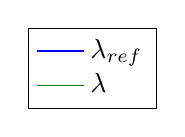
\begin{tikzpicture}

\begin{axis}[%
width=0.951\figurewidth,
height=\figureheight,
at={(0\figurewidth,0\figureheight)},
scale only axis,
every outer x axis line/.append style={black},
every x tick label/.append style={font=\color{black}},
every x tick/.append style={black},
xmin=0,
xmax=35,
xlabel={Time [s]},
every outer y axis line/.append style={black},
every y tick label/.append style={font=\color{black}},
every y tick/.append style={black},
ymin=-50,
ymax=200,
ylabel={$\lambda\text{ [deg]}$},
axis background/.style={fill=white},
axis x line*=bottom,
axis y line*=left,
xmajorgrids,
ymajorgrids,
legend style={legend cell align=left, align=left, draw=black}
]
\addplot [color=blue]
  table[row sep=crcr]{%
0	180\\
0.25	180\\
0.5	180\\
0.75	180\\
1	180\\
1.25	180\\
1.5	180\\
1.75	180\\
2	180\\
2.25	180\\
2.5	180\\
2.75	180\\
3	180\\
3.25	180\\
3.5	180\\
3.75	180\\
4	180\\
4.25	180\\
4.5	180\\
4.75	180\\
5	180\\
5.25	180\\
5.5	180\\
5.75	180\\
6	179.79\\
6.25	179.12\\
6.5	177.81\\
6.75	175.7\\
7	172.72\\
7.25	168.77\\
7.5	163.84\\
7.75	157.88\\
8	150.89\\
8.25	142.85\\
8.5	133.84\\
8.75	124.02\\
9	113.62\\
9.25	102.87\\
9.5	92.013\\
9.75	81.276\\
10	70.847\\
10.25	60.883\\
10.5	51.507\\
10.75	42.809\\
11	34.847\\
11.25	27.655\\
11.5	21.242\\
11.75	15.601\\
12	10.705\\
12.25	6.5208\\
12.5	3.0026\\
12.75	0.099717\\
13	-2.2424\\
13.25	-4.0802\\
13.5	-5.4706\\
13.75	-6.4693\\
14	-7.1301\\
14.25	-7.5036\\
14.5	-7.6374\\
14.75	-7.5749\\
15	-7.3555\\
15.25	-7.0146\\
15.5	-6.5833\\
15.75	-6.0889\\
16	-5.5545\\
16.25	-4.9998\\
16.5	-4.4412\\
16.75	-3.8919\\
17	-3.3622\\
17.25	-2.8603\\
17.5	-2.3919\\
17.75	-1.961\\
18	-1.5699\\
18.25	-1.2197\\
18.5	-0.91014\\
18.75	-0.64032\\
19	-0.40854\\
19.25	-0.2126\\
19.5	-0.049904\\
19.75	0.082356\\
20	0.18714\\
20.25	0.26743\\
20.5	0.32619\\
20.75	0.36629\\
21	0.39045\\
21.25	0.40123\\
21.5	0.40098\\
21.75	0.39184\\
22	0.37575\\
22.25	0.35441\\
22.5	0.32931\\
22.75	0.30175\\
23	0.27281\\
23.25	0.24341\\
23.5	0.2143\\
23.75	0.18605\\
24	0.15914\\
24.25	0.1339\\
24.5	0.11057\\
24.75	0.089283\\
25	0.070121\\
25.25	0.053089\\
25.5	0.038146\\
25.75	0.025209\\
26	0.014168\\
26.25	0.0048883\\
26.5	-0.002778\\
26.75	-0.0089875\\
27	-0.0139\\
27.25	-0.017674\\
27.5	-0.020462\\
27.75	-0.022413\\
28	-0.02366\\
28.25	-0.02433\\
28.5	-0.024534\\
28.75	-0.024372\\
29	-0.02393\\
29.25	-0.023278\\
29.5	-0.022475\\
29.75	-0.021568\\
30	-0.02059\\
30.25	0\\
30.5	0\\
30.75	0\\
31	0\\
31.25	0\\
31.5	0\\
31.75	0\\
32	0\\
32.25	0\\
32.5	0\\
32.75	0\\
33	0\\
33.25	0\\
33.5	0\\
33.75	0\\
34	0\\
34.25	0\\
34.5	0\\
34.75	0\\
35	0\\
};
\addlegendentry{$\lambda{}_{\text{ref}}$}

\addplot [color=black!50!green, forget plot]
  table[row sep=crcr]{%
0	180\\
0.002	180\\
0.004	180\\
0.006	180\\
0.008	180\\
0.01	180\\
0.012	180\\
0.014	180\\
0.016	180\\
0.018	180\\
0.02	180\\
0.022	180\\
0.024	180\\
0.026	180\\
0.028	180\\
0.03	180\\
0.032	180\\
0.034	180\\
0.036	180\\
0.038	180\\
0.04	180\\
0.042	180\\
0.044	180\\
0.046	180\\
0.048	180\\
0.05	180\\
0.052	180\\
0.054	180\\
0.056	180\\
0.058	180\\
0.06	180\\
0.062	180\\
0.064	180\\
0.066	180\\
0.068	180\\
0.07	180\\
0.072	180\\
0.074	180\\
0.076	180.04\\
0.078	180.04\\
0.08	180.04\\
0.082	180.04\\
0.084	180.04\\
0.086	180.04\\
0.088	180.04\\
0.09	180.04\\
0.092	180.04\\
0.094	180.04\\
0.096	180.04\\
0.098	180.04\\
0.1	180.04\\
0.102	180.04\\
0.104	180.04\\
0.106	180.04\\
0.108	180.04\\
0.11	180.04\\
0.112	180.04\\
0.114	180.04\\
0.116	180.04\\
0.118	180.09\\
0.12	180.09\\
0.122	180.09\\
0.124	180.09\\
0.126	180.09\\
0.128	180.09\\
0.13	180.09\\
0.132	180.09\\
0.134	180.09\\
0.136	180.09\\
0.138	180.09\\
0.14	180.09\\
0.142	180.09\\
0.144	180.09\\
0.146	180.09\\
0.148	180.13\\
0.15	180.13\\
0.152	180.13\\
0.154	180.13\\
0.156	180.13\\
0.158	180.13\\
0.16	180.13\\
0.162	180.13\\
0.164	180.13\\
0.166	180.13\\
0.168	180.13\\
0.17	180.13\\
0.172	180.18\\
0.174	180.18\\
0.176	180.18\\
0.178	180.18\\
0.18	180.18\\
0.182	180.18\\
0.184	180.18\\
0.186	180.18\\
0.188	180.22\\
0.19	180.22\\
0.192	180.22\\
0.194	180.22\\
0.196	180.22\\
0.198	180.22\\
0.2	180.22\\
0.202	180.22\\
0.204	180.22\\
0.206	180.22\\
0.208	180.22\\
0.21	180.26\\
0.212	180.26\\
0.214	180.26\\
0.216	180.26\\
0.218	180.26\\
0.22	180.26\\
0.222	180.26\\
0.224	180.26\\
0.226	180.26\\
0.228	180.26\\
0.23	180.26\\
0.232	180.31\\
0.234	180.31\\
0.236	180.31\\
0.238	180.31\\
0.24	180.35\\
0.242	180.35\\
0.244	180.35\\
0.246	180.35\\
0.248	180.35\\
0.25	180.35\\
0.252	180.35\\
0.254	180.35\\
0.256	180.35\\
0.258	180.35\\
0.26	180.35\\
0.262	180.4\\
0.264	180.4\\
0.266	180.4\\
0.268	180.4\\
0.27	180.4\\
0.272	180.4\\
0.274	180.44\\
0.276	180.44\\
0.278	180.44\\
0.28	180.44\\
0.282	180.44\\
0.284	180.44\\
0.286	180.44\\
0.288	180.48\\
0.29	180.48\\
0.292	180.48\\
0.294	180.48\\
0.296	180.48\\
0.298	180.48\\
0.3	180.48\\
0.302	180.53\\
0.304	180.53\\
0.306	180.53\\
0.308	180.53\\
0.31	180.53\\
0.312	180.53\\
0.314	180.53\\
0.316	180.57\\
0.318	180.57\\
0.32	180.57\\
0.322	180.57\\
0.324	180.57\\
0.326	180.57\\
0.328	180.57\\
0.33	180.62\\
0.332	180.62\\
0.334	180.62\\
0.336	180.62\\
0.338	180.62\\
0.34	180.62\\
0.342	180.62\\
0.344	180.66\\
0.346	180.7\\
0.348	180.7\\
0.35	180.66\\
0.352	180.66\\
0.354	180.66\\
0.356	180.66\\
0.358	180.7\\
0.36	180.7\\
0.362	180.7\\
0.364	180.7\\
0.366	180.66\\
0.368	180.7\\
0.37	180.75\\
0.372	180.79\\
0.374	180.79\\
0.376	180.79\\
0.378	180.75\\
0.38	180.75\\
0.382	180.75\\
0.384	180.79\\
0.386	180.83\\
0.388	180.83\\
0.39	180.79\\
0.392	180.79\\
0.394	180.79\\
0.396	180.79\\
0.398	180.83\\
0.4	180.88\\
0.402	180.88\\
0.404	180.83\\
0.406	180.83\\
0.408	180.83\\
0.41	180.88\\
0.412	180.92\\
0.414	180.92\\
0.416	180.92\\
0.418	180.88\\
0.42	180.88\\
0.422	180.88\\
0.424	180.92\\
0.426	180.97\\
0.428	181.01\\
0.43	180.97\\
0.432	180.92\\
0.434	180.92\\
0.436	180.97\\
0.438	181.01\\
0.44	181.05\\
0.442	181.05\\
0.444	181.01\\
0.446	180.97\\
0.448	180.97\\
0.45	181.01\\
0.452	181.05\\
0.454	181.1\\
0.456	181.05\\
0.458	181.01\\
0.46	181.01\\
0.462	181.01\\
0.464	181.1\\
0.466	181.14\\
0.468	181.14\\
0.47	181.1\\
0.472	181.05\\
0.474	181.05\\
0.476	181.1\\
0.478	181.14\\
0.48	181.19\\
0.482	181.19\\
0.484	181.14\\
0.486	181.1\\
0.488	181.1\\
0.49	181.14\\
0.492	181.19\\
0.494	181.23\\
0.496	181.23\\
0.498	181.19\\
0.5	181.14\\
0.502	181.19\\
0.504	181.19\\
0.506	181.27\\
0.508	181.27\\
0.51	181.27\\
0.512	181.23\\
0.514	181.23\\
0.516	181.23\\
0.518	181.27\\
0.52	181.27\\
0.522	181.32\\
0.524	181.32\\
0.526	181.27\\
0.528	181.27\\
0.53	181.27\\
0.532	181.32\\
0.534	181.32\\
0.536	181.36\\
0.538	181.36\\
0.54	181.32\\
0.542	181.32\\
0.544	181.32\\
0.546	181.36\\
0.548	181.36\\
0.55	181.36\\
0.552	181.36\\
0.554	181.36\\
0.556	181.36\\
0.558	181.41\\
0.56	181.41\\
0.562	181.41\\
0.564	181.41\\
0.566	181.41\\
0.568	181.41\\
0.57	181.45\\
0.572	181.45\\
0.574	181.45\\
0.576	181.45\\
0.578	181.45\\
0.58	181.45\\
0.582	181.45\\
0.584	181.49\\
0.586	181.49\\
0.588	181.49\\
0.59	181.49\\
0.592	181.49\\
0.594	181.49\\
0.596	181.49\\
0.598	181.54\\
0.6	181.54\\
0.602	181.54\\
0.604	181.54\\
0.606	181.54\\
0.608	181.54\\
0.61	181.54\\
0.612	181.58\\
0.614	181.58\\
0.616	181.58\\
0.618	181.58\\
0.62	181.58\\
0.622	181.58\\
0.624	181.58\\
0.626	181.58\\
0.628	181.63\\
0.63	181.63\\
0.632	181.63\\
0.634	181.63\\
0.636	181.63\\
0.638	181.63\\
0.64	181.63\\
0.642	181.67\\
0.644	181.67\\
0.646	181.67\\
0.648	181.67\\
0.65	181.67\\
0.652	181.67\\
0.654	181.67\\
0.656	181.67\\
0.658	181.71\\
0.66	181.71\\
0.662	181.71\\
0.664	181.71\\
0.666	181.71\\
0.668	181.71\\
0.67	181.71\\
0.672	181.71\\
0.674	181.76\\
0.676	181.76\\
0.678	181.76\\
0.68	181.76\\
0.682	181.76\\
0.684	181.76\\
0.686	181.76\\
0.688	181.76\\
0.69	181.8\\
0.692	181.8\\
0.694	181.8\\
0.696	181.8\\
0.698	181.8\\
0.7	181.8\\
0.702	181.8\\
0.704	181.8\\
0.706	181.85\\
0.708	181.85\\
0.71	181.85\\
0.712	181.85\\
0.714	181.85\\
0.716	181.85\\
0.718	181.85\\
0.72	181.85\\
0.722	181.85\\
0.724	181.85\\
0.726	181.89\\
0.728	181.89\\
0.73	181.89\\
0.732	181.89\\
0.734	181.89\\
0.736	181.89\\
0.738	181.89\\
0.74	181.89\\
0.742	181.89\\
0.744	181.89\\
0.746	181.89\\
0.748	181.93\\
0.75	181.93\\
0.752	181.93\\
0.754	181.93\\
0.756	181.93\\
0.758	181.93\\
0.76	181.93\\
0.762	181.98\\
0.764	181.98\\
0.766	181.98\\
0.768	181.98\\
0.77	181.98\\
0.772	181.98\\
0.774	181.98\\
0.776	181.98\\
0.778	181.98\\
0.78	181.98\\
0.782	181.98\\
0.784	181.98\\
0.786	182.02\\
0.788	182.02\\
0.79	182.02\\
0.792	182.02\\
0.794	182.02\\
0.796	182.02\\
0.798	182.02\\
0.8	182.02\\
0.802	182.02\\
0.804	182.02\\
0.806	182.07\\
0.808	182.07\\
0.81	182.07\\
0.812	182.07\\
0.814	182.07\\
0.816	182.07\\
0.818	182.07\\
0.82	182.07\\
0.822	182.07\\
0.824	182.07\\
0.826	182.07\\
0.828	182.11\\
0.83	182.11\\
0.832	182.11\\
0.834	182.11\\
0.836	182.11\\
0.838	182.11\\
0.84	182.11\\
0.842	182.11\\
0.844	182.11\\
0.846	182.11\\
0.848	182.11\\
0.85	182.15\\
0.852	182.15\\
0.854	182.15\\
0.856	182.15\\
0.858	182.15\\
0.86	182.15\\
0.862	182.15\\
0.864	182.15\\
0.866	182.15\\
0.868	182.15\\
0.87	182.15\\
0.872	182.15\\
0.874	182.2\\
0.876	182.2\\
0.878	182.2\\
0.88	182.2\\
0.882	182.2\\
0.884	182.2\\
0.886	182.2\\
0.888	182.2\\
0.89	182.2\\
0.892	182.2\\
0.894	182.2\\
0.896	182.2\\
0.898	182.2\\
0.9	182.2\\
0.902	182.24\\
0.904	182.24\\
0.906	182.24\\
0.908	182.24\\
0.91	182.24\\
0.912	182.24\\
0.914	182.24\\
0.916	182.24\\
0.918	182.24\\
0.92	182.24\\
0.922	182.24\\
0.924	182.24\\
0.926	182.29\\
0.928	182.29\\
0.93	182.29\\
0.932	182.29\\
0.934	182.29\\
0.936	182.29\\
0.938	182.29\\
0.94	182.29\\
0.942	182.29\\
0.944	182.29\\
0.946	182.29\\
0.948	182.29\\
0.95	182.29\\
0.952	182.33\\
0.954	182.33\\
0.956	182.33\\
0.958	182.33\\
0.96	182.33\\
0.962	182.33\\
0.964	182.33\\
0.966	182.33\\
0.968	182.33\\
0.97	182.33\\
0.972	182.33\\
0.974	182.33\\
0.976	182.33\\
0.978	182.33\\
0.98	182.37\\
0.982	182.37\\
0.984	182.37\\
0.986	182.37\\
0.988	182.37\\
0.99	182.37\\
0.992	182.37\\
0.994	182.37\\
0.996	182.37\\
0.998	182.37\\
1	182.37\\
1.002	182.37\\
1.004	182.37\\
1.006	182.37\\
1.008	182.37\\
1.01	182.37\\
1.012	182.37\\
1.014	182.37\\
1.016	182.37\\
1.018	182.42\\
1.02	182.42\\
1.022	182.42\\
1.024	182.42\\
1.026	182.42\\
1.028	182.42\\
1.03	182.42\\
1.032	182.42\\
1.034	182.42\\
1.036	182.42\\
1.038	182.42\\
1.04	182.42\\
1.042	182.42\\
1.044	182.42\\
1.046	182.46\\
1.048	182.46\\
1.05	182.46\\
1.052	182.46\\
1.054	182.46\\
1.056	182.46\\
1.058	182.46\\
1.06	182.46\\
1.062	182.46\\
1.064	182.46\\
1.066	182.46\\
1.068	182.46\\
1.07	182.46\\
1.072	182.46\\
1.074	182.46\\
1.076	182.5\\
1.078	182.5\\
1.08	182.5\\
1.082	182.5\\
1.084	182.46\\
1.086	182.46\\
1.088	182.46\\
1.09	182.5\\
1.092	182.5\\
1.094	182.5\\
1.096	182.5\\
1.098	182.5\\
1.1	182.5\\
1.102	182.5\\
1.104	182.5\\
1.106	182.5\\
1.108	182.5\\
1.11	182.5\\
1.112	182.5\\
1.114	182.5\\
1.116	182.5\\
1.118	182.5\\
1.12	182.5\\
1.122	182.55\\
1.124	182.55\\
1.126	182.55\\
1.128	182.55\\
1.13	182.55\\
1.132	182.55\\
1.134	182.55\\
1.136	182.55\\
1.138	182.55\\
1.14	182.55\\
1.142	182.55\\
1.144	182.55\\
1.146	182.55\\
1.148	182.55\\
1.15	182.55\\
1.152	182.55\\
1.154	182.59\\
1.156	182.59\\
1.158	182.59\\
1.16	182.59\\
1.162	182.59\\
1.164	182.59\\
1.166	182.59\\
1.168	182.59\\
1.17	182.59\\
1.172	182.59\\
1.174	182.59\\
1.176	182.59\\
1.178	182.59\\
1.18	182.59\\
1.182	182.59\\
1.184	182.59\\
1.186	182.59\\
1.188	182.59\\
1.19	182.59\\
1.192	182.59\\
1.194	182.59\\
1.196	182.59\\
1.198	182.59\\
1.2	182.64\\
1.202	182.64\\
1.204	182.64\\
1.206	182.64\\
1.208	182.64\\
1.21	182.64\\
1.212	182.64\\
1.214	182.64\\
1.216	182.64\\
1.218	182.64\\
1.22	182.64\\
1.222	182.64\\
1.224	182.64\\
1.226	182.64\\
1.228	182.64\\
1.23	182.68\\
1.232	182.68\\
1.234	182.68\\
1.236	182.68\\
1.238	182.64\\
1.24	182.64\\
1.242	182.64\\
1.244	182.64\\
1.246	182.64\\
1.248	182.64\\
1.25	182.68\\
1.252	182.68\\
1.254	182.68\\
1.256	182.68\\
1.258	182.68\\
1.26	182.68\\
1.262	182.68\\
1.264	182.68\\
1.266	182.68\\
1.268	182.68\\
1.27	182.68\\
1.272	182.68\\
1.274	182.68\\
1.276	182.68\\
1.278	182.68\\
1.28	182.68\\
1.282	182.72\\
1.284	182.72\\
1.286	182.72\\
1.288	182.72\\
1.29	182.72\\
1.292	182.72\\
1.294	182.72\\
1.296	182.72\\
1.298	182.72\\
1.3	182.72\\
1.302	182.72\\
1.304	182.72\\
1.306	182.72\\
1.308	182.72\\
1.31	182.72\\
1.312	182.72\\
1.314	182.72\\
1.316	182.72\\
1.318	182.72\\
1.32	182.72\\
1.322	182.72\\
1.324	182.72\\
1.326	182.72\\
1.328	182.72\\
1.33	182.72\\
1.332	182.72\\
1.334	182.72\\
1.336	182.77\\
1.338	182.77\\
1.34	182.77\\
1.342	182.77\\
1.344	182.77\\
1.346	182.77\\
1.348	182.77\\
1.35	182.77\\
1.352	182.77\\
1.354	182.77\\
1.356	182.77\\
1.358	182.77\\
1.36	182.77\\
1.362	182.77\\
1.364	182.77\\
1.366	182.77\\
1.368	182.77\\
1.37	182.77\\
1.372	182.77\\
1.374	182.77\\
1.376	182.77\\
1.378	182.77\\
1.38	182.77\\
1.382	182.77\\
1.384	182.77\\
1.386	182.81\\
1.388	182.81\\
1.39	182.81\\
1.392	182.81\\
1.394	182.81\\
1.396	182.81\\
1.398	182.81\\
1.4	182.81\\
1.402	182.81\\
1.404	182.81\\
1.406	182.81\\
1.408	182.81\\
1.41	182.81\\
1.412	182.81\\
1.414	182.81\\
1.416	182.81\\
1.418	182.81\\
1.42	182.86\\
1.422	182.86\\
1.424	182.86\\
1.426	182.86\\
1.428	182.81\\
1.43	182.81\\
1.432	182.81\\
1.434	182.81\\
1.436	182.81\\
1.438	182.86\\
1.44	182.86\\
1.442	182.86\\
1.444	182.86\\
1.446	182.86\\
1.448	182.86\\
1.45	182.86\\
1.452	182.86\\
1.454	182.86\\
1.456	182.86\\
1.458	182.86\\
1.46	182.86\\
1.462	182.86\\
1.464	182.86\\
1.466	182.86\\
1.468	182.9\\
1.47	182.9\\
1.472	182.9\\
1.474	182.9\\
1.476	182.9\\
1.478	182.9\\
1.48	182.86\\
1.482	182.86\\
1.484	182.86\\
1.486	182.86\\
1.488	182.9\\
1.49	182.9\\
1.492	182.9\\
1.494	182.9\\
1.496	182.9\\
1.498	182.9\\
1.5	182.9\\
1.502	182.9\\
1.504	182.9\\
1.506	182.9\\
1.508	182.9\\
1.51	182.9\\
1.512	182.9\\
1.514	182.9\\
1.516	182.9\\
1.518	182.9\\
1.52	182.94\\
1.522	182.94\\
1.524	182.94\\
1.526	182.94\\
1.528	182.9\\
1.53	182.9\\
1.532	182.9\\
1.534	182.9\\
1.536	182.9\\
1.538	182.9\\
1.54	182.94\\
1.542	182.94\\
1.544	182.94\\
1.546	182.94\\
1.548	182.94\\
1.55	182.94\\
1.552	182.94\\
1.554	182.94\\
1.556	182.94\\
1.558	182.94\\
1.56	182.94\\
1.562	182.94\\
1.564	182.94\\
1.566	182.94\\
1.568	182.94\\
1.57	182.99\\
1.572	182.99\\
1.574	182.99\\
1.576	182.99\\
1.578	182.94\\
1.58	182.94\\
1.582	182.94\\
1.584	182.94\\
1.586	182.94\\
1.588	182.99\\
1.59	182.99\\
1.592	182.99\\
1.594	182.99\\
1.596	182.99\\
1.598	182.99\\
1.6	182.99\\
1.602	182.99\\
1.604	182.99\\
1.606	182.99\\
1.608	182.99\\
1.61	182.99\\
1.612	182.99\\
1.614	182.99\\
1.616	182.99\\
1.618	182.99\\
1.62	182.99\\
1.622	182.99\\
1.624	182.99\\
1.626	182.99\\
1.628	182.99\\
1.63	182.99\\
1.632	182.99\\
1.634	182.99\\
1.636	183.03\\
1.638	183.03\\
1.64	183.03\\
1.642	183.03\\
1.644	183.03\\
1.646	183.03\\
1.648	183.03\\
1.65	183.03\\
1.652	183.03\\
1.654	183.03\\
1.656	183.03\\
1.658	183.03\\
1.66	183.03\\
1.662	183.03\\
1.664	183.03\\
1.666	183.03\\
1.668	183.03\\
1.67	183.03\\
1.672	183.03\\
1.674	183.03\\
1.676	183.03\\
1.678	183.03\\
1.68	183.03\\
1.682	183.03\\
1.684	183.08\\
1.686	183.08\\
1.688	183.08\\
1.69	183.08\\
1.692	183.08\\
1.694	183.08\\
1.696	183.08\\
1.698	183.08\\
1.7	183.08\\
1.702	183.08\\
1.704	183.08\\
1.706	183.08\\
1.708	183.08\\
1.71	183.08\\
1.712	183.08\\
1.714	183.08\\
1.716	183.08\\
1.718	183.08\\
1.72	183.08\\
1.722	183.08\\
1.724	183.08\\
1.726	183.08\\
1.728	183.08\\
1.73	183.08\\
1.732	183.08\\
1.734	183.08\\
1.736	183.08\\
1.738	183.08\\
1.74	183.08\\
1.742	183.08\\
1.744	183.08\\
1.746	183.08\\
1.748	183.12\\
1.75	183.12\\
1.752	183.12\\
1.754	183.12\\
1.756	183.12\\
1.758	183.12\\
1.76	183.12\\
1.762	183.12\\
1.764	183.12\\
1.766	183.12\\
1.768	183.12\\
1.77	183.12\\
1.772	183.12\\
1.774	183.12\\
1.776	183.12\\
1.778	183.12\\
1.78	183.12\\
1.782	183.12\\
1.784	183.12\\
1.786	183.12\\
1.788	183.12\\
1.79	183.12\\
1.792	183.12\\
1.794	183.12\\
1.796	183.12\\
1.798	183.12\\
1.8	183.12\\
1.802	183.16\\
1.804	183.16\\
1.806	183.16\\
1.808	183.16\\
1.81	183.16\\
1.812	183.16\\
1.814	183.16\\
1.816	183.16\\
1.818	183.16\\
1.82	183.16\\
1.822	183.16\\
1.824	183.16\\
1.826	183.16\\
1.828	183.16\\
1.83	183.16\\
1.832	183.16\\
1.834	183.16\\
1.836	183.16\\
1.838	183.16\\
1.84	183.16\\
1.842	183.16\\
1.844	183.16\\
1.846	183.16\\
1.848	183.16\\
1.85	183.16\\
1.852	183.16\\
1.854	183.21\\
1.856	183.21\\
1.858	183.21\\
1.86	183.21\\
1.862	183.21\\
1.864	183.21\\
1.866	183.21\\
1.868	183.21\\
1.87	183.21\\
1.872	183.21\\
1.874	183.21\\
1.876	183.21\\
1.878	183.21\\
1.88	183.21\\
1.882	183.21\\
1.884	183.21\\
1.886	183.21\\
1.888	183.21\\
1.89	183.21\\
1.892	183.21\\
1.894	183.21\\
1.896	183.21\\
1.898	183.21\\
1.9	183.25\\
1.902	183.25\\
1.904	183.21\\
1.906	183.21\\
1.908	183.25\\
1.91	183.25\\
1.912	183.25\\
1.914	183.25\\
1.916	183.21\\
1.918	183.25\\
1.92	183.25\\
1.922	183.25\\
1.924	183.25\\
1.926	183.25\\
1.928	183.25\\
1.93	183.25\\
1.932	183.25\\
1.934	183.25\\
1.936	183.25\\
1.938	183.25\\
1.94	183.25\\
1.942	183.25\\
1.944	183.25\\
1.946	183.25\\
1.948	183.25\\
1.95	183.25\\
1.952	183.3\\
1.954	183.25\\
1.956	183.25\\
1.958	183.25\\
1.96	183.25\\
1.962	183.3\\
1.964	183.3\\
1.966	183.3\\
1.968	183.3\\
1.97	183.3\\
1.972	183.3\\
1.974	183.3\\
1.976	183.3\\
1.978	183.3\\
1.98	183.3\\
1.982	183.3\\
1.984	183.3\\
1.986	183.3\\
1.988	183.3\\
1.99	183.3\\
1.992	183.3\\
1.994	183.3\\
1.996	183.3\\
1.998	183.3\\
2	183.3\\
2.002	183.3\\
2.004	183.3\\
2.006	183.3\\
2.008	183.3\\
2.01	183.3\\
2.012	183.3\\
2.014	183.34\\
2.016	183.34\\
2.018	183.3\\
2.02	183.3\\
2.022	183.3\\
2.024	183.34\\
2.026	183.34\\
2.028	183.34\\
2.03	183.34\\
2.032	183.34\\
2.034	183.34\\
2.036	183.34\\
2.038	183.34\\
2.04	183.34\\
2.042	183.34\\
2.044	183.34\\
2.046	183.34\\
2.048	183.34\\
2.05	183.34\\
2.052	183.34\\
2.054	183.34\\
2.056	183.34\\
2.058	183.34\\
2.06	183.34\\
2.062	183.34\\
2.064	183.34\\
2.066	183.34\\
2.068	183.38\\
2.07	183.38\\
2.072	183.38\\
2.074	183.38\\
2.076	183.38\\
2.078	183.38\\
2.08	183.38\\
2.082	183.38\\
2.084	183.38\\
2.086	183.38\\
2.088	183.38\\
2.09	183.38\\
2.092	183.38\\
2.094	183.38\\
2.096	183.38\\
2.098	183.38\\
2.1	183.38\\
2.102	183.38\\
2.104	183.38\\
2.106	183.38\\
2.108	183.38\\
2.11	183.38\\
2.112	183.38\\
2.114	183.38\\
2.116	183.38\\
2.118	183.38\\
2.12	183.38\\
2.122	183.38\\
2.124	183.43\\
2.126	183.43\\
2.128	183.38\\
2.13	183.38\\
2.132	183.43\\
2.134	183.43\\
2.136	183.43\\
2.138	183.43\\
2.14	183.43\\
2.142	183.43\\
2.144	183.43\\
2.146	183.43\\
2.148	183.43\\
2.15	183.43\\
2.152	183.43\\
2.154	183.43\\
2.156	183.43\\
2.158	183.43\\
2.16	183.43\\
2.162	183.43\\
2.164	183.43\\
2.166	183.43\\
2.168	183.43\\
2.17	183.43\\
2.172	183.43\\
2.174	183.43\\
2.176	183.43\\
2.178	183.43\\
2.18	183.43\\
2.182	183.43\\
2.184	183.43\\
2.186	183.47\\
2.188	183.47\\
2.19	183.47\\
2.192	183.47\\
2.194	183.47\\
2.196	183.47\\
2.198	183.47\\
2.2	183.47\\
2.202	183.47\\
2.204	183.47\\
2.206	183.47\\
2.208	183.47\\
2.21	183.47\\
2.212	183.47\\
2.214	183.47\\
2.216	183.47\\
2.218	183.47\\
2.22	183.47\\
2.222	183.47\\
2.224	183.47\\
2.226	183.47\\
2.228	183.47\\
2.23	183.47\\
2.232	183.47\\
2.234	183.47\\
2.236	183.47\\
2.238	183.47\\
2.24	183.47\\
2.242	183.52\\
2.244	183.52\\
2.246	183.52\\
2.248	183.52\\
2.25	183.52\\
2.252	183.52\\
2.254	183.52\\
2.256	183.52\\
2.258	183.52\\
2.26	183.52\\
2.262	183.52\\
2.264	183.52\\
2.266	183.52\\
2.268	183.52\\
2.27	183.52\\
2.272	183.52\\
2.274	183.52\\
2.276	183.52\\
2.278	183.52\\
2.28	183.52\\
2.282	183.52\\
2.284	183.52\\
2.286	183.52\\
2.288	183.52\\
2.29	183.52\\
2.292	183.52\\
2.294	183.56\\
2.296	183.56\\
2.298	183.56\\
2.3	183.56\\
2.302	183.56\\
2.304	183.56\\
2.306	183.56\\
2.308	183.56\\
2.31	183.56\\
2.312	183.56\\
2.314	183.56\\
2.316	183.56\\
2.318	183.56\\
2.32	183.56\\
2.322	183.56\\
2.324	183.56\\
2.326	183.56\\
2.328	183.56\\
2.33	183.56\\
2.332	183.56\\
2.334	183.56\\
2.336	183.56\\
2.338	183.56\\
2.34	183.56\\
2.342	183.56\\
2.344	183.56\\
2.346	183.6\\
2.348	183.6\\
2.35	183.6\\
2.352	183.6\\
2.354	183.6\\
2.356	183.56\\
2.358	183.6\\
2.36	183.6\\
2.362	183.6\\
2.364	183.6\\
2.366	183.6\\
2.368	183.6\\
2.37	183.6\\
2.372	183.6\\
2.374	183.6\\
2.376	183.6\\
2.378	183.6\\
2.38	183.6\\
2.382	183.6\\
2.384	183.6\\
2.386	183.6\\
2.388	183.6\\
2.39	183.6\\
2.392	183.6\\
2.394	183.6\\
2.396	183.6\\
2.398	183.6\\
2.4	183.6\\
2.402	183.6\\
2.404	183.6\\
2.406	183.6\\
2.408	183.6\\
2.41	183.6\\
2.412	183.65\\
2.414	183.65\\
2.416	183.65\\
2.418	183.65\\
2.42	183.65\\
2.422	183.65\\
2.424	183.65\\
2.426	183.65\\
2.428	183.65\\
2.43	183.65\\
2.432	183.65\\
2.434	183.65\\
2.436	183.65\\
2.438	183.65\\
2.44	183.65\\
2.442	183.65\\
2.444	183.65\\
2.446	183.65\\
2.448	183.65\\
2.45	183.65\\
2.452	183.65\\
2.454	183.65\\
2.456	183.65\\
2.458	183.65\\
2.46	183.65\\
2.462	183.65\\
2.464	183.65\\
2.466	183.65\\
2.468	183.69\\
2.47	183.69\\
2.472	183.69\\
2.474	183.69\\
2.476	183.69\\
2.478	183.69\\
2.48	183.69\\
2.482	183.69\\
2.484	183.69\\
2.486	183.69\\
2.488	183.69\\
2.49	183.69\\
2.492	183.69\\
2.494	183.69\\
2.496	183.69\\
2.498	183.69\\
2.5	183.69\\
2.502	183.69\\
2.504	183.69\\
2.506	183.69\\
2.508	183.69\\
2.51	183.69\\
2.512	183.69\\
2.514	183.69\\
2.516	183.69\\
2.518	183.69\\
2.52	183.69\\
2.522	183.69\\
2.524	183.69\\
2.526	183.74\\
2.528	183.74\\
2.53	183.74\\
2.532	183.74\\
2.534	183.74\\
2.536	183.74\\
2.538	183.74\\
2.54	183.74\\
2.542	183.74\\
2.544	183.74\\
2.546	183.74\\
2.548	183.74\\
2.55	183.74\\
2.552	183.74\\
2.554	183.74\\
2.556	183.74\\
2.558	183.74\\
2.56	183.74\\
2.562	183.74\\
2.564	183.74\\
2.566	183.74\\
2.568	183.74\\
2.57	183.74\\
2.572	183.74\\
2.574	183.74\\
2.576	183.74\\
2.578	183.74\\
2.58	183.74\\
2.582	183.74\\
2.584	183.74\\
2.586	183.74\\
2.588	183.74\\
2.59	183.78\\
2.592	183.78\\
2.594	183.78\\
2.596	183.78\\
2.598	183.78\\
2.6	183.78\\
2.602	183.78\\
2.604	183.78\\
2.606	183.78\\
2.608	183.78\\
2.61	183.78\\
2.612	183.78\\
2.614	183.78\\
2.616	183.78\\
2.618	183.78\\
2.62	183.78\\
2.622	183.78\\
2.624	183.78\\
2.626	183.78\\
2.628	183.78\\
2.63	183.78\\
2.632	183.78\\
2.634	183.78\\
2.636	183.78\\
2.638	183.78\\
2.64	183.78\\
2.642	183.78\\
2.644	183.78\\
2.646	183.78\\
2.648	183.78\\
2.65	183.78\\
2.652	183.78\\
2.654	183.82\\
2.656	183.82\\
2.658	183.82\\
2.66	183.82\\
2.662	183.82\\
2.664	183.82\\
2.666	183.82\\
2.668	183.82\\
2.67	183.82\\
2.672	183.82\\
2.674	183.82\\
2.676	183.82\\
2.678	183.82\\
2.68	183.82\\
2.682	183.82\\
2.684	183.82\\
2.686	183.82\\
2.688	183.82\\
2.69	183.82\\
2.692	183.82\\
2.694	183.82\\
2.696	183.82\\
2.698	183.82\\
2.7	183.82\\
2.702	183.82\\
2.704	183.82\\
2.706	183.82\\
2.708	183.82\\
2.71	183.82\\
2.712	183.82\\
2.714	183.82\\
2.716	183.82\\
2.718	183.82\\
2.72	183.82\\
2.722	183.82\\
2.724	183.82\\
2.726	183.82\\
2.728	183.82\\
2.73	183.82\\
2.732	183.87\\
2.734	183.87\\
2.736	183.87\\
2.738	183.87\\
2.74	183.87\\
2.742	183.87\\
2.744	183.87\\
2.746	183.87\\
2.748	183.87\\
2.75	183.87\\
2.752	183.87\\
2.754	183.87\\
2.756	183.87\\
2.758	183.87\\
2.76	183.87\\
2.762	183.87\\
2.764	183.87\\
2.766	183.87\\
2.768	183.87\\
2.77	183.87\\
2.772	183.87\\
2.774	183.87\\
2.776	183.87\\
2.778	183.87\\
2.78	183.87\\
2.782	183.87\\
2.784	183.87\\
2.786	183.87\\
2.788	183.87\\
2.79	183.87\\
2.792	183.87\\
2.794	183.87\\
2.796	183.87\\
2.798	183.87\\
2.8	183.87\\
2.802	183.87\\
2.804	183.87\\
2.806	183.87\\
2.808	183.87\\
2.81	183.91\\
2.812	183.91\\
2.814	183.91\\
2.816	183.91\\
2.818	183.91\\
2.82	183.91\\
2.822	183.91\\
2.824	183.91\\
2.826	183.91\\
2.828	183.91\\
2.83	183.91\\
2.832	183.91\\
2.834	183.91\\
2.836	183.91\\
2.838	183.91\\
2.84	183.91\\
2.842	183.91\\
2.844	183.91\\
2.846	183.91\\
2.848	183.91\\
2.85	183.91\\
2.852	183.91\\
2.854	183.91\\
2.856	183.91\\
2.858	183.91\\
2.86	183.91\\
2.862	183.91\\
2.864	183.91\\
2.866	183.91\\
2.868	183.91\\
2.87	183.91\\
2.872	183.91\\
2.874	183.91\\
2.876	183.91\\
2.878	183.91\\
2.88	183.91\\
2.882	183.91\\
2.884	183.91\\
2.886	183.91\\
2.888	183.96\\
2.89	183.96\\
2.892	183.96\\
2.894	183.96\\
2.896	183.91\\
2.898	183.91\\
2.9	183.91\\
2.902	183.96\\
2.904	183.96\\
2.906	183.96\\
2.908	183.96\\
2.91	183.96\\
2.912	183.96\\
2.914	183.96\\
2.916	183.96\\
2.918	183.96\\
2.92	183.96\\
2.922	183.96\\
2.924	183.96\\
2.926	183.96\\
2.928	183.96\\
2.93	183.96\\
2.932	183.96\\
2.934	183.96\\
2.936	183.96\\
2.938	183.96\\
2.94	183.96\\
2.942	183.96\\
2.944	183.96\\
2.946	183.96\\
2.948	183.96\\
2.95	183.96\\
2.952	183.96\\
2.954	183.96\\
2.956	183.96\\
2.958	183.96\\
2.96	183.96\\
2.962	183.96\\
2.964	183.96\\
2.966	183.96\\
2.968	183.96\\
2.97	183.96\\
2.972	183.96\\
2.974	183.96\\
2.976	183.96\\
2.978	183.96\\
2.98	183.96\\
2.982	183.96\\
2.984	183.96\\
2.986	183.96\\
2.988	183.96\\
2.99	183.96\\
2.992	183.96\\
2.994	183.96\\
2.996	183.96\\
2.998	183.96\\
3	183.96\\
3.002	183.96\\
3.004	183.96\\
3.006	183.96\\
3.008	183.96\\
3.01	183.96\\
3.012	184\\
3.014	184\\
3.016	184\\
3.018	184\\
3.02	184\\
3.022	184\\
3.024	184\\
3.026	184\\
3.028	184\\
3.03	184\\
3.032	184\\
3.034	184\\
3.036	184\\
3.038	184\\
3.04	184\\
3.042	184\\
3.044	184\\
3.046	184\\
3.048	184\\
3.05	184\\
3.052	184\\
3.054	184\\
3.056	184\\
3.058	184\\
3.06	184\\
3.062	184\\
3.064	184\\
3.066	184\\
3.068	184\\
3.07	184\\
3.072	184\\
3.074	184\\
3.076	184\\
3.078	184\\
3.08	184\\
3.082	184\\
3.084	184\\
3.086	184\\
3.088	184\\
3.09	184\\
3.092	184\\
3.094	184\\
3.096	184\\
3.098	184\\
3.1	184\\
3.102	184\\
3.104	184\\
3.106	184\\
3.108	184\\
3.11	184\\
3.112	184\\
3.114	184\\
3.116	184\\
3.118	184\\
3.12	184\\
3.122	184\\
3.124	184\\
3.126	184\\
3.128	184\\
3.13	184\\
3.132	184\\
3.134	184\\
3.136	184\\
3.138	184\\
3.14	184\\
3.142	184\\
3.144	184\\
3.146	184\\
3.148	184\\
3.15	184\\
3.152	184.04\\
3.154	184.04\\
3.156	184.04\\
3.158	184.04\\
3.16	184\\
3.162	184\\
3.164	184\\
3.166	184.04\\
3.168	184.04\\
3.17	184.04\\
3.172	184.04\\
3.174	184.04\\
3.176	184.04\\
3.178	184\\
3.18	184.04\\
3.182	184.04\\
3.184	184.04\\
3.186	184.04\\
3.188	184.04\\
3.19	184.04\\
3.192	184.04\\
3.194	184.04\\
3.196	184.04\\
3.198	184.04\\
3.2	184.04\\
3.202	184.04\\
3.204	184.04\\
3.206	184.04\\
3.208	184.04\\
3.21	184.04\\
3.212	184.04\\
3.214	184.04\\
3.216	184.04\\
3.218	184.04\\
3.22	184.04\\
3.222	184.04\\
3.224	184.04\\
3.226	184.04\\
3.228	184.04\\
3.23	184.04\\
3.232	184.04\\
3.234	184.04\\
3.236	184.04\\
3.238	184.04\\
3.24	184.04\\
3.242	184.04\\
3.244	184.04\\
3.246	184.04\\
3.248	184.04\\
3.25	184.04\\
3.252	184.04\\
3.254	184.04\\
3.256	184.04\\
3.258	184.04\\
3.26	184.04\\
3.262	184.04\\
3.264	184.04\\
3.266	184.04\\
3.268	184.04\\
3.27	184.04\\
3.272	184.04\\
3.274	184.04\\
3.276	184.04\\
3.278	184.04\\
3.28	184.04\\
3.282	184.04\\
3.284	184.04\\
3.286	184.04\\
3.288	184.04\\
3.29	184.04\\
3.292	184.04\\
3.294	184.04\\
3.296	184.04\\
3.298	184.04\\
3.3	184.04\\
3.302	184.04\\
3.304	184.04\\
3.306	184.04\\
3.308	184.04\\
3.31	184.04\\
3.312	184.04\\
3.314	184.04\\
3.316	184.04\\
3.318	184.04\\
3.32	184.04\\
3.322	184.04\\
3.324	184.04\\
3.326	184.04\\
3.328	184.04\\
3.33	184.04\\
3.332	184.04\\
3.334	184.04\\
3.336	184.04\\
3.338	184.04\\
3.34	184.04\\
3.342	184.04\\
3.344	184.04\\
3.346	184.04\\
3.348	184.04\\
3.35	184.04\\
3.352	184.04\\
3.354	184.04\\
3.356	184.04\\
3.358	184.04\\
3.36	184.04\\
3.362	184.04\\
3.364	184.04\\
3.366	184.04\\
3.368	184.04\\
3.37	184.04\\
3.372	184.04\\
3.374	184.04\\
3.376	184.04\\
3.378	184.04\\
3.38	184.04\\
3.382	184.04\\
3.384	184.04\\
3.386	184.04\\
3.388	184.04\\
3.39	184.04\\
3.392	184.04\\
3.394	184.04\\
3.396	184.04\\
3.398	184.04\\
3.4	184.04\\
3.402	184.04\\
3.404	184.04\\
3.406	184.04\\
3.408	184.04\\
3.41	184.04\\
3.412	184.04\\
3.414	184.04\\
3.416	184.04\\
3.418	184.04\\
3.42	184.04\\
3.422	184.04\\
3.424	184.04\\
3.426	184.04\\
3.428	184.04\\
3.43	184.04\\
3.432	184.04\\
3.434	184.04\\
3.436	184.04\\
3.438	184.04\\
3.44	184.04\\
3.442	184.04\\
3.444	184.04\\
3.446	184.04\\
3.448	184.04\\
3.45	184.04\\
3.452	184.04\\
3.454	184.04\\
3.456	184.04\\
3.458	184.04\\
3.46	184.04\\
3.462	184.04\\
3.464	184.04\\
3.466	184.04\\
3.468	184.04\\
3.47	184.04\\
3.472	184.04\\
3.474	184.04\\
3.476	184.04\\
3.478	184.04\\
3.48	184.04\\
3.482	184.04\\
3.484	184.04\\
3.486	184.04\\
3.488	184.04\\
3.49	184.04\\
3.492	184.04\\
3.494	184.04\\
3.496	184.04\\
3.498	184.04\\
3.5	184.04\\
3.502	184.04\\
3.504	184.04\\
3.506	184.04\\
3.508	184.04\\
3.51	184.04\\
3.512	184.04\\
3.514	184.04\\
3.516	184.04\\
3.518	184.04\\
3.52	184.04\\
3.522	184.04\\
3.524	184.04\\
3.526	184.04\\
3.528	184.04\\
3.53	184.04\\
3.532	184.04\\
3.534	184.04\\
3.536	184.04\\
3.538	184.04\\
3.54	184.04\\
3.542	184.04\\
3.544	184.04\\
3.546	184.04\\
3.548	184.04\\
3.55	184.04\\
3.552	184.04\\
3.554	184.04\\
3.556	184.04\\
3.558	184.04\\
3.56	184.04\\
3.562	184.04\\
3.564	184.04\\
3.566	184.04\\
3.568	184.04\\
3.57	184.04\\
3.572	184.04\\
3.574	184.04\\
3.576	184.04\\
3.578	184.04\\
3.58	184.04\\
3.582	184.04\\
3.584	184.04\\
3.586	184.04\\
3.588	184.04\\
3.59	184.04\\
3.592	184.04\\
3.594	184.04\\
3.596	184.04\\
3.598	184.04\\
3.6	184.04\\
3.602	184.04\\
3.604	184.04\\
3.606	184.04\\
3.608	184.04\\
3.61	184.04\\
3.612	184.04\\
3.614	184.04\\
3.616	184.04\\
3.618	184.04\\
3.62	184.04\\
3.622	184.04\\
3.624	184.04\\
3.626	184.04\\
3.628	184.04\\
3.63	184.04\\
3.632	184.04\\
3.634	184.04\\
3.636	184.04\\
3.638	184.04\\
3.64	184.04\\
3.642	184.04\\
3.644	184.04\\
3.646	184.04\\
3.648	184.04\\
3.65	184.04\\
3.652	184.04\\
3.654	184.04\\
3.656	184.04\\
3.658	184.04\\
3.66	184.04\\
3.662	184.04\\
3.664	184.04\\
3.666	184.04\\
3.668	184.04\\
3.67	184.04\\
3.672	184.04\\
3.674	184.04\\
3.676	184.04\\
3.678	184.04\\
3.68	184.04\\
3.682	184.04\\
3.684	184.04\\
3.686	184.04\\
3.688	184.04\\
3.69	184.04\\
3.692	184.04\\
3.694	184.04\\
3.696	184.04\\
3.698	184.04\\
3.7	184.04\\
3.702	184.04\\
3.704	184.04\\
3.706	184.04\\
3.708	184.04\\
3.71	184.04\\
3.712	184.04\\
3.714	184.04\\
3.716	184.04\\
3.718	184.04\\
3.72	184.04\\
3.722	184.04\\
3.724	184.04\\
3.726	184.04\\
3.728	184.04\\
3.73	184.04\\
3.732	184.04\\
3.734	184.04\\
3.736	184.04\\
3.738	184.04\\
3.74	184.04\\
3.742	184.04\\
3.744	184.04\\
3.746	184.04\\
3.748	184.04\\
3.75	184.04\\
3.752	184.04\\
3.754	184.04\\
3.756	184.04\\
3.758	184.04\\
3.76	184.04\\
3.762	184.04\\
3.764	184.04\\
3.766	184.04\\
3.768	184.04\\
3.77	184.04\\
3.772	184.04\\
3.774	184.04\\
3.776	184.04\\
3.778	184.04\\
3.78	184.04\\
3.782	184.04\\
3.784	184.04\\
3.786	184.04\\
3.788	184.04\\
3.79	184.04\\
3.792	184.04\\
3.794	184.04\\
3.796	184.04\\
3.798	184.04\\
3.8	184.04\\
3.802	184.04\\
3.804	184.04\\
3.806	184.04\\
3.808	184.04\\
3.81	184.04\\
3.812	184.04\\
3.814	184.04\\
3.816	184.04\\
3.818	184.04\\
3.82	184.04\\
3.822	184.04\\
3.824	184.04\\
3.826	184.04\\
3.828	184.04\\
3.83	184.04\\
3.832	184.04\\
3.834	184.04\\
3.836	184.04\\
3.838	184.04\\
3.84	184.04\\
3.842	184.04\\
3.844	184.04\\
3.846	184.04\\
3.848	184.04\\
3.85	184.04\\
3.852	184.04\\
3.854	184.04\\
3.856	184.04\\
3.858	184.04\\
3.86	184.04\\
3.862	184.04\\
3.864	184.04\\
3.866	184\\
3.868	184.04\\
3.87	184.04\\
3.872	184.04\\
3.874	184.04\\
3.876	184.04\\
3.878	184.04\\
3.88	184\\
3.882	184\\
3.884	184.04\\
3.886	184.04\\
3.888	184.04\\
3.89	184.04\\
3.892	184.04\\
3.894	184\\
3.896	184\\
3.898	184\\
3.9	184\\
3.902	184.04\\
3.904	184.04\\
3.906	184.04\\
3.908	184\\
3.91	184\\
3.912	184\\
3.914	184\\
3.916	184\\
3.918	184.04\\
3.92	184\\
3.922	184\\
3.924	184\\
3.926	184\\
3.928	184\\
3.93	184\\
3.932	184\\
3.934	184\\
3.936	184\\
3.938	184\\
3.94	184\\
3.942	184\\
3.944	184\\
3.946	184\\
3.948	184\\
3.95	184\\
3.952	184\\
3.954	184\\
3.956	184\\
3.958	184\\
3.96	184\\
3.962	184\\
3.964	184\\
3.966	184\\
3.968	184\\
3.97	184\\
3.972	184\\
3.974	184\\
3.976	184\\
3.978	184\\
3.98	184\\
3.982	184\\
3.984	184\\
3.986	184\\
3.988	184\\
3.99	184\\
3.992	184\\
3.994	184\\
3.996	184\\
3.998	184\\
4	184\\
4.002	184\\
4.004	184\\
4.006	184\\
4.008	184\\
4.01	184\\
4.012	184\\
4.014	184\\
4.016	184\\
4.018	184\\
4.02	184\\
4.022	184\\
4.024	184\\
4.026	184\\
4.028	184\\
4.03	184\\
4.032	184\\
4.034	184\\
4.036	184\\
4.038	184\\
4.04	184\\
4.042	184\\
4.044	184\\
4.046	184\\
4.048	184\\
4.05	184\\
4.052	184\\
4.054	184\\
4.056	184\\
4.058	184\\
4.06	184\\
4.062	184\\
4.064	184\\
4.066	184\\
4.068	184\\
4.07	184\\
4.072	184\\
4.074	184\\
4.076	184\\
4.078	184\\
4.08	184\\
4.082	184\\
4.084	184\\
4.086	184\\
4.088	184\\
4.09	184\\
4.092	184\\
4.094	183.96\\
4.096	184\\
4.098	184\\
4.1	184\\
4.102	184\\
4.104	184\\
4.106	184\\
4.108	183.96\\
4.11	183.96\\
4.112	184\\
4.114	184\\
4.116	184\\
4.118	184\\
4.12	184\\
4.122	183.96\\
4.124	183.96\\
4.126	183.96\\
4.128	184\\
4.13	184\\
4.132	183.96\\
4.134	183.96\\
4.136	183.96\\
4.138	183.96\\
4.14	183.96\\
4.142	183.96\\
4.144	184\\
4.146	183.96\\
4.148	183.96\\
4.15	183.96\\
4.152	183.96\\
4.154	183.96\\
4.156	183.96\\
4.158	183.96\\
4.16	183.96\\
4.162	183.96\\
4.164	183.96\\
4.166	183.96\\
4.168	183.96\\
4.17	183.96\\
4.172	183.96\\
4.174	183.96\\
4.176	183.96\\
4.178	183.96\\
4.18	183.96\\
4.182	183.96\\
4.184	183.96\\
4.186	183.96\\
4.188	183.96\\
4.19	183.96\\
4.192	183.96\\
4.194	183.96\\
4.196	183.96\\
4.198	183.96\\
4.2	183.96\\
4.202	183.96\\
4.204	183.96\\
4.206	183.96\\
4.208	183.96\\
4.21	183.96\\
4.212	183.96\\
4.214	183.96\\
4.216	183.96\\
4.218	183.96\\
4.22	183.96\\
4.222	183.96\\
4.224	183.96\\
4.226	183.96\\
4.228	183.96\\
4.23	183.96\\
4.232	183.96\\
4.234	183.96\\
4.236	183.96\\
4.238	183.96\\
4.24	183.96\\
4.242	183.96\\
4.244	183.96\\
4.246	183.96\\
4.248	183.96\\
4.25	183.96\\
4.252	183.96\\
4.254	183.96\\
4.256	183.96\\
4.258	183.91\\
4.26	183.91\\
4.262	183.96\\
4.264	183.96\\
4.266	183.96\\
4.268	183.96\\
4.27	183.96\\
4.272	183.96\\
4.274	183.91\\
4.276	183.91\\
4.278	183.96\\
4.28	183.96\\
4.282	183.91\\
4.284	183.91\\
4.286	183.91\\
4.288	183.91\\
4.29	183.91\\
4.292	183.96\\
4.294	183.96\\
4.296	183.91\\
4.298	183.91\\
4.3	183.91\\
4.302	183.91\\
4.304	183.91\\
4.306	183.91\\
4.308	183.96\\
4.31	183.91\\
4.312	183.91\\
4.314	183.91\\
4.316	183.91\\
4.318	183.91\\
4.32	183.91\\
4.322	183.91\\
4.324	183.91\\
4.326	183.91\\
4.328	183.91\\
4.33	183.91\\
4.332	183.91\\
4.334	183.91\\
4.336	183.91\\
4.338	183.91\\
4.34	183.91\\
4.342	183.91\\
4.344	183.91\\
4.346	183.91\\
4.348	183.91\\
4.35	183.91\\
4.352	183.91\\
4.354	183.91\\
4.356	183.91\\
4.358	183.91\\
4.36	183.91\\
4.362	183.91\\
4.364	183.91\\
4.366	183.91\\
4.368	183.91\\
4.37	183.91\\
4.372	183.91\\
4.374	183.91\\
4.376	183.91\\
4.378	183.91\\
4.38	183.91\\
4.382	183.91\\
4.384	183.91\\
4.386	183.91\\
4.388	183.91\\
4.39	183.91\\
4.392	183.91\\
4.394	183.87\\
4.396	183.91\\
4.398	183.91\\
4.4	183.91\\
4.402	183.87\\
4.404	183.91\\
4.406	183.91\\
4.408	183.87\\
4.41	183.87\\
4.412	183.91\\
4.414	183.91\\
4.416	183.87\\
4.418	183.87\\
4.42	183.87\\
4.422	183.87\\
4.424	183.87\\
4.426	183.87\\
4.428	183.87\\
4.43	183.87\\
4.432	183.87\\
4.434	183.87\\
4.436	183.87\\
4.438	183.87\\
4.44	183.87\\
4.442	183.87\\
4.444	183.87\\
4.446	183.87\\
4.448	183.87\\
4.45	183.87\\
4.452	183.87\\
4.454	183.87\\
4.456	183.87\\
4.458	183.87\\
4.46	183.87\\
4.462	183.87\\
4.464	183.87\\
4.466	183.87\\
4.468	183.87\\
4.47	183.87\\
4.472	183.87\\
4.474	183.87\\
4.476	183.87\\
4.478	183.87\\
4.48	183.87\\
4.482	183.87\\
4.484	183.87\\
4.486	183.87\\
4.488	183.87\\
4.49	183.87\\
4.492	183.87\\
4.494	183.87\\
4.496	183.87\\
4.498	183.87\\
4.5	183.87\\
4.502	183.87\\
4.504	183.87\\
4.506	183.87\\
4.508	183.87\\
4.51	183.87\\
4.512	183.87\\
4.514	183.87\\
4.516	183.87\\
4.518	183.82\\
4.52	183.82\\
4.522	183.82\\
4.524	183.82\\
4.526	183.82\\
4.528	183.87\\
4.53	183.82\\
4.532	183.82\\
4.534	183.82\\
4.536	183.82\\
4.538	183.82\\
4.54	183.82\\
4.542	183.82\\
4.544	183.82\\
4.546	183.82\\
4.548	183.82\\
4.55	183.82\\
4.552	183.82\\
4.554	183.82\\
4.556	183.82\\
4.558	183.82\\
4.56	183.82\\
4.562	183.82\\
4.564	183.82\\
4.566	183.82\\
4.568	183.82\\
4.57	183.82\\
4.572	183.82\\
4.574	183.82\\
4.576	183.82\\
4.578	183.82\\
4.58	183.82\\
4.582	183.82\\
4.584	183.82\\
4.586	183.82\\
4.588	183.82\\
4.59	183.82\\
4.592	183.82\\
4.594	183.82\\
4.596	183.82\\
4.598	183.82\\
4.6	183.82\\
4.602	183.82\\
4.604	183.82\\
4.606	183.82\\
4.608	183.82\\
4.61	183.82\\
4.612	183.82\\
4.614	183.82\\
4.616	183.82\\
4.618	183.82\\
4.62	183.82\\
4.622	183.82\\
4.624	183.82\\
4.626	183.78\\
4.628	183.78\\
4.63	183.82\\
4.632	183.82\\
4.634	183.78\\
4.636	183.78\\
4.638	183.78\\
4.64	183.78\\
4.642	183.78\\
4.644	183.78\\
4.646	183.82\\
4.648	183.78\\
4.65	183.78\\
4.652	183.78\\
4.654	183.78\\
4.656	183.78\\
4.658	183.78\\
4.66	183.82\\
4.662	183.78\\
4.664	183.78\\
4.666	183.78\\
4.668	183.78\\
4.67	183.78\\
4.672	183.78\\
4.674	183.78\\
4.676	183.78\\
4.678	183.78\\
4.68	183.78\\
4.682	183.78\\
4.684	183.78\\
4.686	183.78\\
4.688	183.78\\
4.69	183.78\\
4.692	183.78\\
4.694	183.78\\
4.696	183.78\\
4.698	183.78\\
4.7	183.78\\
4.702	183.78\\
4.704	183.78\\
4.706	183.78\\
4.708	183.78\\
4.71	183.78\\
4.712	183.78\\
4.714	183.78\\
4.716	183.74\\
4.718	183.78\\
4.72	183.78\\
4.722	183.78\\
4.724	183.74\\
4.726	183.78\\
4.728	183.78\\
4.73	183.74\\
4.732	183.78\\
4.734	183.78\\
4.736	183.78\\
4.738	183.74\\
4.74	183.78\\
4.742	183.78\\
4.744	183.74\\
4.746	183.74\\
4.748	183.78\\
4.75	183.78\\
4.752	183.74\\
4.754	183.74\\
4.756	183.74\\
4.758	183.74\\
4.76	183.74\\
4.762	183.74\\
4.764	183.78\\
4.766	183.74\\
4.768	183.74\\
4.77	183.74\\
4.772	183.74\\
4.774	183.74\\
4.776	183.74\\
4.778	183.74\\
4.78	183.78\\
4.782	183.74\\
4.784	183.74\\
4.786	183.74\\
4.788	183.74\\
4.79	183.74\\
4.792	183.74\\
4.794	183.74\\
4.796	183.74\\
4.798	183.74\\
4.8	183.74\\
4.802	183.74\\
4.804	183.74\\
4.806	183.74\\
4.808	183.74\\
4.81	183.74\\
4.812	183.74\\
4.814	183.74\\
4.816	183.74\\
4.818	183.74\\
4.82	183.74\\
4.822	183.74\\
4.824	183.74\\
4.826	183.74\\
4.828	183.74\\
4.83	183.74\\
4.832	183.74\\
4.834	183.69\\
4.836	183.74\\
4.838	183.74\\
4.84	183.74\\
4.842	183.74\\
4.844	183.74\\
4.846	183.74\\
4.848	183.69\\
4.85	183.69\\
4.852	183.74\\
4.854	183.74\\
4.856	183.74\\
4.858	183.69\\
4.86	183.74\\
4.862	183.69\\
4.864	183.69\\
4.866	183.74\\
4.868	183.74\\
4.87	183.74\\
4.872	183.69\\
4.874	183.74\\
4.876	183.74\\
4.878	183.69\\
4.88	183.69\\
4.882	183.74\\
4.884	183.74\\
4.886	183.69\\
4.888	183.69\\
4.89	183.69\\
4.892	183.69\\
4.894	183.69\\
4.896	183.74\\
4.898	183.74\\
4.9	183.69\\
4.902	183.69\\
4.904	183.69\\
4.906	183.69\\
4.908	183.69\\
4.91	183.69\\
4.912	183.74\\
4.914	183.69\\
4.916	183.69\\
4.918	183.69\\
4.92	183.69\\
4.922	183.69\\
4.924	183.69\\
4.926	183.74\\
4.928	183.69\\
4.93	183.69\\
4.932	183.69\\
4.934	183.69\\
4.936	183.69\\
4.938	183.69\\
4.94	183.74\\
4.942	183.69\\
4.944	183.69\\
4.946	183.69\\
4.948	183.69\\
4.95	183.69\\
4.952	183.69\\
4.954	183.69\\
4.956	183.69\\
4.958	183.69\\
4.96	183.69\\
4.962	183.69\\
4.964	183.69\\
4.966	183.69\\
4.968	183.69\\
4.97	183.69\\
4.972	183.69\\
4.974	183.69\\
4.976	183.69\\
4.978	183.69\\
4.98	183.69\\
4.982	183.69\\
4.984	183.69\\
4.986	183.69\\
4.988	183.69\\
4.99	183.69\\
4.992	183.69\\
4.994	183.69\\
4.996	183.69\\
4.998	183.69\\
5	183.69\\
5.002	183.69\\
5.004	183.69\\
5.006	183.69\\
5.008	183.69\\
5.01	183.69\\
5.012	183.69\\
5.014	183.69\\
5.016	183.69\\
5.018	183.65\\
5.02	183.69\\
5.022	183.69\\
5.024	183.69\\
5.026	183.65\\
5.028	183.69\\
5.03	183.69\\
5.032	183.65\\
5.034	183.69\\
5.036	183.69\\
5.038	183.69\\
5.04	183.65\\
5.042	183.65\\
5.044	183.69\\
5.046	183.65\\
5.048	183.69\\
5.05	183.69\\
5.052	183.69\\
5.054	183.65\\
5.056	183.69\\
5.058	183.69\\
5.06	183.65\\
5.062	183.69\\
5.064	183.69\\
5.066	183.69\\
5.068	183.65\\
5.07	183.65\\
5.072	183.65\\
5.074	183.65\\
5.076	183.69\\
5.078	183.69\\
5.08	183.65\\
5.082	183.65\\
5.084	183.65\\
5.086	183.65\\
5.088	183.69\\
5.09	183.69\\
5.092	183.65\\
5.094	183.65\\
5.096	183.65\\
5.098	183.65\\
5.1	183.65\\
5.102	183.69\\
5.104	183.69\\
5.106	183.65\\
5.108	183.65\\
5.11	183.65\\
5.112	183.65\\
5.114	183.65\\
5.116	183.69\\
5.118	183.69\\
5.12	183.65\\
5.122	183.65\\
5.124	183.65\\
5.126	183.65\\
5.128	183.65\\
5.13	183.65\\
5.132	183.69\\
5.134	183.65\\
5.136	183.65\\
5.138	183.65\\
5.14	183.65\\
5.142	183.65\\
5.144	183.65\\
5.146	183.65\\
5.148	183.65\\
5.15	183.65\\
5.152	183.65\\
5.154	183.65\\
5.156	183.65\\
5.158	183.65\\
5.16	183.65\\
5.162	183.65\\
5.164	183.65\\
5.166	183.65\\
5.168	183.65\\
5.17	183.65\\
5.172	183.65\\
5.174	183.65\\
5.176	183.65\\
5.178	183.65\\
5.18	183.65\\
5.182	183.65\\
5.184	183.65\\
5.186	183.65\\
5.188	183.65\\
5.19	183.65\\
5.192	183.65\\
5.194	183.65\\
5.196	183.65\\
5.198	183.65\\
5.2	183.6\\
5.202	183.6\\
5.204	183.65\\
5.206	183.65\\
5.208	183.65\\
5.21	183.65\\
5.212	183.65\\
5.214	183.6\\
5.216	183.6\\
5.218	183.6\\
5.22	183.6\\
5.222	183.65\\
5.224	183.65\\
5.226	183.6\\
5.228	183.6\\
5.23	183.6\\
5.232	183.6\\
5.234	183.6\\
5.236	183.6\\
5.238	183.6\\
5.24	183.6\\
5.242	183.6\\
5.244	183.6\\
5.246	183.6\\
5.248	183.6\\
5.25	183.6\\
5.252	183.6\\
5.254	183.6\\
5.256	183.6\\
5.258	183.6\\
5.26	183.6\\
5.262	183.6\\
5.264	183.6\\
5.266	183.6\\
5.268	183.6\\
5.27	183.6\\
5.272	183.6\\
5.274	183.6\\
5.276	183.6\\
5.278	183.6\\
5.28	183.6\\
5.282	183.6\\
5.284	183.6\\
5.286	183.6\\
5.288	183.6\\
5.29	183.6\\
5.292	183.6\\
5.294	183.6\\
5.296	183.6\\
5.298	183.6\\
5.3	183.56\\
5.302	183.56\\
5.304	183.56\\
5.306	183.56\\
5.308	183.56\\
5.31	183.56\\
5.312	183.56\\
5.314	183.56\\
5.316	183.56\\
5.318	183.56\\
5.32	183.56\\
5.322	183.56\\
5.324	183.56\\
5.326	183.56\\
5.328	183.56\\
5.33	183.56\\
5.332	183.56\\
5.334	183.56\\
5.336	183.56\\
5.338	183.56\\
5.34	183.56\\
5.342	183.56\\
5.344	183.52\\
5.346	183.56\\
5.348	183.56\\
5.35	183.56\\
5.352	183.52\\
5.354	183.56\\
5.356	183.56\\
5.358	183.52\\
5.36	183.52\\
5.362	183.56\\
5.364	183.52\\
5.366	183.52\\
5.368	183.56\\
5.37	183.52\\
5.372	183.52\\
5.374	183.52\\
5.376	183.52\\
5.378	183.52\\
5.38	183.52\\
5.382	183.52\\
5.384	183.52\\
5.386	183.52\\
5.388	183.52\\
5.39	183.52\\
5.392	183.52\\
5.394	183.52\\
5.396	183.52\\
5.398	183.52\\
5.4	183.47\\
5.402	183.47\\
5.404	183.52\\
5.406	183.47\\
5.408	183.47\\
5.41	183.52\\
5.412	183.47\\
5.414	183.47\\
5.416	183.47\\
5.418	183.47\\
5.42	183.47\\
5.422	183.47\\
5.424	183.47\\
5.426	183.47\\
5.428	183.47\\
5.43	183.47\\
5.432	183.47\\
5.434	183.47\\
5.436	183.47\\
5.438	183.47\\
5.44	183.47\\
5.442	183.43\\
5.444	183.43\\
5.446	183.47\\
5.448	183.43\\
5.45	183.43\\
5.452	183.47\\
5.454	183.47\\
5.456	183.43\\
5.458	183.43\\
5.46	183.43\\
5.462	183.43\\
5.464	183.43\\
5.466	183.43\\
5.468	183.43\\
5.47	183.43\\
5.472	183.43\\
5.474	183.43\\
5.476	183.43\\
5.478	183.38\\
5.48	183.38\\
5.482	183.43\\
5.484	183.43\\
5.486	183.38\\
5.488	183.38\\
5.49	183.38\\
5.492	183.38\\
5.494	183.38\\
5.496	183.38\\
5.498	183.38\\
5.5	183.38\\
5.502	183.38\\
5.504	183.38\\
5.506	183.38\\
5.508	183.38\\
5.51	183.38\\
5.512	183.38\\
5.514	183.38\\
5.516	183.38\\
5.518	183.38\\
5.52	183.34\\
5.522	183.34\\
5.524	183.34\\
5.526	183.34\\
5.528	183.34\\
5.53	183.34\\
5.532	183.34\\
5.534	183.34\\
5.536	183.34\\
5.538	183.34\\
5.54	183.34\\
5.542	183.34\\
5.544	183.34\\
5.546	183.34\\
5.548	183.3\\
5.55	183.3\\
5.552	183.3\\
5.554	183.3\\
5.556	183.3\\
5.558	183.3\\
5.56	183.3\\
5.562	183.3\\
5.564	183.3\\
5.566	183.3\\
5.568	183.3\\
5.57	183.25\\
5.572	183.3\\
5.574	183.3\\
5.576	183.3\\
5.578	183.25\\
5.58	183.25\\
5.582	183.25\\
5.584	183.25\\
5.586	183.25\\
5.588	183.25\\
5.59	183.25\\
5.592	183.25\\
5.594	183.25\\
5.596	183.25\\
5.598	183.21\\
5.6	183.21\\
5.602	183.25\\
5.604	183.25\\
5.606	183.21\\
5.608	183.21\\
5.61	183.21\\
5.612	183.21\\
5.614	183.21\\
5.616	183.21\\
5.618	183.21\\
5.62	183.21\\
5.622	183.21\\
5.624	183.21\\
5.626	183.21\\
5.628	183.16\\
5.63	183.16\\
5.632	183.21\\
5.634	183.16\\
5.636	183.16\\
5.638	183.16\\
5.64	183.16\\
5.642	183.16\\
5.644	183.16\\
5.646	183.16\\
5.648	183.16\\
5.65	183.16\\
5.652	183.16\\
5.654	183.12\\
5.656	183.12\\
5.658	183.12\\
5.66	183.12\\
5.662	183.12\\
5.664	183.12\\
5.666	183.12\\
5.668	183.12\\
5.67	183.12\\
5.672	183.12\\
5.674	183.12\\
5.676	183.08\\
5.678	183.08\\
5.68	183.08\\
5.682	183.08\\
5.684	183.08\\
5.686	183.08\\
5.688	183.08\\
5.69	183.08\\
5.692	183.08\\
5.694	183.03\\
5.696	183.03\\
5.698	183.03\\
5.7	183.03\\
5.702	183.03\\
5.704	183.03\\
5.706	183.03\\
5.708	183.03\\
5.71	183.03\\
5.712	183.03\\
5.714	182.99\\
5.716	182.99\\
5.718	182.99\\
5.72	182.99\\
5.722	182.99\\
5.724	182.99\\
5.726	182.99\\
5.728	182.99\\
5.73	182.99\\
5.732	182.99\\
5.734	182.99\\
5.736	182.94\\
5.738	182.94\\
5.74	182.94\\
5.742	182.94\\
5.744	182.94\\
5.746	182.94\\
5.748	182.94\\
5.75	182.94\\
5.752	182.9\\
5.754	182.9\\
5.756	182.9\\
5.758	182.9\\
5.76	182.9\\
5.762	182.9\\
5.764	182.9\\
5.766	182.9\\
5.768	182.9\\
5.77	182.86\\
5.772	182.86\\
5.774	182.86\\
5.776	182.86\\
5.778	182.86\\
5.78	182.86\\
5.782	182.86\\
5.784	182.86\\
5.786	182.81\\
5.788	182.81\\
5.79	182.81\\
5.792	182.81\\
5.794	182.81\\
5.796	182.81\\
5.798	182.81\\
5.8	182.77\\
5.802	182.77\\
5.804	182.77\\
5.806	182.77\\
5.808	182.77\\
5.81	182.77\\
5.812	182.77\\
5.814	182.77\\
5.816	182.72\\
5.818	182.72\\
5.82	182.72\\
5.822	182.72\\
5.824	182.72\\
5.826	182.72\\
5.828	182.72\\
5.83	182.68\\
5.832	182.68\\
5.834	182.68\\
5.836	182.68\\
5.838	182.68\\
5.84	182.68\\
5.842	182.68\\
5.844	182.68\\
5.846	182.64\\
5.848	182.64\\
5.85	182.64\\
5.852	182.64\\
5.854	182.64\\
5.856	182.64\\
5.858	182.64\\
5.86	182.59\\
5.862	182.59\\
5.864	182.59\\
5.866	182.59\\
5.868	182.59\\
5.87	182.59\\
5.872	182.59\\
5.874	182.55\\
5.876	182.55\\
5.878	182.55\\
5.88	182.55\\
5.882	182.55\\
5.884	182.55\\
5.886	182.5\\
5.888	182.5\\
5.89	182.5\\
5.892	182.5\\
5.894	182.5\\
5.896	182.5\\
5.898	182.5\\
5.9	182.46\\
5.902	182.46\\
5.904	182.46\\
5.906	182.46\\
5.908	182.46\\
5.91	182.46\\
5.912	182.46\\
5.914	182.42\\
5.916	182.42\\
5.918	182.42\\
5.92	182.42\\
5.922	182.37\\
5.924	182.37\\
5.926	182.37\\
5.928	182.37\\
5.93	182.37\\
5.932	182.37\\
5.934	182.37\\
5.936	182.33\\
5.938	182.33\\
5.94	182.33\\
5.942	182.33\\
5.944	182.33\\
5.946	182.33\\
5.948	182.33\\
5.95	182.29\\
5.952	182.29\\
5.954	182.29\\
5.956	182.29\\
5.958	182.24\\
5.96	182.24\\
5.962	182.24\\
5.964	182.24\\
5.966	182.24\\
5.968	182.24\\
5.97	182.2\\
5.972	182.2\\
5.974	182.2\\
5.976	182.2\\
5.978	182.2\\
5.98	182.2\\
5.982	182.2\\
5.984	182.15\\
5.986	182.15\\
5.988	182.15\\
5.99	182.11\\
5.992	182.11\\
5.994	182.11\\
5.996	182.11\\
5.998	182.11\\
6	182.07\\
6.002	182.07\\
6.004	182.07\\
6.006	182.07\\
6.008	182.07\\
6.01	182.07\\
6.012	182.02\\
6.014	182.02\\
6.016	182.02\\
6.018	182.02\\
6.02	181.98\\
6.022	181.98\\
6.024	181.98\\
6.026	181.98\\
6.028	181.98\\
6.03	181.98\\
6.032	181.93\\
6.034	181.93\\
6.036	181.93\\
6.038	181.93\\
6.04	181.89\\
6.042	181.89\\
6.044	181.89\\
6.046	181.89\\
6.048	181.85\\
6.05	181.85\\
6.052	181.85\\
6.054	181.85\\
6.056	181.85\\
6.058	181.85\\
6.06	181.8\\
6.062	181.8\\
6.064	181.8\\
6.066	181.8\\
6.068	181.76\\
6.07	181.76\\
6.072	181.76\\
6.074	181.76\\
6.076	181.71\\
6.078	181.71\\
6.08	181.71\\
6.082	181.71\\
6.084	181.67\\
6.086	181.67\\
6.088	181.67\\
6.09	181.67\\
6.092	181.63\\
6.094	181.63\\
6.096	181.63\\
6.098	181.63\\
6.1	181.63\\
6.102	181.58\\
6.104	181.58\\
6.106	181.58\\
6.108	181.58\\
6.11	181.58\\
6.112	181.54\\
6.114	181.54\\
6.116	181.54\\
6.118	181.49\\
6.12	181.49\\
6.122	181.49\\
6.124	181.49\\
6.126	181.49\\
6.128	181.45\\
6.13	181.45\\
6.132	181.45\\
6.134	181.41\\
6.136	181.41\\
6.138	181.41\\
6.14	181.41\\
6.142	181.36\\
6.144	181.36\\
6.146	181.36\\
6.148	181.36\\
6.15	181.32\\
6.152	181.32\\
6.154	181.32\\
6.156	181.32\\
6.158	181.27\\
6.16	181.27\\
6.162	181.27\\
6.164	181.27\\
6.166	181.23\\
6.168	181.23\\
6.17	181.23\\
6.172	181.19\\
6.174	181.19\\
6.176	181.19\\
6.178	181.19\\
6.18	181.14\\
6.182	181.14\\
6.184	181.14\\
6.186	181.1\\
6.188	181.1\\
6.19	181.1\\
6.192	181.1\\
6.194	181.05\\
6.196	181.05\\
6.198	181.05\\
6.2	181.01\\
6.202	181.01\\
6.204	181.01\\
6.206	181.01\\
6.208	180.97\\
6.21	180.97\\
6.212	180.97\\
6.214	180.92\\
6.216	180.92\\
6.218	180.92\\
6.22	180.92\\
6.222	180.88\\
6.224	180.88\\
6.226	180.88\\
6.228	180.83\\
6.23	180.83\\
6.232	180.83\\
6.234	180.83\\
6.236	180.79\\
6.238	180.79\\
6.24	180.79\\
6.242	180.75\\
6.244	180.75\\
6.246	180.75\\
6.248	180.7\\
6.25	180.7\\
6.252	180.7\\
6.254	180.66\\
6.256	180.66\\
6.258	180.66\\
6.26	180.66\\
6.262	180.62\\
6.264	180.62\\
6.266	180.62\\
6.268	180.57\\
6.27	180.57\\
6.272	180.57\\
6.274	180.53\\
6.276	180.53\\
6.278	180.53\\
6.28	180.48\\
6.282	180.48\\
6.284	180.48\\
6.286	180.44\\
6.288	180.44\\
6.29	180.44\\
6.292	180.4\\
6.294	180.4\\
6.296	180.4\\
6.298	180.35\\
6.3	180.35\\
6.302	180.35\\
6.304	180.31\\
6.306	180.31\\
6.308	180.31\\
6.31	180.26\\
6.312	180.26\\
6.314	180.26\\
6.316	180.22\\
6.318	180.22\\
6.32	180.22\\
6.322	180.18\\
6.324	180.18\\
6.326	180.18\\
6.328	180.13\\
6.33	180.13\\
6.332	180.13\\
6.334	180.09\\
6.336	180.09\\
6.338	180.09\\
6.34	180.04\\
6.342	180.04\\
6.344	180\\
6.346	180\\
6.348	180\\
6.35	179.96\\
6.352	179.96\\
6.354	179.96\\
6.356	179.91\\
6.358	179.91\\
6.36	179.91\\
6.362	179.87\\
6.364	179.87\\
6.366	179.87\\
6.368	179.82\\
6.37	179.82\\
6.372	179.78\\
6.374	179.78\\
6.376	179.78\\
6.378	179.74\\
6.38	179.74\\
6.382	179.69\\
6.384	179.69\\
6.386	179.69\\
6.388	179.65\\
6.39	179.65\\
6.392	179.65\\
6.394	179.6\\
6.396	179.6\\
6.398	179.56\\
6.4	179.56\\
6.402	179.56\\
6.404	179.52\\
6.406	179.52\\
6.408	179.52\\
6.41	179.47\\
6.412	179.47\\
6.414	179.43\\
6.416	179.43\\
6.418	179.43\\
6.42	179.38\\
6.422	179.38\\
6.424	179.34\\
6.426	179.34\\
6.428	179.34\\
6.43	179.3\\
6.432	179.3\\
6.434	179.25\\
6.436	179.25\\
6.438	179.25\\
6.44	179.21\\
6.442	179.21\\
6.444	179.17\\
6.446	179.17\\
6.448	179.17\\
6.45	179.12\\
6.452	179.12\\
6.454	179.08\\
6.456	179.08\\
6.458	179.03\\
6.46	179.03\\
6.462	179.03\\
6.464	178.99\\
6.466	178.99\\
6.468	178.95\\
6.47	178.95\\
6.472	178.95\\
6.474	178.9\\
6.476	178.9\\
6.478	178.86\\
6.48	178.86\\
6.482	178.81\\
6.484	178.81\\
6.486	178.81\\
6.488	178.77\\
6.49	178.77\\
6.492	178.73\\
6.494	178.73\\
6.496	178.68\\
6.498	178.68\\
6.5	178.64\\
6.502	178.64\\
6.504	178.64\\
6.506	178.59\\
6.508	178.59\\
6.51	178.55\\
6.512	178.55\\
6.514	178.51\\
6.516	178.51\\
6.518	178.51\\
6.52	178.46\\
6.522	178.42\\
6.524	178.42\\
6.526	178.37\\
6.528	178.37\\
6.53	178.37\\
6.532	178.33\\
6.534	178.33\\
6.536	178.29\\
6.538	178.29\\
6.54	178.24\\
6.542	178.24\\
6.544	178.2\\
6.546	178.2\\
6.548	178.2\\
6.55	178.15\\
6.552	178.11\\
6.554	178.11\\
6.556	178.07\\
6.558	178.07\\
6.56	178.07\\
6.562	178.02\\
6.564	178.02\\
6.566	177.98\\
6.568	177.98\\
6.57	177.93\\
6.572	177.93\\
6.574	177.89\\
6.576	177.89\\
6.578	177.85\\
6.58	177.85\\
6.582	177.8\\
6.584	177.8\\
6.586	177.76\\
6.588	177.76\\
6.59	177.71\\
6.592	177.71\\
6.594	177.67\\
6.596	177.67\\
6.598	177.63\\
6.6	177.63\\
6.602	177.58\\
6.604	177.58\\
6.606	177.54\\
6.608	177.54\\
6.61	177.5\\
6.612	177.5\\
6.614	177.45\\
6.616	177.41\\
6.618	177.41\\
6.62	177.41\\
6.622	177.36\\
6.624	177.32\\
6.626	177.32\\
6.628	177.32\\
6.63	177.28\\
6.632	177.23\\
6.634	177.23\\
6.636	177.19\\
6.638	177.19\\
6.64	177.14\\
6.642	177.14\\
6.644	177.1\\
6.646	177.1\\
6.648	177.06\\
6.65	177.06\\
6.652	177.01\\
6.654	177.01\\
6.656	176.97\\
6.658	176.92\\
6.66	176.92\\
6.662	176.92\\
6.664	176.88\\
6.666	176.84\\
6.668	176.84\\
6.67	176.79\\
6.672	176.79\\
6.674	176.75\\
6.676	176.75\\
6.678	176.7\\
6.68	176.66\\
6.682	176.66\\
6.684	176.62\\
6.686	176.62\\
6.688	176.57\\
6.69	176.57\\
6.692	176.53\\
6.694	176.48\\
6.696	176.48\\
6.698	176.44\\
6.7	176.44\\
6.702	176.44\\
6.704	176.4\\
6.706	176.35\\
6.708	176.31\\
6.71	176.31\\
6.712	176.26\\
6.714	176.26\\
6.716	176.26\\
6.718	176.22\\
6.72	176.18\\
6.722	176.13\\
6.724	176.13\\
6.726	176.09\\
6.728	176.09\\
6.73	176.04\\
6.732	176.04\\
6.734	176\\
6.736	175.96\\
6.738	175.96\\
6.74	175.91\\
6.742	175.87\\
6.744	175.87\\
6.746	175.87\\
6.748	175.83\\
6.75	175.78\\
6.752	175.78\\
6.754	175.74\\
6.756	175.69\\
6.758	175.69\\
6.76	175.69\\
6.762	175.65\\
6.764	175.61\\
6.766	175.56\\
6.768	175.56\\
6.77	175.52\\
6.772	175.52\\
6.774	175.47\\
6.776	175.43\\
6.778	175.39\\
6.78	175.39\\
6.782	175.34\\
6.784	175.3\\
6.786	175.3\\
6.788	175.3\\
6.79	175.25\\
6.792	175.21\\
6.794	175.21\\
6.796	175.17\\
6.798	175.12\\
6.8	175.12\\
6.802	175.08\\
6.804	175.08\\
6.806	175.03\\
6.808	174.99\\
6.81	174.99\\
6.812	174.95\\
6.814	174.9\\
6.816	174.9\\
6.818	174.86\\
6.82	174.81\\
6.822	174.81\\
6.824	174.77\\
6.826	174.73\\
6.828	174.68\\
6.83	174.68\\
6.832	174.68\\
6.834	174.64\\
6.836	174.59\\
6.838	174.55\\
6.84	174.55\\
6.842	174.51\\
6.844	174.46\\
6.846	174.46\\
6.848	174.42\\
6.85	174.38\\
6.852	174.38\\
6.854	174.33\\
6.856	174.29\\
6.858	174.29\\
6.86	174.24\\
6.862	174.24\\
6.864	174.2\\
6.866	174.16\\
6.868	174.11\\
6.87	174.11\\
6.872	174.07\\
6.874	174.02\\
6.876	174.02\\
6.878	173.98\\
6.88	173.94\\
6.882	173.94\\
6.884	173.89\\
6.886	173.85\\
6.888	173.8\\
6.89	173.8\\
6.892	173.76\\
6.894	173.72\\
6.896	173.72\\
6.898	173.67\\
6.9	173.63\\
6.902	173.58\\
6.904	173.58\\
6.906	173.58\\
6.908	173.54\\
6.91	173.5\\
6.912	173.45\\
6.914	173.41\\
6.916	173.36\\
6.918	173.36\\
6.92	173.36\\
6.922	173.32\\
6.924	173.28\\
6.926	173.23\\
6.928	173.19\\
6.93	173.14\\
6.932	173.14\\
6.934	173.1\\
6.936	173.1\\
6.938	173.06\\
6.94	173.01\\
6.942	172.97\\
6.944	172.92\\
6.946	172.92\\
6.948	172.88\\
6.95	172.88\\
6.952	172.84\\
6.954	172.79\\
6.956	172.75\\
6.958	172.71\\
6.96	172.71\\
6.962	172.66\\
6.964	172.66\\
6.966	172.62\\
6.968	172.57\\
6.97	172.53\\
6.972	172.49\\
6.974	172.44\\
6.976	172.44\\
6.978	172.4\\
6.98	172.4\\
6.982	172.35\\
6.984	172.31\\
6.986	172.27\\
6.988	172.22\\
6.99	172.18\\
6.992	172.18\\
6.994	172.13\\
6.996	172.09\\
6.998	172.05\\
7	172.05\\
7.002	172\\
7.004	171.96\\
7.006	171.91\\
7.008	171.91\\
7.01	171.87\\
7.012	171.83\\
7.014	171.78\\
7.016	171.78\\
7.018	171.74\\
7.02	171.69\\
7.022	171.65\\
7.024	171.65\\
7.026	171.61\\
7.028	171.56\\
7.03	171.52\\
7.032	171.47\\
7.034	171.43\\
7.036	171.43\\
7.038	171.39\\
7.04	171.34\\
7.042	171.3\\
7.044	171.3\\
7.046	171.25\\
7.048	171.21\\
7.05	171.17\\
7.052	171.17\\
7.054	171.12\\
7.056	171.08\\
7.058	171.04\\
7.06	170.99\\
7.062	170.95\\
7.064	170.9\\
7.066	170.9\\
7.068	170.86\\
7.07	170.82\\
7.072	170.77\\
7.074	170.77\\
7.076	170.73\\
7.078	170.68\\
7.08	170.64\\
7.082	170.64\\
7.084	170.6\\
7.086	170.55\\
7.088	170.51\\
7.09	170.46\\
7.092	170.42\\
7.094	170.38\\
7.096	170.38\\
7.098	170.33\\
7.1	170.29\\
7.102	170.24\\
7.104	170.2\\
7.106	170.16\\
7.108	170.11\\
7.11	170.11\\
7.112	170.07\\
7.114	170.02\\
7.116	169.98\\
7.118	169.94\\
7.12	169.89\\
7.122	169.85\\
7.124	169.85\\
7.126	169.8\\
7.128	169.76\\
7.13	169.72\\
7.132	169.67\\
7.134	169.63\\
7.136	169.58\\
7.138	169.58\\
7.14	169.54\\
7.142	169.5\\
7.144	169.45\\
7.146	169.41\\
7.148	169.37\\
7.15	169.32\\
7.152	169.32\\
7.154	169.28\\
7.156	169.23\\
7.158	169.19\\
7.16	169.15\\
7.162	169.1\\
7.164	169.06\\
7.166	169.01\\
7.168	169.01\\
7.17	168.97\\
7.172	168.93\\
7.174	168.88\\
7.176	168.84\\
7.178	168.79\\
7.18	168.75\\
7.182	168.75\\
7.184	168.71\\
7.186	168.66\\
7.188	168.62\\
7.19	168.57\\
7.192	168.53\\
7.194	168.49\\
7.196	168.44\\
7.198	168.44\\
7.2	168.4\\
7.202	168.35\\
7.204	168.31\\
7.206	168.27\\
7.208	168.22\\
7.21	168.18\\
7.212	168.13\\
7.214	168.09\\
7.216	168.05\\
7.218	168\\
7.22	168\\
7.222	167.96\\
7.224	167.87\\
7.226	167.87\\
7.228	167.83\\
7.23	167.78\\
7.232	167.74\\
7.234	167.7\\
7.236	167.65\\
7.238	167.61\\
7.24	167.56\\
7.242	167.56\\
7.244	167.52\\
7.246	167.43\\
7.248	167.43\\
7.25	167.39\\
7.252	167.34\\
7.254	167.3\\
7.256	167.26\\
7.258	167.21\\
7.26	167.17\\
7.262	167.12\\
7.264	167.08\\
7.266	167.04\\
7.268	166.99\\
7.27	166.95\\
7.272	166.95\\
7.274	166.86\\
7.276	166.82\\
7.278	166.82\\
7.28	166.77\\
7.282	166.68\\
7.284	166.68\\
7.286	166.64\\
7.288	166.6\\
7.29	166.55\\
7.292	166.51\\
7.294	166.46\\
7.296	166.42\\
7.298	166.38\\
7.3	166.33\\
7.302	166.29\\
7.304	166.25\\
7.306	166.2\\
7.308	166.16\\
7.31	166.11\\
7.312	166.07\\
7.314	166.03\\
7.316	165.98\\
7.318	165.94\\
7.32	165.89\\
7.322	165.85\\
7.324	165.81\\
7.326	165.76\\
7.328	165.72\\
7.33	165.67\\
7.332	165.63\\
7.334	165.59\\
7.336	165.54\\
7.338	165.5\\
7.34	165.45\\
7.342	165.41\\
7.344	165.37\\
7.346	165.37\\
7.348	165.28\\
7.35	165.23\\
7.352	165.19\\
7.354	165.15\\
7.356	165.1\\
7.358	165.06\\
7.36	165.06\\
7.362	164.97\\
7.364	164.93\\
7.366	164.88\\
7.368	164.84\\
7.37	164.79\\
7.372	164.75\\
7.374	164.71\\
7.376	164.66\\
7.378	164.62\\
7.38	164.58\\
7.382	164.53\\
7.384	164.49\\
7.386	164.44\\
7.388	164.4\\
7.39	164.36\\
7.392	164.31\\
7.394	164.27\\
7.396	164.22\\
7.398	164.18\\
7.4	164.14\\
7.402	164.09\\
7.404	164.05\\
7.406	164\\
7.408	163.96\\
7.41	163.92\\
7.412	163.87\\
7.414	163.83\\
7.416	163.78\\
7.418	163.74\\
7.42	163.7\\
7.422	163.61\\
7.424	163.61\\
7.426	163.56\\
7.428	163.48\\
7.43	163.43\\
7.432	163.39\\
7.434	163.34\\
7.436	163.3\\
7.438	163.26\\
7.44	163.21\\
7.442	163.17\\
7.444	163.13\\
7.446	163.08\\
7.448	163.04\\
7.45	162.99\\
7.452	162.95\\
7.454	162.91\\
7.456	162.86\\
7.458	162.77\\
7.46	162.73\\
7.462	162.69\\
7.464	162.64\\
7.466	162.6\\
7.468	162.55\\
7.47	162.51\\
7.472	162.47\\
7.474	162.42\\
7.476	162.38\\
7.478	162.33\\
7.48	162.25\\
7.482	162.25\\
7.484	162.16\\
7.486	162.11\\
7.488	162.07\\
7.49	162.03\\
7.492	161.98\\
7.494	161.94\\
7.496	161.89\\
7.498	161.85\\
7.5	161.81\\
7.502	161.76\\
7.504	161.67\\
7.506	161.63\\
7.508	161.59\\
7.51	161.54\\
7.512	161.5\\
7.514	161.46\\
7.516	161.41\\
7.518	161.37\\
7.52	161.32\\
7.522	161.24\\
7.524	161.19\\
7.526	161.15\\
7.528	161.1\\
7.53	161.06\\
7.532	161.02\\
7.534	160.97\\
7.536	160.93\\
7.538	160.84\\
7.54	160.8\\
7.542	160.75\\
7.544	160.71\\
7.546	160.66\\
7.548	160.62\\
7.55	160.58\\
7.552	160.49\\
7.554	160.44\\
7.556	160.4\\
7.558	160.36\\
7.56	160.31\\
7.562	160.27\\
7.564	160.22\\
7.566	160.18\\
7.568	160.09\\
7.57	160.05\\
7.572	160\\
7.574	159.96\\
7.576	159.92\\
7.578	159.87\\
7.58	159.83\\
7.582	159.74\\
7.584	159.7\\
7.586	159.65\\
7.588	159.61\\
7.59	159.57\\
7.592	159.52\\
7.594	159.48\\
7.596	159.39\\
7.598	159.35\\
7.6	159.3\\
7.602	159.26\\
7.604	159.21\\
7.606	159.17\\
7.608	159.08\\
7.61	159.04\\
7.612	158.99\\
7.614	158.95\\
7.616	158.91\\
7.618	158.86\\
7.62	158.82\\
7.622	158.73\\
7.624	158.69\\
7.626	158.64\\
7.628	158.6\\
7.63	158.55\\
7.632	158.51\\
7.634	158.42\\
7.636	158.38\\
7.638	158.33\\
7.64	158.29\\
7.642	158.2\\
7.644	158.16\\
7.646	158.12\\
7.648	158.07\\
7.65	158.03\\
7.652	157.98\\
7.654	157.9\\
7.656	157.85\\
7.658	157.81\\
7.66	157.76\\
7.662	157.72\\
7.664	157.63\\
7.666	157.59\\
7.668	157.54\\
7.67	157.5\\
7.672	157.41\\
7.674	157.41\\
7.676	157.32\\
7.678	157.28\\
7.68	157.24\\
7.682	157.19\\
7.684	157.1\\
7.686	157.06\\
7.688	157.02\\
7.69	156.97\\
7.692	156.88\\
7.694	156.84\\
7.696	156.8\\
7.698	156.75\\
7.7	156.67\\
7.702	156.62\\
7.704	156.58\\
7.706	156.53\\
7.708	156.49\\
7.71	156.4\\
7.712	156.36\\
7.714	156.31\\
7.716	156.27\\
7.718	156.23\\
7.72	156.14\\
7.722	156.09\\
7.724	156.05\\
7.726	156.01\\
7.728	155.92\\
7.73	155.87\\
7.732	155.83\\
7.734	155.79\\
7.736	155.7\\
7.738	155.65\\
7.74	155.61\\
7.742	155.52\\
7.744	155.48\\
7.746	155.43\\
7.748	155.39\\
7.75	155.35\\
7.752	155.26\\
7.754	155.21\\
7.756	155.17\\
7.758	155.08\\
7.76	155.04\\
7.762	155\\
7.764	154.95\\
7.766	154.86\\
7.768	154.82\\
7.77	154.78\\
7.772	154.69\\
7.774	154.64\\
7.776	154.6\\
7.778	154.56\\
7.78	154.47\\
7.782	154.42\\
7.784	154.38\\
7.786	154.34\\
7.788	154.25\\
7.79	154.2\\
7.792	154.16\\
7.794	154.12\\
7.796	154.03\\
7.798	153.98\\
7.8	153.94\\
7.802	153.85\\
7.804	153.81\\
7.806	153.76\\
7.808	153.72\\
7.81	153.63\\
7.812	153.59\\
7.814	153.54\\
7.816	153.46\\
7.818	153.41\\
7.82	153.37\\
7.822	153.33\\
7.824	153.24\\
7.826	153.19\\
7.828	153.15\\
7.83	153.06\\
7.832	153.02\\
7.834	152.97\\
7.836	152.93\\
7.838	152.84\\
7.84	152.8\\
7.842	152.75\\
7.844	152.67\\
7.846	152.62\\
7.848	152.53\\
7.85	152.49\\
7.852	152.45\\
7.854	152.4\\
7.856	152.31\\
7.858	152.27\\
7.86	152.18\\
7.862	152.14\\
7.864	152.09\\
7.866	152.05\\
7.868	151.96\\
7.87	151.92\\
7.872	151.88\\
7.874	151.79\\
7.876	151.74\\
7.878	151.7\\
7.88	151.66\\
7.882	151.57\\
7.884	151.52\\
7.886	151.44\\
7.888	151.39\\
7.89	151.35\\
7.892	151.26\\
7.894	151.22\\
7.896	151.17\\
7.898	151.08\\
7.9	151.04\\
7.902	151\\
7.904	150.91\\
7.906	150.86\\
7.908	150.82\\
7.91	150.78\\
7.912	150.69\\
7.914	150.64\\
7.916	150.56\\
7.918	150.51\\
7.92	150.42\\
7.922	150.38\\
7.924	150.34\\
7.926	150.29\\
7.928	150.21\\
7.93	150.16\\
7.932	150.07\\
7.934	150.03\\
7.936	149.99\\
7.938	149.9\\
7.94	149.85\\
7.942	149.81\\
7.944	149.72\\
7.946	149.68\\
7.948	149.59\\
7.95	149.55\\
7.952	149.5\\
7.954	149.46\\
7.956	149.37\\
7.958	149.33\\
7.96	149.24\\
7.962	149.19\\
7.964	149.11\\
7.966	149.06\\
7.968	149.02\\
7.97	148.97\\
7.972	148.89\\
7.974	148.84\\
7.976	148.75\\
7.978	148.71\\
7.98	148.62\\
7.982	148.58\\
7.984	148.54\\
7.986	148.45\\
7.988	148.4\\
7.99	148.36\\
7.992	148.27\\
7.994	148.23\\
7.996	148.14\\
7.998	148.1\\
8	148.05\\
};
\addplot [color=black!50!green, forget plot]
  table[row sep=crcr]{%
8	148.05\\
8.002	147.96\\
8.004	147.92\\
8.006	147.83\\
8.008	147.79\\
8.01	147.74\\
8.012	147.66\\
8.014	147.61\\
8.016	147.52\\
8.018	147.48\\
8.02	147.44\\
8.022	147.35\\
8.024	147.3\\
8.026	147.22\\
8.028	147.17\\
8.03	147.13\\
8.032	147.04\\
8.034	147\\
8.036	146.91\\
8.038	146.87\\
8.04	146.82\\
8.042	146.73\\
8.044	146.69\\
8.046	146.6\\
8.048	146.56\\
8.05	146.51\\
8.052	146.43\\
8.054	146.34\\
8.056	146.29\\
8.058	146.25\\
8.06	146.16\\
8.062	146.12\\
8.064	146.07\\
8.066	145.99\\
8.068	145.9\\
8.07	145.85\\
8.072	145.81\\
8.074	145.72\\
8.076	145.68\\
8.078	145.63\\
8.08	145.55\\
8.082	145.46\\
8.084	145.42\\
8.086	145.37\\
8.088	145.28\\
8.09	145.24\\
8.092	145.15\\
8.094	145.11\\
8.096	145.02\\
8.098	144.98\\
8.1	144.93\\
8.102	144.84\\
8.104	144.8\\
8.106	144.71\\
8.108	144.67\\
8.11	144.58\\
8.112	144.54\\
8.114	144.49\\
8.116	144.4\\
8.118	144.36\\
8.12	144.27\\
8.122	144.23\\
8.124	144.14\\
8.126	144.1\\
8.128	144.01\\
8.13	143.96\\
8.132	143.92\\
8.134	143.83\\
8.136	143.79\\
8.138	143.7\\
8.14	143.66\\
8.142	143.57\\
8.144	143.53\\
8.146	143.44\\
8.148	143.39\\
8.15	143.31\\
8.152	143.26\\
8.154	143.17\\
8.156	143.13\\
8.158	143.04\\
8.16	143\\
8.162	142.95\\
8.164	142.87\\
8.166	142.82\\
8.168	142.73\\
8.17	142.69\\
8.172	142.6\\
8.174	142.56\\
8.176	142.47\\
8.178	142.43\\
8.18	142.34\\
8.182	142.29\\
8.184	142.21\\
8.186	142.16\\
8.188	142.08\\
8.19	142.03\\
8.192	141.94\\
8.194	141.9\\
8.196	141.81\\
8.198	141.77\\
8.2	141.68\\
8.202	141.64\\
8.204	141.55\\
8.206	141.5\\
8.208	141.42\\
8.21	141.37\\
8.212	141.28\\
8.214	141.24\\
8.216	141.15\\
8.218	141.11\\
8.22	141.06\\
8.222	140.98\\
8.224	140.89\\
8.226	140.84\\
8.228	140.8\\
8.23	140.71\\
8.232	140.63\\
8.234	140.58\\
8.236	140.49\\
8.238	140.45\\
8.24	140.36\\
8.242	140.32\\
8.244	140.23\\
8.246	140.19\\
8.248	140.1\\
8.25	140.05\\
8.252	139.97\\
8.254	139.92\\
8.256	139.83\\
8.258	139.79\\
8.26	139.7\\
8.262	139.66\\
8.264	139.57\\
8.266	139.53\\
8.268	139.44\\
8.27	139.39\\
8.272	139.31\\
8.274	139.26\\
8.276	139.17\\
8.278	139.13\\
8.28	139.04\\
8.282	139\\
8.284	138.91\\
8.286	138.87\\
8.288	138.78\\
8.29	138.74\\
8.292	138.65\\
8.294	138.6\\
8.296	138.52\\
8.298	138.43\\
8.3	138.38\\
8.302	138.3\\
8.304	138.25\\
8.306	138.16\\
8.308	138.12\\
8.31	138.03\\
8.312	137.99\\
8.314	137.9\\
8.316	137.86\\
8.318	137.77\\
8.32	137.72\\
8.322	137.64\\
8.324	137.59\\
8.326	137.5\\
8.328	137.42\\
8.33	137.37\\
8.332	137.29\\
8.334	137.24\\
8.336	137.15\\
8.338	137.11\\
8.34	137.02\\
8.342	136.98\\
8.344	136.89\\
8.346	136.85\\
8.348	136.76\\
8.35	136.67\\
8.352	136.63\\
8.354	136.54\\
8.356	136.49\\
8.358	136.41\\
8.36	136.36\\
8.362	136.27\\
8.364	136.23\\
8.366	136.14\\
8.368	136.1\\
8.37	136.01\\
8.372	135.92\\
8.374	135.88\\
8.376	135.79\\
8.378	135.75\\
8.38	135.66\\
8.382	135.62\\
8.384	135.53\\
8.386	135.44\\
8.388	135.4\\
8.39	135.31\\
8.392	135.26\\
8.394	135.18\\
8.396	135.13\\
8.398	135.04\\
8.4	135\\
8.402	134.91\\
8.404	134.82\\
8.406	134.78\\
8.408	134.69\\
8.41	134.65\\
8.412	134.56\\
8.414	134.52\\
8.416	134.43\\
8.418	134.38\\
8.42	134.3\\
8.422	134.21\\
8.424	134.17\\
8.426	134.08\\
8.428	134.03\\
8.43	133.95\\
8.432	133.9\\
8.434	133.81\\
8.436	133.73\\
8.438	133.68\\
8.44	133.59\\
8.442	133.55\\
8.444	133.46\\
8.446	133.37\\
8.448	133.33\\
8.45	133.24\\
8.452	133.2\\
8.454	133.11\\
8.456	133.07\\
8.458	132.98\\
8.46	132.89\\
8.462	132.85\\
8.464	132.76\\
8.466	132.71\\
8.468	132.63\\
8.47	132.58\\
8.472	132.5\\
8.474	132.41\\
8.476	132.36\\
8.478	132.28\\
8.48	132.23\\
8.482	132.14\\
8.484	132.06\\
8.486	132.01\\
8.488	131.92\\
8.49	131.88\\
8.492	131.79\\
8.494	131.7\\
8.496	131.66\\
8.498	131.57\\
8.5	131.53\\
8.502	131.44\\
8.504	131.35\\
8.506	131.31\\
8.508	131.22\\
8.51	131.18\\
8.512	131.09\\
8.514	131.04\\
8.516	130.96\\
8.518	130.87\\
8.52	130.83\\
8.522	130.74\\
8.524	130.69\\
8.526	130.61\\
8.528	130.52\\
8.53	130.47\\
8.532	130.39\\
8.534	130.3\\
8.536	130.25\\
8.538	130.17\\
8.54	130.12\\
8.542	130.03\\
8.544	129.95\\
8.546	129.9\\
8.548	129.81\\
8.55	129.77\\
8.552	129.68\\
8.554	129.59\\
8.556	129.55\\
8.558	129.46\\
8.56	129.42\\
8.562	129.33\\
8.564	129.24\\
8.566	129.2\\
8.568	129.11\\
8.57	129.07\\
8.572	128.98\\
8.574	128.89\\
8.576	128.85\\
8.578	128.76\\
8.58	128.67\\
8.582	128.63\\
8.584	128.54\\
8.586	128.5\\
8.588	128.41\\
8.59	128.32\\
8.592	128.28\\
8.594	128.19\\
8.596	128.14\\
8.598	128.06\\
8.6	127.97\\
8.602	127.92\\
8.604	127.84\\
8.606	127.79\\
8.608	127.71\\
8.61	127.62\\
8.612	127.57\\
8.614	127.49\\
8.616	127.44\\
8.618	127.35\\
8.62	127.27\\
8.622	127.22\\
8.624	127.13\\
8.626	127.05\\
8.628	127\\
8.63	126.91\\
8.632	126.87\\
8.634	126.78\\
8.636	126.69\\
8.638	126.65\\
8.64	126.56\\
8.642	126.47\\
8.644	126.43\\
8.646	126.34\\
8.648	126.3\\
8.65	126.21\\
8.652	126.12\\
8.654	126.08\\
8.656	125.99\\
8.658	125.9\\
8.66	125.86\\
8.662	125.77\\
8.664	125.68\\
8.666	125.64\\
8.668	125.55\\
8.67	125.46\\
8.672	125.42\\
8.674	125.33\\
8.676	125.29\\
8.678	125.2\\
8.68	125.11\\
8.682	125.07\\
8.684	124.98\\
8.686	124.89\\
8.688	124.85\\
8.69	124.76\\
8.692	124.72\\
8.694	124.63\\
8.696	124.54\\
8.698	124.5\\
8.7	124.41\\
8.702	124.32\\
8.704	124.28\\
8.706	124.19\\
8.708	124.15\\
8.71	124.06\\
8.712	123.97\\
8.714	123.88\\
8.716	123.84\\
8.718	123.75\\
8.72	123.71\\
8.722	123.62\\
8.724	123.53\\
8.726	123.49\\
8.728	123.4\\
8.73	123.31\\
8.732	123.27\\
8.734	123.18\\
8.736	123.09\\
8.738	123.05\\
8.74	122.96\\
8.742	122.92\\
8.744	122.83\\
8.746	122.74\\
8.748	122.7\\
8.75	122.61\\
8.752	122.52\\
8.754	122.48\\
8.756	122.39\\
8.758	122.3\\
8.76	122.26\\
8.762	122.17\\
8.764	122.08\\
8.766	122.04\\
8.768	121.95\\
8.77	121.86\\
8.772	121.82\\
8.774	121.73\\
8.776	121.64\\
8.778	121.6\\
8.78	121.51\\
8.782	121.46\\
8.784	121.38\\
8.786	121.29\\
8.788	121.25\\
8.79	121.16\\
8.792	121.07\\
8.794	121.03\\
8.796	120.94\\
8.798	120.85\\
8.8	120.81\\
8.802	120.72\\
8.804	120.63\\
8.806	120.59\\
8.808	120.5\\
8.81	120.41\\
8.812	120.37\\
8.814	120.28\\
8.816	120.19\\
8.818	120.15\\
8.82	120.06\\
8.822	119.97\\
8.824	119.93\\
8.826	119.84\\
8.828	119.79\\
8.83	119.71\\
8.832	119.62\\
8.834	119.58\\
8.836	119.49\\
8.838	119.4\\
8.84	119.31\\
8.842	119.27\\
8.844	119.18\\
8.846	119.14\\
8.848	119.05\\
8.85	118.96\\
8.852	118.92\\
8.854	118.83\\
8.856	118.74\\
8.858	118.7\\
8.86	118.61\\
8.862	118.52\\
8.864	118.48\\
8.866	118.39\\
8.868	118.3\\
8.87	118.26\\
8.872	118.17\\
8.874	118.08\\
8.876	118.04\\
8.878	117.95\\
8.88	117.86\\
8.882	117.82\\
8.884	117.73\\
8.886	117.64\\
8.888	117.6\\
8.89	117.51\\
8.892	117.42\\
8.894	117.38\\
8.896	117.29\\
8.898	117.2\\
8.9	117.16\\
8.902	117.07\\
8.904	116.98\\
8.906	116.94\\
8.908	116.85\\
8.91	116.76\\
8.912	116.72\\
8.914	116.63\\
8.916	116.54\\
8.918	116.5\\
8.92	116.41\\
8.922	116.32\\
8.924	116.28\\
8.926	116.19\\
8.928	116.1\\
8.93	116.06\\
8.932	115.97\\
8.934	115.88\\
8.936	115.84\\
8.938	115.75\\
8.94	115.66\\
8.942	115.62\\
8.944	115.53\\
8.946	115.44\\
8.948	115.4\\
8.95	115.31\\
8.952	115.22\\
8.954	115.18\\
8.956	115.09\\
8.958	115\\
8.96	114.96\\
8.962	114.87\\
8.964	114.79\\
8.966	114.74\\
8.968	114.65\\
8.97	114.57\\
8.972	114.52\\
8.974	114.43\\
8.976	114.35\\
8.978	114.3\\
8.98	114.21\\
8.982	114.13\\
8.984	114.04\\
8.986	113.99\\
8.988	113.91\\
8.99	113.86\\
8.992	113.77\\
8.994	113.69\\
8.996	113.6\\
8.998	113.55\\
9	113.47\\
9.002	113.42\\
9.004	113.33\\
9.006	113.25\\
9.008	113.16\\
9.01	113.12\\
9.012	113.03\\
9.014	112.94\\
9.016	112.9\\
9.018	112.81\\
9.02	112.72\\
9.022	112.68\\
9.024	112.59\\
9.026	112.5\\
9.028	112.46\\
9.03	112.37\\
9.032	112.28\\
9.034	112.24\\
9.036	112.15\\
9.038	112.06\\
9.04	112.02\\
9.042	111.93\\
9.044	111.84\\
9.046	111.75\\
9.048	111.71\\
9.05	111.62\\
9.052	111.53\\
9.054	111.49\\
9.056	111.4\\
9.058	111.31\\
9.06	111.27\\
9.062	111.18\\
9.064	111.14\\
9.066	111.05\\
9.068	110.96\\
9.07	110.87\\
9.072	110.83\\
9.074	110.74\\
9.076	110.65\\
9.078	110.61\\
9.08	110.52\\
9.082	110.43\\
9.084	110.39\\
9.086	110.3\\
9.088	110.21\\
9.09	110.13\\
9.092	110.08\\
9.094	110\\
9.096	109.95\\
9.098	109.86\\
9.1	109.78\\
9.102	109.69\\
9.104	109.64\\
9.106	109.56\\
9.108	109.47\\
9.11	109.42\\
9.112	109.34\\
9.114	109.25\\
9.116	109.2\\
9.118	109.12\\
9.12	109.03\\
9.122	108.98\\
9.124	108.9\\
9.126	108.81\\
9.128	108.76\\
9.13	108.68\\
9.132	108.59\\
9.134	108.5\\
9.136	108.46\\
9.138	108.37\\
9.14	108.33\\
9.142	108.24\\
9.144	108.15\\
9.146	108.06\\
9.148	108.02\\
9.15	107.93\\
9.152	107.84\\
9.154	107.8\\
9.156	107.71\\
9.158	107.62\\
9.16	107.58\\
9.162	107.49\\
9.164	107.4\\
9.166	107.31\\
9.168	107.27\\
9.17	107.18\\
9.172	107.14\\
9.174	107.05\\
9.176	106.96\\
9.178	106.88\\
9.18	106.83\\
9.182	106.74\\
9.184	106.66\\
9.186	106.61\\
9.188	106.52\\
9.19	106.44\\
9.192	106.39\\
9.194	106.3\\
9.196	106.22\\
9.198	106.17\\
9.2	106.08\\
9.202	106\\
9.204	105.95\\
9.206	105.86\\
9.208	105.78\\
9.21	105.73\\
9.212	105.64\\
9.214	105.56\\
9.216	105.51\\
9.218	105.42\\
9.22	105.34\\
9.222	105.25\\
9.224	105.21\\
9.226	105.12\\
9.228	105.03\\
9.23	104.99\\
9.232	104.9\\
9.234	104.81\\
9.236	104.77\\
9.238	104.68\\
9.24	104.59\\
9.242	104.5\\
9.244	104.46\\
9.246	104.37\\
9.248	104.28\\
9.25	104.24\\
9.252	104.15\\
9.254	104.06\\
9.256	104.02\\
9.258	103.93\\
9.26	103.84\\
9.262	103.8\\
9.264	103.71\\
9.266	103.62\\
9.268	103.58\\
9.27	103.49\\
9.272	103.4\\
9.274	103.36\\
9.276	103.27\\
9.278	103.18\\
9.28	103.1\\
9.282	103.05\\
9.284	102.96\\
9.286	102.88\\
9.288	102.83\\
9.29	102.74\\
9.292	102.66\\
9.294	102.61\\
9.296	102.52\\
9.298	102.44\\
9.3	102.39\\
9.302	102.3\\
9.304	102.22\\
9.306	102.17\\
9.308	102.08\\
9.31	102\\
9.312	101.91\\
9.314	101.87\\
9.316	101.78\\
9.318	101.73\\
9.32	101.65\\
9.322	101.56\\
9.324	101.47\\
9.326	101.43\\
9.328	101.34\\
9.33	101.25\\
9.332	101.21\\
9.334	101.12\\
9.336	101.03\\
9.338	100.99\\
9.34	100.9\\
9.342	100.81\\
9.344	100.77\\
9.346	100.68\\
9.348	100.59\\
9.35	100.55\\
9.352	100.46\\
9.354	100.37\\
9.356	100.28\\
9.358	100.24\\
9.36	100.15\\
9.362	100.06\\
9.364	100.02\\
9.366	99.932\\
9.368	99.844\\
9.37	99.8\\
9.372	99.712\\
9.374	99.624\\
9.376	99.58\\
9.378	99.492\\
9.38	99.404\\
9.382	99.36\\
9.384	99.272\\
9.386	99.185\\
9.388	99.097\\
9.39	99.053\\
9.392	98.965\\
9.394	98.921\\
9.396	98.833\\
9.398	98.745\\
9.4	98.657\\
9.402	98.613\\
9.404	98.525\\
9.406	98.438\\
9.408	98.394\\
9.41	98.306\\
9.412	98.218\\
9.414	98.174\\
9.416	98.086\\
9.418	97.998\\
9.42	97.954\\
9.422	97.866\\
9.424	97.778\\
9.426	97.734\\
9.428	97.646\\
9.43	97.559\\
9.432	97.471\\
9.434	97.427\\
9.436	97.339\\
9.438	97.295\\
9.44	97.207\\
9.442	97.119\\
9.444	97.031\\
9.446	96.987\\
9.448	96.899\\
9.45	96.812\\
9.452	96.768\\
9.454	96.68\\
9.456	96.592\\
9.458	96.548\\
9.46	96.46\\
9.462	96.372\\
9.464	96.284\\
9.466	96.24\\
9.468	96.152\\
9.47	96.108\\
9.472	96.021\\
9.474	95.933\\
9.476	95.889\\
9.478	95.801\\
9.48	95.713\\
9.482	95.669\\
9.484	95.581\\
9.486	95.493\\
9.488	95.449\\
9.49	95.361\\
9.492	95.273\\
9.494	95.186\\
9.496	95.142\\
9.498	95.054\\
9.5	95.01\\
9.502	94.922\\
9.504	94.834\\
9.506	94.746\\
9.508	94.702\\
9.51	94.614\\
9.512	94.526\\
9.514	94.482\\
9.516	94.395\\
9.518	94.307\\
9.52	94.263\\
9.522	94.175\\
9.524	94.087\\
9.526	94.043\\
9.528	93.955\\
9.53	93.867\\
9.532	93.823\\
9.534	93.735\\
9.536	93.647\\
9.538	93.604\\
9.54	93.516\\
9.542	93.428\\
9.544	93.384\\
9.546	93.296\\
9.548	93.208\\
9.55	93.164\\
9.552	93.076\\
9.554	92.988\\
9.556	92.9\\
9.558	92.856\\
9.56	92.769\\
9.562	92.725\\
9.564	92.637\\
9.566	92.549\\
9.568	92.461\\
9.57	92.417\\
9.572	92.329\\
9.574	92.285\\
9.576	92.197\\
9.578	92.109\\
9.58	92.065\\
9.582	91.978\\
9.584	91.89\\
9.586	91.802\\
9.588	91.758\\
9.59	91.67\\
9.592	91.626\\
9.594	91.538\\
9.596	91.45\\
9.598	91.362\\
9.6	91.318\\
9.602	91.23\\
9.604	91.187\\
9.606	91.099\\
9.608	91.011\\
9.61	90.967\\
9.612	90.879\\
9.614	90.791\\
9.616	90.747\\
9.618	90.659\\
9.62	90.571\\
9.622	90.527\\
9.624	90.439\\
9.626	90.352\\
9.628	90.308\\
9.63	90.22\\
9.632	90.132\\
9.634	90.088\\
9.636	90\\
9.638	89.912\\
9.64	89.868\\
9.642	89.78\\
9.644	89.692\\
9.646	89.648\\
9.648	89.561\\
9.65	89.473\\
9.652	89.429\\
9.654	89.341\\
9.656	89.253\\
9.658	89.209\\
9.66	89.121\\
9.662	89.033\\
9.664	88.989\\
9.666	88.901\\
9.668	88.813\\
9.67	88.77\\
9.672	88.682\\
9.674	88.594\\
9.676	88.55\\
9.678	88.462\\
9.68	88.374\\
9.682	88.33\\
9.684	88.242\\
9.686	88.198\\
9.688	88.11\\
9.69	88.022\\
9.692	87.935\\
9.694	87.891\\
9.696	87.803\\
9.698	87.759\\
9.7	87.671\\
9.702	87.583\\
9.704	87.495\\
9.706	87.451\\
9.708	87.363\\
9.71	87.319\\
9.712	87.231\\
9.714	87.144\\
9.716	87.1\\
9.718	87.012\\
9.72	86.924\\
9.722	86.88\\
9.724	86.792\\
9.726	86.704\\
9.728	86.66\\
9.73	86.572\\
9.732	86.484\\
9.734	86.44\\
9.736	86.353\\
9.738	86.265\\
9.74	86.221\\
9.742	86.133\\
9.744	86.089\\
9.746	86.001\\
9.748	85.913\\
9.75	85.869\\
9.752	85.781\\
9.754	85.693\\
9.756	85.649\\
9.758	85.562\\
9.76	85.474\\
9.762	85.43\\
9.764	85.342\\
9.766	85.254\\
9.768	85.21\\
9.77	85.122\\
9.772	85.034\\
9.774	84.99\\
9.776	84.902\\
9.778	84.858\\
9.78	84.771\\
9.782	84.683\\
9.784	84.595\\
9.786	84.551\\
9.788	84.463\\
9.79	84.419\\
9.792	84.331\\
9.794	84.243\\
9.796	84.199\\
9.798	84.111\\
9.8	84.023\\
9.802	83.979\\
9.804	83.892\\
9.806	83.848\\
9.808	83.76\\
9.81	83.672\\
9.812	83.628\\
9.814	83.54\\
9.816	83.452\\
9.818	83.408\\
9.82	83.32\\
9.822	83.276\\
9.824	83.188\\
9.826	83.101\\
9.828	83.057\\
9.83	82.969\\
9.832	82.881\\
9.834	82.837\\
9.836	82.749\\
9.838	82.661\\
9.84	82.617\\
9.842	82.529\\
9.844	82.441\\
9.846	82.397\\
9.848	82.31\\
9.85	82.266\\
9.852	82.178\\
9.854	82.09\\
9.856	82.046\\
9.858	81.958\\
9.86	81.87\\
9.862	81.826\\
9.864	81.738\\
9.866	81.694\\
9.868	81.606\\
9.87	81.519\\
9.872	81.475\\
9.874	81.387\\
9.876	81.299\\
9.878	81.255\\
9.88	81.167\\
9.882	81.123\\
9.884	81.035\\
9.886	80.947\\
9.888	80.903\\
9.89	80.815\\
9.892	80.728\\
9.894	80.684\\
9.896	80.596\\
9.898	80.552\\
9.9	80.464\\
9.902	80.376\\
9.904	80.332\\
9.906	80.244\\
9.908	80.156\\
9.91	80.112\\
9.912	80.024\\
9.914	79.98\\
9.916	79.893\\
9.918	79.805\\
9.92	79.761\\
9.922	79.673\\
9.924	79.629\\
9.926	79.541\\
9.928	79.453\\
9.93	79.409\\
9.932	79.321\\
9.934	79.233\\
9.936	79.189\\
9.938	79.102\\
9.94	79.058\\
9.942	78.97\\
9.944	78.882\\
9.946	78.838\\
9.948	78.75\\
9.95	78.662\\
9.952	78.618\\
9.954	78.53\\
9.956	78.486\\
9.958	78.398\\
9.96	78.311\\
9.962	78.267\\
9.964	78.179\\
9.966	78.135\\
9.968	78.047\\
9.97	78.003\\
9.972	77.915\\
9.974	77.827\\
9.976	77.783\\
9.978	77.695\\
9.98	77.607\\
9.982	77.563\\
9.984	77.476\\
9.986	77.432\\
9.988	77.344\\
9.99	77.256\\
9.992	77.212\\
9.994	77.124\\
9.996	77.08\\
9.998	76.992\\
10	76.904\\
10.002	76.86\\
10.004	76.772\\
10.006	76.729\\
10.008	76.641\\
10.01	76.553\\
10.012	76.509\\
10.014	76.421\\
10.016	76.377\\
10.018	76.289\\
10.02	76.201\\
10.022	76.157\\
10.024	76.069\\
10.026	76.025\\
10.028	75.938\\
10.03	75.85\\
10.032	75.806\\
10.034	75.718\\
10.036	75.674\\
10.038	75.586\\
10.04	75.498\\
10.042	75.454\\
10.044	75.366\\
10.046	75.322\\
10.048	75.234\\
10.05	75.146\\
10.052	75.103\\
10.054	75.015\\
10.056	74.971\\
10.058	74.883\\
10.06	74.795\\
10.062	74.751\\
10.064	74.663\\
10.066	74.619\\
10.068	74.531\\
10.07	74.487\\
10.072	74.399\\
10.074	74.312\\
10.076	74.268\\
10.078	74.18\\
10.08	74.092\\
10.082	74.048\\
10.084	73.96\\
10.086	73.916\\
10.088	73.828\\
10.09	73.784\\
10.092	73.696\\
10.094	73.608\\
10.096	73.564\\
10.098	73.477\\
10.1	73.433\\
10.102	73.345\\
10.104	73.301\\
10.106	73.213\\
10.108	73.125\\
10.11	73.081\\
10.112	72.993\\
10.114	72.949\\
10.116	72.861\\
10.118	72.817\\
10.12	72.729\\
10.122	72.642\\
10.124	72.598\\
10.126	72.51\\
10.128	72.466\\
10.13	72.378\\
10.132	72.334\\
10.134	72.246\\
10.136	72.158\\
10.138	72.114\\
10.14	72.026\\
10.142	71.982\\
10.144	71.895\\
10.146	71.851\\
10.148	71.763\\
10.15	71.675\\
10.152	71.631\\
10.154	71.543\\
10.156	71.499\\
10.158	71.411\\
10.16	71.367\\
10.162	71.279\\
10.164	71.235\\
10.166	71.147\\
10.168	71.06\\
10.17	71.016\\
10.172	70.928\\
10.174	70.884\\
10.176	70.796\\
10.178	70.752\\
10.18	70.664\\
10.182	70.576\\
10.184	70.532\\
10.186	70.444\\
10.188	70.4\\
10.19	70.313\\
10.192	70.269\\
10.194	70.181\\
10.196	70.137\\
10.198	70.049\\
10.2	69.961\\
10.202	69.917\\
10.204	69.829\\
10.206	69.785\\
10.208	69.697\\
10.21	69.653\\
10.212	69.565\\
10.214	69.521\\
10.216	69.434\\
10.218	69.346\\
10.22	69.302\\
10.222	69.258\\
10.224	69.17\\
10.226	69.082\\
10.228	69.038\\
10.23	68.95\\
10.232	68.906\\
10.234	68.818\\
10.236	68.774\\
10.238	68.687\\
10.24	68.643\\
10.242	68.555\\
10.244	68.467\\
10.246	68.423\\
10.248	68.335\\
10.25	68.291\\
10.252	68.203\\
10.254	68.159\\
10.256	68.071\\
10.258	68.027\\
10.26	67.939\\
10.262	67.896\\
10.264	67.808\\
10.266	67.764\\
10.268	67.676\\
10.27	67.632\\
10.272	67.544\\
10.274	67.456\\
10.276	67.412\\
10.278	67.324\\
10.28	67.28\\
10.282	67.192\\
10.284	67.148\\
10.286	67.061\\
10.288	67.017\\
10.29	66.929\\
10.292	66.885\\
10.294	66.797\\
10.296	66.753\\
10.298	66.665\\
10.3	66.621\\
10.302	66.533\\
10.304	66.489\\
10.306	66.401\\
10.308	66.313\\
10.31	66.27\\
10.312	66.226\\
10.314	66.138\\
10.316	66.05\\
10.318	66.006\\
10.32	65.918\\
10.322	65.874\\
10.324	65.786\\
10.326	65.742\\
10.328	65.654\\
10.33	65.61\\
10.332	65.522\\
10.334	65.479\\
10.336	65.391\\
10.338	65.347\\
10.34	65.259\\
10.342	65.215\\
10.344	65.127\\
10.346	65.083\\
10.348	64.995\\
10.35	64.951\\
10.352	64.863\\
10.354	64.819\\
10.356	64.731\\
10.358	64.688\\
10.36	64.6\\
10.362	64.556\\
10.364	64.468\\
10.366	64.424\\
10.368	64.336\\
10.37	64.292\\
10.372	64.204\\
10.374	64.16\\
10.376	64.072\\
10.378	64.028\\
10.38	63.94\\
10.382	63.896\\
10.384	63.809\\
10.386	63.765\\
10.388	63.677\\
10.39	63.633\\
10.392	63.545\\
10.394	63.501\\
10.396	63.413\\
10.398	63.369\\
10.4	63.281\\
10.402	63.237\\
10.404	63.193\\
10.406	63.105\\
10.408	63.018\\
10.41	62.974\\
10.412	62.886\\
10.414	62.842\\
10.416	62.754\\
10.418	62.71\\
10.42	62.666\\
10.422	62.578\\
10.424	62.49\\
10.426	62.446\\
10.428	62.358\\
10.43	62.314\\
10.432	62.271\\
10.434	62.183\\
10.436	62.139\\
10.438	62.051\\
10.44	62.007\\
10.442	61.919\\
10.444	61.831\\
10.446	61.787\\
10.448	61.743\\
10.45	61.655\\
10.452	61.611\\
10.454	61.523\\
10.456	61.479\\
10.458	61.392\\
10.46	61.348\\
10.462	61.304\\
10.464	61.216\\
10.466	61.128\\
10.468	61.084\\
10.47	61.04\\
10.472	60.952\\
10.474	60.864\\
10.476	60.82\\
10.478	60.776\\
10.48	60.688\\
10.482	60.645\\
10.484	60.557\\
10.486	60.513\\
10.488	60.425\\
10.49	60.381\\
10.492	60.337\\
10.494	60.249\\
10.496	60.205\\
10.498	60.117\\
10.5	60.073\\
10.502	59.985\\
10.504	59.897\\
10.506	59.854\\
10.508	59.81\\
10.51	59.766\\
10.512	59.678\\
10.514	59.59\\
10.516	59.546\\
10.518	59.458\\
10.52	59.414\\
10.522	59.37\\
10.524	59.282\\
10.526	59.238\\
10.528	59.15\\
10.53	59.106\\
10.532	59.019\\
10.534	58.975\\
10.536	58.887\\
10.538	58.843\\
10.54	58.799\\
10.542	58.711\\
10.544	58.667\\
10.546	58.579\\
10.548	58.535\\
10.55	58.447\\
10.552	58.403\\
10.554	58.359\\
10.556	58.271\\
10.558	58.228\\
10.56	58.14\\
10.562	58.096\\
10.564	58.008\\
10.566	57.964\\
10.568	57.92\\
10.57	57.832\\
10.572	57.788\\
10.574	57.7\\
10.576	57.656\\
10.578	57.568\\
10.58	57.524\\
10.582	57.437\\
10.584	57.393\\
10.586	57.349\\
10.588	57.261\\
10.59	57.217\\
10.592	57.129\\
10.594	57.085\\
10.596	56.997\\
10.598	56.953\\
10.6	56.909\\
10.602	56.821\\
10.604	56.777\\
10.606	56.733\\
10.608	56.646\\
10.61	56.558\\
10.612	56.514\\
10.614	56.47\\
10.616	56.426\\
10.618	56.338\\
10.62	56.294\\
10.622	56.206\\
10.624	56.162\\
10.626	56.074\\
10.628	56.03\\
10.63	55.986\\
10.632	55.898\\
10.634	55.854\\
10.636	55.767\\
10.638	55.723\\
10.64	55.635\\
10.642	55.591\\
10.644	55.547\\
10.646	55.459\\
10.648	55.415\\
10.65	55.327\\
10.652	55.283\\
10.654	55.239\\
10.656	55.151\\
10.658	55.107\\
10.66	55.063\\
10.662	54.976\\
10.664	54.932\\
10.666	54.844\\
10.668	54.8\\
10.67	54.712\\
10.672	54.668\\
10.674	54.624\\
10.676	54.58\\
10.678	54.492\\
10.68	54.448\\
10.682	54.36\\
10.684	54.316\\
10.686	54.229\\
10.688	54.185\\
10.69	54.141\\
10.692	54.053\\
10.694	54.009\\
10.696	53.965\\
10.698	53.877\\
10.7	53.833\\
10.702	53.745\\
10.704	53.701\\
10.706	53.657\\
10.708	53.569\\
10.71	53.525\\
10.712	53.481\\
10.714	53.394\\
10.716	53.35\\
10.718	53.262\\
10.72	53.218\\
10.722	53.174\\
10.724	53.086\\
10.726	53.042\\
10.728	52.998\\
10.73	52.91\\
10.732	52.866\\
10.734	52.822\\
10.736	52.734\\
10.738	52.69\\
10.74	52.603\\
10.742	52.559\\
10.744	52.471\\
10.746	52.427\\
10.748	52.383\\
10.75	52.339\\
10.752	52.251\\
10.754	52.207\\
10.756	52.119\\
10.758	52.075\\
10.76	51.987\\
10.762	51.943\\
10.764	51.899\\
10.766	51.855\\
10.768	51.768\\
10.77	51.724\\
10.772	51.68\\
10.774	51.592\\
10.776	51.548\\
10.778	51.504\\
10.78	51.46\\
10.782	51.372\\
10.784	51.284\\
10.786	51.24\\
10.788	51.196\\
10.79	51.108\\
10.792	51.064\\
10.794	51.021\\
10.796	50.977\\
10.798	50.889\\
10.8	50.845\\
10.802	50.757\\
10.804	50.713\\
10.806	50.669\\
10.808	50.581\\
10.81	50.537\\
10.812	50.493\\
10.814	50.405\\
10.816	50.361\\
10.818	50.317\\
10.82	50.229\\
10.822	50.186\\
10.824	50.142\\
10.826	50.098\\
10.828	50.01\\
10.83	49.966\\
10.832	49.878\\
10.834	49.834\\
10.836	49.79\\
10.838	49.746\\
10.84	49.658\\
10.842	49.614\\
10.844	49.526\\
10.846	49.482\\
10.848	49.438\\
10.85	49.351\\
10.852	49.307\\
10.854	49.263\\
10.856	49.219\\
10.858	49.131\\
10.86	49.087\\
10.862	49.043\\
10.864	48.955\\
10.866	48.911\\
10.868	48.867\\
10.87	48.823\\
10.872	48.735\\
10.874	48.691\\
10.876	48.647\\
10.878	48.56\\
10.88	48.516\\
10.882	48.472\\
10.884	48.428\\
10.886	48.34\\
10.888	48.296\\
10.89	48.208\\
10.892	48.164\\
10.894	48.12\\
10.896	48.032\\
10.898	47.988\\
10.9	47.944\\
10.902	47.9\\
10.904	47.813\\
10.906	47.769\\
10.908	47.725\\
10.91	47.637\\
10.912	47.593\\
10.914	47.549\\
10.916	47.505\\
10.918	47.417\\
10.92	47.373\\
10.922	47.329\\
10.924	47.241\\
10.926	47.197\\
10.928	47.153\\
10.93	47.109\\
10.932	47.021\\
10.934	46.978\\
10.936	46.934\\
10.938	46.846\\
10.94	46.802\\
10.942	46.758\\
10.944	46.714\\
10.946	46.626\\
10.948	46.582\\
10.95	46.538\\
10.952	46.494\\
10.954	46.406\\
10.956	46.362\\
10.958	46.318\\
10.96	46.274\\
10.962	46.187\\
10.964	46.143\\
10.966	46.099\\
10.968	46.011\\
10.97	45.967\\
10.972	45.923\\
10.974	45.879\\
10.976	45.791\\
10.978	45.747\\
10.98	45.703\\
10.982	45.659\\
10.984	45.571\\
10.986	45.527\\
10.988	45.483\\
10.99	45.439\\
10.992	45.352\\
10.994	45.308\\
10.996	45.264\\
10.998	45.176\\
11	45.132\\
11.002	45.088\\
11.004	45.044\\
11.006	45\\
11.008	44.912\\
11.01	44.868\\
11.012	44.824\\
11.014	44.736\\
11.016	44.692\\
11.018	44.648\\
11.02	44.604\\
11.022	44.561\\
11.024	44.473\\
11.026	44.429\\
11.028	44.385\\
11.03	44.297\\
11.032	44.253\\
11.034	44.209\\
11.036	44.165\\
11.038	44.121\\
11.04	44.033\\
11.042	43.989\\
11.044	43.945\\
11.046	43.901\\
11.048	43.857\\
11.05	43.77\\
11.052	43.726\\
11.054	43.682\\
11.056	43.638\\
11.058	43.55\\
11.06	43.506\\
11.062	43.462\\
11.064	43.418\\
11.066	43.33\\
11.068	43.286\\
11.07	43.242\\
11.072	43.198\\
11.074	43.11\\
11.076	43.066\\
11.078	43.022\\
11.08	42.979\\
11.082	42.935\\
11.084	42.847\\
11.086	42.803\\
11.088	42.759\\
11.09	42.715\\
11.092	42.671\\
11.094	42.627\\
11.096	42.539\\
11.098	42.495\\
11.1	42.451\\
11.102	42.407\\
11.104	42.319\\
11.106	42.275\\
11.108	42.231\\
11.11	42.188\\
11.112	42.144\\
11.114	42.056\\
11.116	42.012\\
11.118	41.968\\
11.12	41.924\\
11.122	41.88\\
11.124	41.836\\
11.126	41.748\\
11.128	41.704\\
11.13	41.66\\
11.132	41.616\\
11.134	41.528\\
11.136	41.484\\
11.138	41.44\\
11.14	41.396\\
11.142	41.353\\
11.144	41.309\\
11.146	41.221\\
11.148	41.177\\
11.15	41.133\\
11.152	41.089\\
11.154	41.045\\
11.156	40.957\\
11.158	40.913\\
11.16	40.869\\
11.162	40.825\\
11.164	40.781\\
11.166	40.737\\
11.168	40.693\\
11.17	40.605\\
11.172	40.562\\
11.174	40.518\\
11.176	40.474\\
11.178	40.386\\
11.18	40.342\\
11.182	40.342\\
11.184	40.254\\
11.186	40.21\\
11.188	40.166\\
11.19	40.122\\
11.192	40.034\\
11.194	39.99\\
11.196	39.946\\
11.198	39.902\\
11.2	39.858\\
11.202	39.814\\
11.204	39.771\\
11.206	39.683\\
11.208	39.639\\
11.21	39.595\\
11.212	39.551\\
11.214	39.507\\
11.216	39.419\\
11.218	39.375\\
11.22	39.331\\
11.222	39.287\\
11.224	39.243\\
11.226	39.199\\
11.228	39.155\\
11.23	39.111\\
11.232	39.023\\
11.234	38.979\\
11.236	38.936\\
11.238	38.892\\
11.24	38.848\\
11.242	38.804\\
11.244	38.76\\
11.246	38.672\\
11.248	38.628\\
11.25	38.584\\
11.252	38.54\\
11.254	38.496\\
11.256	38.452\\
11.258	38.408\\
11.26	38.32\\
11.262	38.276\\
11.264	38.232\\
11.266	38.188\\
11.268	38.145\\
11.27	38.101\\
11.272	38.057\\
11.274	38.013\\
11.276	37.925\\
11.278	37.881\\
11.28	37.837\\
11.282	37.793\\
11.284	37.749\\
11.286	37.705\\
11.288	37.661\\
11.29	37.617\\
11.292	37.529\\
11.294	37.485\\
11.296	37.441\\
11.298	37.397\\
11.3	37.354\\
11.302	37.31\\
11.304	37.266\\
11.306	37.222\\
11.308	37.178\\
11.31	37.09\\
11.312	37.046\\
11.314	37.002\\
11.316	36.958\\
11.318	36.914\\
11.32	36.87\\
11.322	36.826\\
11.324	36.782\\
11.326	36.694\\
11.328	36.694\\
11.33	36.65\\
11.332	36.563\\
11.334	36.519\\
11.336	36.475\\
11.338	36.431\\
11.34	36.387\\
11.342	36.343\\
11.344	36.299\\
11.346	36.255\\
11.348	36.211\\
11.35	36.167\\
11.352	36.079\\
11.354	36.035\\
11.356	35.991\\
11.358	35.947\\
11.36	35.903\\
11.362	35.859\\
11.364	35.815\\
11.366	35.771\\
11.368	35.728\\
11.37	35.684\\
11.372	35.64\\
11.374	35.596\\
11.376	35.508\\
11.378	35.464\\
11.38	35.42\\
11.382	35.376\\
11.384	35.332\\
11.386	35.288\\
11.388	35.244\\
11.39	35.2\\
11.392	35.156\\
11.394	35.112\\
11.396	35.068\\
11.398	35.024\\
11.4	34.98\\
11.402	34.937\\
11.404	34.849\\
11.406	34.805\\
11.408	34.761\\
11.41	34.717\\
11.412	34.673\\
11.414	34.629\\
11.416	34.585\\
11.418	34.541\\
11.42	34.497\\
11.422	34.453\\
11.424	34.409\\
11.426	34.365\\
11.428	34.321\\
11.43	34.277\\
11.432	34.233\\
11.434	34.146\\
11.436	34.146\\
11.438	34.058\\
11.44	34.014\\
11.442	33.97\\
11.444	33.926\\
11.446	33.882\\
11.448	33.838\\
11.45	33.794\\
11.452	33.75\\
11.454	33.706\\
11.456	33.662\\
11.458	33.618\\
11.46	33.574\\
11.462	33.53\\
11.464	33.486\\
11.466	33.442\\
11.468	33.398\\
11.47	33.354\\
11.472	33.311\\
11.474	33.267\\
11.476	33.223\\
11.478	33.179\\
11.48	33.135\\
11.482	33.091\\
11.484	33.003\\
11.486	33.003\\
11.488	32.959\\
11.49	32.915\\
11.492	32.827\\
11.494	32.783\\
11.496	32.739\\
11.498	32.695\\
11.5	32.651\\
11.502	32.607\\
11.504	32.563\\
11.506	32.52\\
11.508	32.476\\
11.51	32.432\\
11.512	32.388\\
11.514	32.344\\
11.516	32.3\\
11.518	32.256\\
11.52	32.212\\
11.522	32.168\\
11.524	32.124\\
11.526	32.08\\
11.528	32.036\\
11.53	31.992\\
11.532	31.948\\
11.534	31.904\\
11.536	31.86\\
11.538	31.816\\
11.54	31.772\\
11.542	31.729\\
11.544	31.685\\
11.546	31.641\\
11.548	31.597\\
11.55	31.553\\
11.552	31.509\\
11.554	31.465\\
11.556	31.421\\
11.558	31.377\\
11.56	31.333\\
11.562	31.289\\
11.564	31.245\\
11.566	31.201\\
11.568	31.157\\
11.57	31.113\\
11.572	31.069\\
11.574	31.025\\
11.576	30.981\\
11.578	30.938\\
11.58	30.894\\
11.582	30.85\\
11.584	30.806\\
11.586	30.762\\
11.588	30.718\\
11.59	30.674\\
11.592	30.63\\
11.594	30.586\\
11.596	30.542\\
11.598	30.498\\
11.6	30.498\\
11.602	30.41\\
11.604	30.366\\
11.606	30.366\\
11.608	30.322\\
11.61	30.278\\
11.612	30.234\\
11.614	30.19\\
11.616	30.146\\
11.618	30.103\\
11.62	30.059\\
11.622	30.015\\
11.624	29.971\\
11.626	29.927\\
11.628	29.883\\
11.63	29.839\\
11.632	29.795\\
11.634	29.751\\
11.636	29.707\\
11.638	29.663\\
11.64	29.619\\
11.642	29.575\\
11.644	29.531\\
11.646	29.487\\
11.648	29.443\\
11.65	29.399\\
11.652	29.355\\
11.654	29.312\\
11.656	29.268\\
11.658	29.268\\
11.66	29.224\\
11.662	29.136\\
11.664	29.136\\
11.666	29.092\\
11.668	29.048\\
11.67	29.004\\
11.672	28.96\\
11.674	28.916\\
11.676	28.872\\
11.678	28.828\\
11.68	28.784\\
11.682	28.74\\
11.684	28.696\\
11.686	28.652\\
11.688	28.608\\
11.69	28.564\\
11.692	28.521\\
11.694	28.521\\
11.696	28.477\\
11.698	28.433\\
11.7	28.389\\
11.702	28.345\\
11.704	28.301\\
11.706	28.257\\
11.708	28.213\\
11.71	28.169\\
11.712	28.125\\
11.714	28.081\\
11.716	28.037\\
11.718	27.993\\
11.72	27.949\\
11.722	27.905\\
11.724	27.905\\
11.726	27.861\\
11.728	27.817\\
11.73	27.773\\
11.732	27.729\\
11.734	27.686\\
11.736	27.642\\
11.738	27.598\\
11.74	27.554\\
11.742	27.51\\
11.744	27.466\\
11.746	27.422\\
11.748	27.422\\
11.75	27.378\\
11.752	27.334\\
11.754	27.29\\
11.756	27.246\\
11.758	27.202\\
11.76	27.158\\
11.762	27.114\\
11.764	27.07\\
11.766	27.026\\
11.768	27.026\\
11.77	26.982\\
11.772	26.938\\
11.774	26.895\\
11.776	26.851\\
11.778	26.807\\
11.78	26.763\\
11.782	26.719\\
11.784	26.675\\
11.786	26.631\\
11.788	26.631\\
11.79	26.587\\
11.792	26.543\\
11.794	26.499\\
11.796	26.455\\
11.798	26.411\\
11.8	26.367\\
11.802	26.323\\
11.804	26.279\\
11.806	26.279\\
11.808	26.235\\
11.81	26.191\\
11.812	26.147\\
11.814	26.104\\
11.816	26.06\\
11.818	26.016\\
11.82	25.972\\
11.822	25.972\\
11.824	25.928\\
11.826	25.884\\
11.828	25.84\\
11.83	25.796\\
11.832	25.752\\
11.834	25.708\\
11.836	25.664\\
11.838	25.664\\
11.84	25.62\\
11.842	25.576\\
11.844	25.532\\
11.846	25.488\\
11.848	25.444\\
11.85	25.4\\
11.852	25.4\\
11.854	25.356\\
11.856	25.313\\
11.858	25.269\\
11.86	25.225\\
11.862	25.181\\
11.864	25.137\\
11.866	25.137\\
11.868	25.093\\
11.87	25.049\\
11.872	25.005\\
11.874	24.961\\
11.876	24.917\\
11.878	24.873\\
11.88	24.873\\
11.882	24.829\\
11.884	24.785\\
11.886	24.741\\
11.888	24.697\\
11.89	24.653\\
11.892	24.653\\
11.894	24.609\\
11.896	24.565\\
11.898	24.521\\
11.9	24.478\\
11.902	24.434\\
11.904	24.434\\
11.906	24.39\\
11.908	24.346\\
11.91	24.302\\
11.912	24.258\\
11.914	24.214\\
11.916	24.17\\
11.918	24.17\\
11.92	24.126\\
11.922	24.082\\
11.924	24.038\\
11.926	23.994\\
11.928	23.95\\
11.93	23.906\\
11.932	23.906\\
11.934	23.862\\
11.936	23.818\\
11.938	23.774\\
11.94	23.774\\
11.942	23.73\\
11.944	23.687\\
11.946	23.643\\
11.948	23.599\\
11.95	23.599\\
11.952	23.511\\
11.954	23.511\\
11.956	23.467\\
11.958	23.423\\
11.96	23.379\\
11.962	23.379\\
11.964	23.335\\
11.966	23.291\\
11.968	23.247\\
11.97	23.203\\
11.972	23.159\\
11.974	23.115\\
11.976	23.115\\
11.978	23.071\\
11.98	23.027\\
11.982	22.983\\
11.984	22.983\\
11.986	22.939\\
11.988	22.896\\
11.99	22.852\\
11.992	22.852\\
11.994	22.808\\
11.996	22.764\\
11.998	22.72\\
12	22.676\\
12.002	22.632\\
12.004	22.588\\
12.006	22.588\\
12.008	22.544\\
12.01	22.5\\
12.012	22.456\\
12.014	22.456\\
12.016	22.412\\
12.018	22.368\\
12.02	22.324\\
12.022	22.324\\
12.024	22.28\\
12.026	22.236\\
12.028	22.192\\
12.03	22.148\\
12.032	22.104\\
12.034	22.104\\
12.036	22.104\\
12.038	22.061\\
12.04	21.973\\
12.042	21.973\\
12.044	21.929\\
12.046	21.885\\
12.048	21.841\\
12.05	21.841\\
12.052	21.797\\
12.054	21.753\\
12.056	21.709\\
12.058	21.709\\
12.06	21.665\\
12.062	21.621\\
12.064	21.577\\
12.066	21.577\\
12.068	21.533\\
12.07	21.489\\
12.072	21.445\\
12.074	21.401\\
12.076	21.357\\
12.078	21.357\\
12.08	21.357\\
12.082	21.313\\
12.084	21.27\\
12.086	21.226\\
12.088	21.182\\
12.09	21.138\\
12.092	21.094\\
12.094	21.094\\
12.096	21.094\\
12.098	21.006\\
12.1	21.006\\
12.102	20.962\\
12.104	20.918\\
12.106	20.874\\
12.108	20.874\\
12.11	20.83\\
12.112	20.786\\
12.114	20.742\\
12.116	20.742\\
12.118	20.698\\
12.12	20.654\\
12.122	20.61\\
12.124	20.61\\
12.126	20.566\\
12.128	20.522\\
12.13	20.522\\
12.132	20.479\\
12.134	20.435\\
12.136	20.391\\
12.138	20.391\\
12.14	20.347\\
12.142	20.303\\
12.144	20.259\\
12.146	20.259\\
12.148	20.215\\
12.15	20.171\\
12.152	20.171\\
12.154	20.127\\
12.156	20.083\\
12.158	20.039\\
12.16	20.039\\
12.162	19.995\\
12.164	19.951\\
12.166	19.907\\
12.168	19.907\\
12.17	19.863\\
12.172	19.819\\
12.174	19.819\\
12.176	19.775\\
12.178	19.731\\
12.18	19.688\\
12.182	19.688\\
12.184	19.644\\
12.186	19.6\\
12.188	19.6\\
12.19	19.556\\
12.192	19.512\\
12.194	19.468\\
12.196	19.468\\
12.198	19.424\\
12.2	19.424\\
12.202	19.38\\
12.204	19.336\\
12.206	19.292\\
12.208	19.248\\
12.21	19.248\\
12.212	19.204\\
12.214	19.204\\
12.216	19.16\\
12.218	19.116\\
12.22	19.072\\
12.222	19.072\\
12.224	19.028\\
12.226	18.984\\
12.228	18.984\\
12.23	18.94\\
12.232	18.896\\
12.234	18.896\\
12.236	18.853\\
12.238	18.809\\
12.24	18.765\\
12.242	18.765\\
12.244	18.721\\
12.246	18.677\\
12.248	18.677\\
12.25	18.633\\
12.252	18.589\\
12.254	18.545\\
12.256	18.545\\
12.258	18.545\\
12.26	18.501\\
12.262	18.457\\
12.264	18.413\\
12.266	18.369\\
12.268	18.369\\
12.27	18.325\\
12.272	18.325\\
12.274	18.281\\
12.276	18.237\\
12.278	18.193\\
12.28	18.193\\
12.282	18.149\\
12.284	18.105\\
12.286	18.105\\
12.288	18.062\\
12.29	18.018\\
12.292	18.018\\
12.294	17.974\\
12.296	17.93\\
12.298	17.886\\
12.3	17.886\\
12.302	17.886\\
12.304	17.842\\
12.306	17.798\\
12.308	17.798\\
12.31	17.754\\
12.312	17.71\\
12.314	17.666\\
12.316	17.666\\
12.318	17.622\\
12.32	17.578\\
12.322	17.578\\
12.324	17.534\\
12.326	17.49\\
12.328	17.49\\
12.33	17.446\\
12.332	17.446\\
12.334	17.402\\
12.336	17.358\\
12.338	17.358\\
12.34	17.314\\
12.342	17.271\\
12.344	17.271\\
12.346	17.227\\
12.348	17.183\\
12.35	17.139\\
12.352	17.139\\
12.354	17.095\\
12.356	17.051\\
12.358	17.051\\
12.36	17.051\\
12.362	17.007\\
12.364	16.963\\
12.366	16.919\\
12.368	16.919\\
12.37	16.875\\
12.372	16.831\\
12.374	16.831\\
12.376	16.831\\
12.378	16.787\\
12.38	16.743\\
12.382	16.743\\
12.384	16.699\\
12.386	16.655\\
12.388	16.611\\
12.39	16.611\\
12.392	16.567\\
12.394	16.523\\
12.396	16.523\\
12.398	16.479\\
12.4	16.436\\
12.402	16.436\\
12.404	16.436\\
12.406	16.392\\
12.408	16.348\\
12.41	16.304\\
12.412	16.304\\
12.414	16.26\\
12.416	16.216\\
12.418	16.216\\
12.42	16.216\\
12.422	16.172\\
12.424	16.128\\
12.426	16.128\\
12.428	16.084\\
12.43	16.04\\
12.432	16.04\\
12.434	15.996\\
12.436	15.952\\
12.438	15.952\\
12.44	15.908\\
12.442	15.908\\
12.444	15.864\\
12.446	15.82\\
12.448	15.82\\
12.45	15.776\\
12.452	15.732\\
12.454	15.732\\
12.456	15.688\\
12.458	15.688\\
12.46	15.645\\
12.462	15.645\\
12.464	15.601\\
12.466	15.557\\
12.468	15.557\\
12.47	15.513\\
12.472	15.469\\
12.474	15.469\\
12.476	15.425\\
12.478	15.425\\
12.48	15.381\\
12.482	15.337\\
12.484	15.337\\
12.486	15.293\\
12.488	15.293\\
12.49	15.249\\
12.492	15.205\\
12.494	15.205\\
12.496	15.161\\
12.498	15.161\\
12.5	15.117\\
12.502	15.117\\
12.504	15.073\\
12.506	15.029\\
12.508	15.029\\
12.51	14.985\\
12.512	14.941\\
12.514	14.941\\
12.516	14.897\\
12.518	14.897\\
12.52	14.854\\
12.522	14.854\\
12.524	14.81\\
12.526	14.766\\
12.528	14.766\\
12.53	14.722\\
12.532	14.722\\
12.534	14.678\\
12.536	14.634\\
12.538	14.634\\
12.54	14.59\\
12.542	14.59\\
12.544	14.546\\
12.546	14.546\\
12.548	14.502\\
12.55	14.458\\
12.552	14.458\\
12.554	14.414\\
12.556	14.414\\
12.558	14.37\\
12.56	14.37\\
12.562	14.326\\
12.564	14.282\\
12.566	14.282\\
12.568	14.238\\
12.57	14.194\\
12.572	14.194\\
12.574	14.194\\
12.576	14.15\\
12.578	14.106\\
12.58	14.106\\
12.582	14.063\\
12.584	14.019\\
12.586	14.019\\
12.588	14.019\\
12.59	13.975\\
12.592	13.931\\
12.594	13.931\\
12.596	13.887\\
12.598	13.887\\
12.6	13.843\\
12.602	13.843\\
12.604	13.799\\
12.606	13.799\\
12.608	13.755\\
12.61	13.711\\
12.612	13.711\\
12.614	13.667\\
12.616	13.623\\
12.618	13.623\\
12.62	13.623\\
12.622	13.579\\
12.624	13.535\\
12.626	13.535\\
12.628	13.491\\
12.63	13.491\\
12.632	13.447\\
12.634	13.447\\
12.636	13.403\\
12.638	13.359\\
12.64	13.359\\
12.642	13.315\\
12.644	13.315\\
12.646	13.271\\
12.648	13.271\\
12.65	13.228\\
12.652	13.228\\
12.654	13.184\\
12.656	13.184\\
12.658	13.14\\
12.66	13.096\\
12.662	13.096\\
12.664	13.096\\
12.666	13.052\\
12.668	13.008\\
12.67	13.008\\
12.672	12.964\\
12.674	12.964\\
12.676	12.92\\
12.678	12.92\\
12.68	12.876\\
12.682	12.876\\
12.684	12.832\\
12.686	12.832\\
12.688	12.788\\
12.69	12.744\\
12.692	12.744\\
12.694	12.744\\
12.696	12.7\\
12.698	12.656\\
12.7	12.656\\
12.702	12.612\\
12.704	12.612\\
12.706	12.612\\
12.708	12.568\\
12.71	12.524\\
12.712	12.524\\
12.714	12.48\\
12.716	12.48\\
12.718	12.437\\
12.72	12.437\\
12.722	12.393\\
12.724	12.393\\
12.726	12.349\\
12.728	12.349\\
12.73	12.305\\
12.732	12.261\\
12.734	12.261\\
12.736	12.261\\
12.738	12.217\\
12.74	12.173\\
12.742	12.173\\
12.744	12.173\\
12.746	12.129\\
12.748	12.085\\
12.75	12.085\\
12.752	12.085\\
12.754	12.041\\
12.756	11.997\\
12.758	11.997\\
12.76	11.953\\
12.762	11.953\\
12.764	11.909\\
12.766	11.909\\
12.768	11.865\\
12.77	11.865\\
12.772	11.821\\
12.774	11.821\\
12.776	11.777\\
12.778	11.777\\
12.78	11.733\\
12.782	11.733\\
12.784	11.689\\
12.786	11.689\\
12.788	11.646\\
12.79	11.646\\
12.792	11.602\\
12.794	11.602\\
12.796	11.602\\
12.798	11.558\\
12.8	11.514\\
12.802	11.514\\
12.804	11.47\\
12.806	11.47\\
12.808	11.426\\
12.81	11.426\\
12.812	11.426\\
12.814	11.382\\
12.816	11.338\\
12.818	11.338\\
12.82	11.294\\
12.822	11.294\\
12.824	11.294\\
12.826	11.25\\
12.828	11.206\\
12.83	11.206\\
12.832	11.206\\
12.834	11.162\\
12.836	11.118\\
12.838	11.118\\
12.84	11.118\\
12.842	11.074\\
12.844	11.03\\
12.846	11.03\\
12.848	11.03\\
12.85	10.986\\
12.852	10.986\\
12.854	10.942\\
12.856	10.942\\
12.858	10.898\\
12.86	10.898\\
12.862	10.898\\
12.864	10.854\\
12.866	10.811\\
12.868	10.811\\
12.87	10.811\\
12.872	10.767\\
12.874	10.723\\
12.876	10.723\\
12.878	10.723\\
12.88	10.679\\
12.882	10.679\\
12.884	10.635\\
12.886	10.635\\
12.888	10.591\\
12.89	10.591\\
12.892	10.591\\
12.894	10.547\\
12.896	10.503\\
12.898	10.503\\
12.9	10.503\\
12.902	10.459\\
12.904	10.415\\
12.906	10.415\\
12.908	10.415\\
12.91	10.371\\
12.912	10.371\\
12.914	10.327\\
12.916	10.327\\
12.918	10.283\\
12.92	10.283\\
12.922	10.283\\
12.924	10.239\\
12.926	10.195\\
12.928	10.195\\
12.93	10.195\\
12.932	10.151\\
12.934	10.151\\
12.936	10.107\\
12.938	10.107\\
12.94	10.063\\
12.942	10.063\\
12.944	10.063\\
12.946	10.02\\
12.948	9.9756\\
12.95	9.9756\\
12.952	9.9756\\
12.954	9.9316\\
12.956	9.9316\\
12.958	9.9316\\
12.96	9.8877\\
12.962	9.8438\\
12.964	9.8438\\
12.966	9.8438\\
12.968	9.7998\\
12.97	9.7998\\
12.972	9.7559\\
12.974	9.7559\\
12.976	9.7119\\
12.978	9.7119\\
12.98	9.7119\\
12.982	9.668\\
12.984	9.668\\
12.986	9.624\\
12.988	9.624\\
12.99	9.5801\\
12.992	9.5801\\
12.994	9.5801\\
12.996	9.5361\\
12.998	9.5361\\
13	9.4922\\
13.002	9.4922\\
13.004	9.4482\\
13.006	9.4482\\
13.008	9.4482\\
13.01	9.4043\\
13.012	9.4043\\
13.014	9.3604\\
13.016	9.3604\\
13.018	9.3164\\
13.02	9.3164\\
13.022	9.3164\\
13.024	9.2725\\
13.026	9.2725\\
13.028	9.2285\\
13.03	9.2285\\
13.032	9.1846\\
13.034	9.1846\\
13.036	9.1846\\
13.038	9.1406\\
13.04	9.1406\\
13.042	9.0967\\
13.044	9.0967\\
13.046	9.0527\\
13.048	9.0527\\
13.05	9.0527\\
13.052	9.0088\\
13.054	9.0088\\
13.056	8.9648\\
13.058	8.9648\\
13.06	8.9209\\
13.062	8.9209\\
13.064	8.9209\\
13.066	8.877\\
13.068	8.877\\
13.07	8.877\\
13.072	8.833\\
13.074	8.833\\
13.076	8.7891\\
13.078	8.7891\\
13.08	8.7451\\
13.082	8.7451\\
13.084	8.7451\\
13.086	8.7012\\
13.088	8.7012\\
13.09	8.6572\\
13.092	8.6572\\
13.094	8.6133\\
13.096	8.6133\\
13.098	8.6133\\
13.1	8.5693\\
13.102	8.5693\\
13.104	8.5693\\
13.106	8.5254\\
13.108	8.5254\\
13.11	8.4814\\
13.112	8.4814\\
13.114	8.4814\\
13.116	8.4375\\
13.118	8.4375\\
13.12	8.3936\\
13.122	8.3936\\
13.124	8.3496\\
13.126	8.3496\\
13.128	8.3496\\
13.13	8.3496\\
13.132	8.3057\\
13.134	8.3057\\
13.136	8.2617\\
13.138	8.2617\\
13.14	8.2178\\
13.142	8.2178\\
13.144	8.2178\\
13.146	8.1738\\
13.148	8.1738\\
13.15	8.1738\\
13.152	8.1299\\
13.154	8.1299\\
13.156	8.0859\\
13.158	8.0859\\
13.16	8.0859\\
13.162	8.042\\
13.164	8.042\\
13.166	7.998\\
13.168	7.998\\
13.17	7.998\\
13.172	7.998\\
13.174	7.9541\\
13.176	7.9102\\
13.178	7.9102\\
13.18	7.9102\\
13.182	7.8662\\
13.184	7.8662\\
13.186	7.8662\\
13.188	7.8662\\
13.19	7.8223\\
13.192	7.7783\\
13.194	7.7783\\
13.196	7.7783\\
13.198	7.7344\\
13.2	7.7344\\
13.202	7.7344\\
13.204	7.6904\\
13.206	7.6904\\
13.208	7.6904\\
13.21	7.6465\\
13.212	7.6465\\
13.214	7.6025\\
13.216	7.6025\\
13.218	7.6025\\
13.22	7.5586\\
13.222	7.5586\\
13.224	7.5586\\
13.226	7.5146\\
13.228	7.5146\\
13.23	7.5146\\
13.232	7.4707\\
13.234	7.4707\\
13.236	7.4268\\
13.238	7.4268\\
13.24	7.4268\\
13.242	7.3828\\
13.244	7.3828\\
13.246	7.3828\\
13.248	7.3389\\
13.25	7.3389\\
13.252	7.3389\\
13.254	7.2949\\
13.256	7.2949\\
13.258	7.251\\
13.26	7.251\\
13.262	7.251\\
13.264	7.207\\
13.266	7.207\\
13.268	7.207\\
13.27	7.1631\\
13.272	7.1631\\
13.274	7.1631\\
13.276	7.1631\\
13.278	7.1191\\
13.28	7.0752\\
13.282	7.0752\\
13.284	7.0752\\
13.286	7.0313\\
13.288	7.0313\\
13.29	7.0313\\
13.292	7.0313\\
13.294	6.9873\\
13.296	6.9873\\
13.298	6.9434\\
13.3	6.9434\\
13.302	6.9434\\
13.304	6.9434\\
13.306	6.8994\\
13.308	6.8994\\
13.31	6.8555\\
13.312	6.8555\\
13.314	6.8115\\
13.316	6.8115\\
13.318	6.8115\\
13.32	6.8115\\
13.322	6.7676\\
13.324	6.7676\\
13.326	6.7676\\
13.328	6.7236\\
13.33	6.7236\\
13.332	6.6797\\
13.334	6.6797\\
13.336	6.6797\\
13.338	6.6357\\
13.34	6.6357\\
13.342	6.6357\\
13.344	6.5918\\
13.346	6.5918\\
13.348	6.5918\\
13.35	6.5918\\
13.352	6.5479\\
13.354	6.5479\\
13.356	6.5479\\
13.358	6.5039\\
13.36	6.5039\\
13.362	6.5039\\
13.364	6.46\\
13.366	6.46\\
13.368	6.416\\
13.37	6.416\\
13.372	6.416\\
13.374	6.3721\\
13.376	6.3721\\
13.378	6.3721\\
13.38	6.3721\\
13.382	6.3281\\
13.384	6.3281\\
13.386	6.3281\\
13.388	6.2842\\
13.39	6.2842\\
13.392	6.2842\\
13.394	6.2842\\
13.396	6.2402\\
13.398	6.2402\\
13.4	6.2402\\
13.402	6.1963\\
13.404	6.1963\\
13.406	6.1523\\
13.408	6.1523\\
13.41	6.1523\\
13.412	6.1084\\
13.414	6.1084\\
13.416	6.1084\\
13.418	6.0645\\
13.42	6.0645\\
13.422	6.0645\\
13.424	6.0645\\
13.426	6.0205\\
13.428	6.0205\\
13.43	6.0205\\
13.432	5.9766\\
13.434	5.9766\\
13.436	5.9766\\
13.438	5.9766\\
13.44	5.9326\\
13.442	5.9326\\
13.444	5.8887\\
13.446	5.8887\\
13.448	5.8887\\
13.45	5.8447\\
13.452	5.8447\\
13.454	5.8447\\
13.456	5.8008\\
13.458	5.8008\\
13.46	5.8008\\
13.462	5.8008\\
13.464	5.7568\\
13.466	5.7568\\
13.468	5.7568\\
13.47	5.7129\\
13.472	5.7129\\
13.474	5.7129\\
13.476	5.7129\\
13.478	5.6689\\
13.48	5.6689\\
13.482	5.6689\\
13.484	5.625\\
13.486	5.625\\
13.488	5.625\\
13.49	5.5811\\
13.492	5.5811\\
13.494	5.5811\\
13.496	5.5811\\
13.498	5.5371\\
13.5	5.5371\\
13.502	5.5371\\
13.504	5.4932\\
13.506	5.4932\\
13.508	5.4932\\
13.51	5.4932\\
13.512	5.4492\\
13.514	5.4492\\
13.516	5.4053\\
13.518	5.4053\\
13.52	5.4053\\
13.522	5.4053\\
13.524	5.3613\\
13.526	5.3613\\
13.528	5.3613\\
13.53	5.3174\\
13.532	5.3174\\
13.534	5.3174\\
13.536	5.3174\\
13.538	5.2734\\
13.54	5.2734\\
13.542	5.2734\\
13.544	5.2295\\
13.546	5.2295\\
13.548	5.2295\\
13.55	5.2295\\
13.552	5.1855\\
13.554	5.1855\\
13.556	5.1855\\
13.558	5.1416\\
13.56	5.1416\\
13.562	5.1416\\
13.564	5.1416\\
13.566	5.0977\\
13.568	5.0977\\
13.57	5.0977\\
13.572	5.0537\\
13.574	5.0537\\
13.576	5.0537\\
13.578	5.0537\\
13.58	5.0098\\
13.582	5.0098\\
13.584	5.0098\\
13.586	4.9658\\
13.588	4.9658\\
13.59	4.9658\\
13.592	4.9658\\
13.594	4.9658\\
13.596	4.9219\\
13.598	4.9219\\
13.6	4.9219\\
13.602	4.8779\\
13.604	4.8779\\
13.606	4.8779\\
13.608	4.834\\
13.61	4.834\\
13.612	4.834\\
13.614	4.834\\
13.616	4.79\\
13.618	4.79\\
13.62	4.79\\
13.622	4.7461\\
13.624	4.7461\\
13.626	4.7461\\
13.628	4.7461\\
13.63	4.7021\\
13.632	4.7021\\
13.634	4.7021\\
13.636	4.6582\\
13.638	4.6582\\
13.64	4.6582\\
13.642	4.6582\\
13.644	4.6582\\
13.646	4.6143\\
13.648	4.6143\\
13.65	4.6143\\
13.652	4.5703\\
13.654	4.5703\\
13.656	4.5703\\
13.658	4.5703\\
13.66	4.5264\\
13.662	4.5264\\
13.664	4.5264\\
13.666	4.4824\\
13.668	4.4824\\
13.67	4.4824\\
13.672	4.4824\\
13.674	4.4385\\
13.676	4.4385\\
13.678	4.4385\\
13.68	4.4385\\
13.682	4.3945\\
13.684	4.4385\\
13.686	4.3945\\
13.688	4.3945\\
13.69	4.3945\\
13.692	4.3506\\
13.694	4.3506\\
13.696	4.3506\\
13.698	4.3506\\
13.7	4.3066\\
13.702	4.3066\\
13.704	4.3066\\
13.706	4.3066\\
13.708	4.2627\\
13.71	4.2627\\
13.712	4.2627\\
13.714	4.2627\\
13.716	4.2188\\
13.718	4.2188\\
13.72	4.2188\\
13.722	4.1748\\
13.724	4.1748\\
13.726	4.1748\\
13.728	4.1748\\
13.73	4.1748\\
13.732	4.1309\\
13.734	4.1309\\
13.736	4.1309\\
13.738	4.0869\\
13.74	4.0869\\
13.742	4.0869\\
13.744	4.0869\\
13.746	4.043\\
13.748	4.043\\
13.75	4.043\\
13.752	4.043\\
13.754	3.999\\
13.756	3.999\\
13.758	3.999\\
13.76	3.999\\
13.762	3.9551\\
13.764	3.9551\\
13.766	3.9551\\
13.768	3.9551\\
13.77	3.9111\\
13.772	3.9111\\
13.774	3.9111\\
13.776	3.9111\\
13.778	3.8672\\
13.78	3.8672\\
13.782	3.8672\\
13.784	3.8672\\
13.786	3.8672\\
13.788	3.8232\\
13.79	3.8232\\
13.792	3.8232\\
13.794	3.8232\\
13.796	3.7793\\
13.798	3.7793\\
13.8	3.7793\\
13.802	3.7793\\
13.804	3.7354\\
13.806	3.7354\\
13.808	3.7354\\
13.81	3.7354\\
13.812	3.6914\\
13.814	3.6914\\
13.816	3.6914\\
13.818	3.6914\\
13.82	3.6475\\
13.822	3.6475\\
13.824	3.6475\\
13.826	3.6475\\
13.828	3.6035\\
13.83	3.6035\\
13.832	3.6035\\
13.834	3.6035\\
13.836	3.6035\\
13.838	3.5596\\
13.84	3.5596\\
13.842	3.5596\\
13.844	3.5596\\
13.846	3.5596\\
13.848	3.5156\\
13.85	3.5156\\
13.852	3.5156\\
13.854	3.5156\\
13.856	3.4717\\
13.858	3.4717\\
13.86	3.4717\\
13.862	3.4717\\
13.864	3.4277\\
13.866	3.4277\\
13.868	3.4277\\
13.87	3.4277\\
13.872	3.4277\\
13.874	3.3838\\
13.876	3.3838\\
13.878	3.3838\\
13.88	3.3838\\
13.882	3.3838\\
13.884	3.3398\\
13.886	3.3398\\
13.888	3.3398\\
13.89	3.3398\\
13.892	3.2959\\
13.894	3.2959\\
13.896	3.2959\\
13.898	3.2959\\
13.9	3.2959\\
13.902	3.252\\
13.904	3.252\\
13.906	3.252\\
13.908	3.252\\
13.91	3.208\\
13.912	3.208\\
13.914	3.208\\
13.916	3.208\\
13.918	3.208\\
13.92	3.1641\\
13.922	3.1641\\
13.924	3.1641\\
13.926	3.1641\\
13.928	3.1201\\
13.93	3.1201\\
13.932	3.1201\\
13.934	3.1201\\
13.936	3.1201\\
13.938	3.0762\\
13.94	3.0762\\
13.942	3.0762\\
13.944	3.0762\\
13.946	3.0762\\
13.948	3.0322\\
13.95	3.0322\\
13.952	3.0322\\
13.954	3.0322\\
13.956	2.9883\\
13.958	2.9883\\
13.96	2.9883\\
13.962	2.9883\\
13.964	2.9883\\
13.966	2.9443\\
13.968	2.9443\\
13.97	2.9443\\
13.972	2.9443\\
13.974	2.9443\\
13.976	2.9443\\
13.978	2.9004\\
13.98	2.9004\\
13.982	2.9004\\
13.984	2.9004\\
13.986	2.8564\\
13.988	2.8564\\
13.99	2.8564\\
13.992	2.8564\\
13.994	2.8564\\
13.996	2.8125\\
13.998	2.8125\\
14	2.8125\\
14.002	2.8125\\
14.004	2.8125\\
14.006	2.7686\\
14.008	2.7686\\
14.01	2.7686\\
14.012	2.7686\\
14.014	2.7246\\
14.016	2.7246\\
14.018	2.7246\\
14.02	2.7246\\
14.022	2.7246\\
14.024	2.7246\\
14.026	2.6807\\
14.028	2.6807\\
14.03	2.6807\\
14.032	2.6807\\
14.034	2.6807\\
14.036	2.6807\\
14.038	2.6367\\
14.04	2.6367\\
14.042	2.6367\\
14.044	2.6367\\
14.046	2.5928\\
14.048	2.5928\\
14.05	2.5928\\
14.052	2.5928\\
14.054	2.5928\\
14.056	2.5928\\
14.058	2.5488\\
14.06	2.5488\\
14.062	2.5488\\
14.064	2.5488\\
14.066	2.5488\\
14.068	2.5488\\
14.07	2.5049\\
14.072	2.5049\\
14.074	2.5049\\
14.076	2.5049\\
14.078	2.5049\\
14.08	2.4609\\
14.082	2.4609\\
14.084	2.4609\\
14.086	2.4609\\
14.088	2.4609\\
14.09	2.417\\
14.092	2.417\\
14.094	2.417\\
14.096	2.417\\
14.098	2.417\\
14.1	2.417\\
14.102	2.373\\
14.104	2.373\\
14.106	2.373\\
14.108	2.373\\
14.11	2.373\\
14.112	2.373\\
14.114	2.3291\\
14.116	2.3291\\
14.118	2.3291\\
14.12	2.3291\\
14.122	2.3291\\
14.124	2.3291\\
14.126	2.2852\\
14.128	2.2852\\
14.13	2.2852\\
14.132	2.2852\\
14.134	2.2412\\
14.136	2.2412\\
14.138	2.2412\\
14.14	2.2412\\
14.142	2.2412\\
14.144	2.2412\\
14.146	2.2412\\
14.148	2.1973\\
14.15	2.1973\\
14.152	2.1973\\
14.154	2.1973\\
14.156	2.1973\\
14.158	2.1533\\
14.16	2.1533\\
14.162	2.1533\\
14.164	2.1533\\
14.166	2.1533\\
14.168	2.1533\\
14.17	2.1533\\
14.172	2.1094\\
14.174	2.1094\\
14.176	2.1094\\
14.178	2.1094\\
14.18	2.0654\\
14.182	2.0654\\
14.184	2.1094\\
14.186	2.0654\\
14.188	2.0654\\
14.19	2.0654\\
14.192	2.0654\\
14.194	2.0215\\
14.196	2.0215\\
14.198	2.0215\\
14.2	2.0215\\
14.202	2.0215\\
14.204	2.0215\\
14.206	2.0215\\
14.208	1.9775\\
14.21	1.9775\\
14.212	1.9775\\
14.214	1.9775\\
14.216	1.9775\\
14.218	1.9336\\
14.22	1.9336\\
14.222	1.9336\\
14.224	1.9336\\
14.226	1.9336\\
14.228	1.9336\\
14.23	1.9336\\
14.232	1.8896\\
14.234	1.8896\\
14.236	1.8896\\
14.238	1.8896\\
14.24	1.8896\\
14.242	1.8896\\
14.244	1.8896\\
14.246	1.8457\\
14.248	1.8457\\
14.25	1.8457\\
14.252	1.8457\\
14.254	1.8457\\
14.256	1.8457\\
14.258	1.8457\\
14.26	1.8018\\
14.262	1.8018\\
14.264	1.8018\\
14.266	1.8018\\
14.268	1.7578\\
14.27	1.7578\\
14.272	1.7578\\
14.274	1.7578\\
14.276	1.7578\\
14.278	1.7578\\
14.28	1.7578\\
14.282	1.7578\\
14.284	1.7139\\
14.286	1.7139\\
14.288	1.7139\\
14.29	1.7139\\
14.292	1.7139\\
14.294	1.7139\\
14.296	1.7139\\
14.298	1.6699\\
14.3	1.6699\\
14.302	1.6699\\
14.304	1.6699\\
14.306	1.6699\\
14.308	1.6699\\
14.31	1.6699\\
14.312	1.626\\
14.314	1.626\\
14.316	1.626\\
14.318	1.626\\
14.32	1.626\\
14.322	1.626\\
14.324	1.626\\
14.326	1.582\\
14.328	1.582\\
14.33	1.582\\
14.332	1.582\\
14.334	1.582\\
14.336	1.582\\
14.338	1.582\\
14.34	1.5381\\
14.342	1.5381\\
14.344	1.5381\\
14.346	1.5381\\
14.348	1.5381\\
14.35	1.5381\\
14.352	1.5381\\
14.354	1.5381\\
14.356	1.4941\\
14.358	1.4941\\
14.36	1.4941\\
14.362	1.4941\\
14.364	1.4941\\
14.366	1.4941\\
14.368	1.4941\\
14.37	1.4502\\
14.372	1.4502\\
14.374	1.4502\\
14.376	1.4502\\
14.378	1.4502\\
14.38	1.4502\\
14.382	1.4502\\
14.384	1.4063\\
14.386	1.4063\\
14.388	1.4063\\
14.39	1.4063\\
14.392	1.4063\\
14.394	1.4063\\
14.396	1.4063\\
14.398	1.4063\\
14.4	1.3623\\
14.402	1.3623\\
14.404	1.3623\\
14.406	1.3623\\
14.408	1.3623\\
14.41	1.3623\\
14.412	1.3623\\
14.414	1.3623\\
14.416	1.3184\\
14.418	1.3184\\
14.42	1.3184\\
14.422	1.3184\\
14.424	1.3184\\
14.426	1.3184\\
14.428	1.3184\\
14.43	1.3184\\
14.432	1.2744\\
14.434	1.2744\\
14.436	1.2744\\
14.438	1.2744\\
14.44	1.2744\\
14.442	1.2744\\
14.444	1.2744\\
14.446	1.2744\\
14.448	1.2305\\
14.45	1.2305\\
14.452	1.2305\\
14.454	1.2305\\
14.456	1.2305\\
14.458	1.2305\\
14.46	1.2305\\
14.462	1.2305\\
14.464	1.1865\\
14.466	1.1865\\
14.468	1.1865\\
14.47	1.1865\\
14.472	1.1865\\
14.474	1.1865\\
14.476	1.1865\\
14.478	1.1865\\
14.48	1.1426\\
14.482	1.1426\\
14.484	1.1426\\
14.486	1.1426\\
14.488	1.1426\\
14.49	1.1426\\
14.492	1.1426\\
14.494	1.1426\\
14.496	1.1426\\
14.498	1.0986\\
14.5	1.0986\\
14.502	1.0986\\
14.504	1.0986\\
14.506	1.0986\\
14.508	1.0986\\
14.51	1.0986\\
14.512	1.0986\\
14.514	1.0547\\
14.516	1.0547\\
14.518	1.0547\\
14.52	1.0547\\
14.522	1.0547\\
14.524	1.0547\\
14.526	1.0547\\
14.528	1.0547\\
14.53	1.0547\\
14.532	1.0547\\
14.534	1.0547\\
14.536	1.0107\\
14.538	1.0107\\
14.54	1.0107\\
14.542	1.0107\\
14.544	1.0107\\
14.546	1.0107\\
14.548	1.0107\\
14.55	1.0107\\
14.552	1.0107\\
14.554	0.9668\\
14.556	0.9668\\
14.558	0.9668\\
14.56	0.9668\\
14.562	0.9668\\
14.564	0.9668\\
14.566	0.9668\\
14.568	0.9668\\
14.57	0.9668\\
14.572	0.92285\\
14.574	0.92285\\
14.576	0.92285\\
14.578	0.92285\\
14.58	0.92285\\
14.582	0.92285\\
14.584	0.92285\\
14.586	0.92285\\
14.588	0.92285\\
14.59	0.87891\\
14.592	0.87891\\
14.594	0.87891\\
14.596	0.87891\\
14.598	0.87891\\
14.6	0.87891\\
14.602	0.87891\\
14.604	0.87891\\
14.606	0.87891\\
14.608	0.87891\\
14.61	0.87891\\
14.612	0.87891\\
14.614	0.83496\\
14.616	0.83496\\
14.618	0.83496\\
14.62	0.83496\\
14.622	0.83496\\
14.624	0.83496\\
14.626	0.83496\\
14.628	0.83496\\
14.63	0.83496\\
14.632	0.79102\\
14.634	0.79102\\
14.636	0.79102\\
14.638	0.79102\\
14.64	0.79102\\
14.642	0.79102\\
14.644	0.79102\\
14.646	0.79102\\
14.648	0.79102\\
14.65	0.79102\\
14.652	0.79102\\
14.654	0.79102\\
14.656	0.79102\\
14.658	0.74707\\
14.66	0.74707\\
14.662	0.74707\\
14.664	0.74707\\
14.666	0.74707\\
14.668	0.74707\\
14.67	0.74707\\
14.672	0.74707\\
14.674	0.74707\\
14.676	0.74707\\
14.678	0.70313\\
14.68	0.70313\\
14.682	0.70313\\
14.684	0.70313\\
14.686	0.70313\\
14.688	0.70313\\
14.69	0.70313\\
14.692	0.70313\\
14.694	0.70313\\
14.696	0.65918\\
14.698	0.70313\\
14.7	0.70313\\
14.702	0.65918\\
14.704	0.65918\\
14.706	0.65918\\
14.708	0.65918\\
14.71	0.65918\\
14.712	0.65918\\
14.714	0.65918\\
14.716	0.65918\\
14.718	0.65918\\
14.72	0.65918\\
14.722	0.65918\\
14.724	0.61523\\
14.726	0.61523\\
14.728	0.61523\\
14.73	0.61523\\
14.732	0.61523\\
14.734	0.61523\\
14.736	0.61523\\
14.738	0.61523\\
14.74	0.61523\\
14.742	0.61523\\
14.744	0.61523\\
14.746	0.61523\\
14.748	0.57129\\
14.75	0.57129\\
14.752	0.57129\\
14.754	0.57129\\
14.756	0.57129\\
14.758	0.57129\\
14.76	0.57129\\
14.762	0.57129\\
14.764	0.57129\\
14.766	0.57129\\
14.768	0.57129\\
14.77	0.52734\\
14.772	0.57129\\
14.774	0.57129\\
14.776	0.52734\\
14.778	0.52734\\
14.78	0.52734\\
14.782	0.52734\\
14.784	0.52734\\
14.786	0.52734\\
14.788	0.52734\\
14.79	0.52734\\
14.792	0.52734\\
14.794	0.52734\\
14.796	0.52734\\
14.798	0.4834\\
14.8	0.4834\\
14.802	0.52734\\
14.804	0.52734\\
14.806	0.4834\\
14.808	0.4834\\
14.81	0.4834\\
14.812	0.4834\\
14.814	0.4834\\
14.816	0.4834\\
14.818	0.4834\\
14.82	0.4834\\
14.822	0.4834\\
14.824	0.4834\\
14.826	0.4834\\
14.828	0.43945\\
14.83	0.43945\\
14.832	0.43945\\
14.834	0.4834\\
14.836	0.43945\\
14.838	0.43945\\
14.84	0.43945\\
14.842	0.43945\\
14.844	0.43945\\
14.846	0.43945\\
14.848	0.43945\\
14.85	0.43945\\
14.852	0.43945\\
14.854	0.43945\\
14.856	0.43945\\
14.858	0.39551\\
14.86	0.39551\\
14.862	0.39551\\
14.864	0.39551\\
14.866	0.39551\\
14.868	0.39551\\
14.87	0.39551\\
14.872	0.39551\\
14.874	0.39551\\
14.876	0.39551\\
14.878	0.39551\\
14.88	0.39551\\
14.882	0.39551\\
14.884	0.39551\\
14.886	0.39551\\
14.888	0.35156\\
14.89	0.35156\\
14.892	0.39551\\
14.894	0.39551\\
14.896	0.35156\\
14.898	0.35156\\
14.9	0.35156\\
14.902	0.35156\\
14.904	0.35156\\
14.906	0.35156\\
14.908	0.35156\\
14.91	0.35156\\
14.912	0.35156\\
14.914	0.35156\\
14.916	0.35156\\
14.918	0.35156\\
14.92	0.35156\\
14.922	0.35156\\
14.924	0.35156\\
14.926	0.30762\\
14.928	0.30762\\
14.93	0.30762\\
14.932	0.30762\\
14.934	0.30762\\
14.936	0.30762\\
14.938	0.30762\\
14.94	0.30762\\
14.942	0.30762\\
14.944	0.30762\\
14.946	0.30762\\
14.948	0.30762\\
14.95	0.30762\\
14.952	0.30762\\
14.954	0.30762\\
14.956	0.30762\\
14.958	0.30762\\
14.96	0.30762\\
14.962	0.26367\\
14.964	0.26367\\
14.966	0.26367\\
14.968	0.26367\\
14.97	0.26367\\
14.972	0.26367\\
14.974	0.26367\\
14.976	0.26367\\
14.978	0.26367\\
14.98	0.26367\\
14.982	0.26367\\
14.984	0.26367\\
14.986	0.26367\\
14.988	0.26367\\
14.99	0.26367\\
14.992	0.26367\\
14.994	0.26367\\
14.996	0.26367\\
14.998	0.26367\\
15	0.26367\\
15.002	0.21973\\
15.004	0.21973\\
15.006	0.21973\\
15.008	0.21973\\
15.01	0.21973\\
15.012	0.21973\\
15.014	0.21973\\
15.016	0.21973\\
15.018	0.21973\\
15.02	0.21973\\
15.022	0.21973\\
15.024	0.21973\\
15.026	0.21973\\
15.028	0.21973\\
15.03	0.21973\\
15.032	0.21973\\
15.034	0.21973\\
15.036	0.21973\\
15.038	0.21973\\
15.04	0.21973\\
15.042	0.21973\\
15.044	0.17578\\
15.046	0.17578\\
15.048	0.17578\\
15.05	0.17578\\
15.052	0.17578\\
15.054	0.17578\\
15.056	0.17578\\
15.058	0.17578\\
15.06	0.17578\\
15.062	0.17578\\
15.064	0.17578\\
15.066	0.17578\\
15.068	0.17578\\
15.07	0.17578\\
15.072	0.17578\\
15.074	0.17578\\
15.076	0.17578\\
15.078	0.17578\\
15.08	0.17578\\
15.082	0.17578\\
15.084	0.17578\\
15.086	0.17578\\
15.088	0.13184\\
15.09	0.13184\\
15.092	0.13184\\
15.094	0.13184\\
15.096	0.13184\\
15.098	0.13184\\
15.1	0.13184\\
15.102	0.13184\\
15.104	0.13184\\
15.106	0.13184\\
15.108	0.13184\\
15.11	0.13184\\
15.112	0.13184\\
15.114	0.13184\\
15.116	0.13184\\
15.118	0.13184\\
15.12	0.13184\\
15.122	0.13184\\
15.124	0.13184\\
15.126	0.13184\\
15.128	0.13184\\
15.13	0.13184\\
15.132	0.13184\\
15.134	0.13184\\
15.136	0.13184\\
15.138	0.13184\\
15.14	0.13184\\
15.142	0.13184\\
15.144	0.087891\\
15.146	0.087891\\
15.148	0.087891\\
15.15	0.087891\\
15.152	0.087891\\
15.154	0.087891\\
15.156	0.087891\\
15.158	0.087891\\
15.16	0.087891\\
15.162	0.087891\\
15.164	0.087891\\
15.166	0.087891\\
15.168	0.087891\\
15.17	0.087891\\
15.172	0.087891\\
15.174	0.087891\\
15.176	0.087891\\
15.178	0.087891\\
15.18	0.087891\\
15.182	0.087891\\
15.184	0.087891\\
15.186	0.087891\\
15.188	0.087891\\
15.19	0.087891\\
15.192	0.087891\\
15.194	0.087891\\
15.196	0.087891\\
15.198	0.087891\\
15.2	0.087891\\
15.202	0.087891\\
15.204	0.087891\\
15.206	0.043945\\
15.208	0.043945\\
15.21	0.043945\\
15.212	0.043945\\
15.214	0.043945\\
15.216	0.043945\\
15.218	0.043945\\
15.22	0.043945\\
15.222	0.043945\\
15.224	0.043945\\
15.226	0.043945\\
15.228	0.043945\\
15.23	0.043945\\
15.232	0.043945\\
15.234	0.043945\\
15.236	0.043945\\
15.238	0.043945\\
15.24	0.043945\\
15.242	0.043945\\
15.244	0.043945\\
15.246	0.043945\\
15.248	0.043945\\
15.25	0.043945\\
15.252	0.043945\\
15.254	0.043945\\
15.256	0.043945\\
15.258	0.043945\\
15.26	0.043945\\
15.262	0.043945\\
15.264	0.043945\\
15.266	0.043945\\
15.268	0.043945\\
15.27	0.043945\\
15.272	0.043945\\
15.274	0.043945\\
15.276	0.043945\\
15.278	0\\
15.28	0\\
15.282	0\\
15.284	0\\
15.286	0\\
15.288	0.043945\\
15.29	0.043945\\
15.292	0\\
15.294	0\\
15.296	0\\
15.298	0\\
15.3	0\\
15.302	0\\
15.304	0\\
15.306	0\\
15.308	0\\
15.31	0\\
15.312	0\\
15.314	0\\
15.316	0\\
15.318	0\\
15.32	0\\
15.322	0\\
15.324	0\\
15.326	0\\
15.328	0\\
15.33	0\\
15.332	0\\
15.334	0\\
15.336	0\\
15.338	0\\
15.34	0\\
15.342	0\\
15.344	0\\
15.346	0\\
15.348	0\\
15.35	0\\
15.352	0\\
15.354	0\\
15.356	0\\
15.358	0\\
15.36	0\\
15.362	0\\
15.364	0\\
15.366	0\\
15.368	0\\
15.37	0\\
15.372	-0.043945\\
15.374	0\\
15.376	0\\
15.378	0\\
15.38	0\\
15.382	0\\
15.384	0\\
15.386	-0.043945\\
15.388	-0.043945\\
15.39	0\\
15.392	0\\
15.394	0\\
15.396	-0.043945\\
15.398	0\\
15.4	-0.043945\\
15.402	-0.043945\\
15.404	-0.043945\\
15.406	0\\
15.408	0\\
15.41	-0.043945\\
15.412	-0.043945\\
15.414	-0.043945\\
15.416	-0.043945\\
15.418	-0.043945\\
15.42	-0.043945\\
15.422	0\\
15.424	-0.043945\\
15.426	-0.043945\\
15.428	-0.043945\\
15.43	-0.043945\\
15.432	-0.043945\\
15.434	-0.043945\\
15.436	0\\
15.438	0\\
15.44	-0.043945\\
15.442	-0.043945\\
15.444	-0.043945\\
15.446	-0.043945\\
15.448	-0.043945\\
15.45	-0.043945\\
15.452	-0.043945\\
15.454	-0.043945\\
15.456	-0.043945\\
15.458	-0.043945\\
15.46	-0.043945\\
15.462	-0.043945\\
15.464	-0.043945\\
15.466	-0.043945\\
15.468	-0.043945\\
15.47	-0.043945\\
15.472	-0.043945\\
15.474	-0.043945\\
15.476	-0.043945\\
15.478	-0.043945\\
15.48	-0.043945\\
15.482	-0.043945\\
15.484	-0.043945\\
15.486	-0.043945\\
15.488	-0.043945\\
15.49	-0.043945\\
15.492	-0.043945\\
15.494	-0.043945\\
15.496	-0.043945\\
15.498	-0.043945\\
15.5	-0.043945\\
15.502	-0.043945\\
15.504	-0.043945\\
15.506	-0.043945\\
15.508	-0.043945\\
15.51	-0.043945\\
15.512	-0.043945\\
15.514	-0.043945\\
15.516	-0.043945\\
15.518	-0.043945\\
15.52	-0.043945\\
15.522	-0.043945\\
15.524	-0.043945\\
15.526	-0.043945\\
15.528	-0.043945\\
15.53	-0.043945\\
15.532	-0.043945\\
15.534	-0.043945\\
15.536	-0.043945\\
15.538	-0.043945\\
15.54	-0.043945\\
15.542	-0.043945\\
15.544	-0.043945\\
15.546	-0.043945\\
15.548	-0.043945\\
15.55	-0.043945\\
15.552	-0.043945\\
15.554	-0.043945\\
15.556	-0.043945\\
15.558	-0.043945\\
15.56	-0.043945\\
15.562	-0.043945\\
15.564	-0.043945\\
15.566	-0.043945\\
15.568	-0.043945\\
15.57	-0.043945\\
15.572	-0.043945\\
15.574	-0.043945\\
15.576	-0.043945\\
15.578	-0.043945\\
15.58	-0.043945\\
15.582	-0.043945\\
15.584	-0.043945\\
15.586	-0.043945\\
15.588	-0.043945\\
15.59	-0.043945\\
15.592	-0.043945\\
15.594	-0.043945\\
15.596	-0.043945\\
15.598	-0.043945\\
15.6	-0.043945\\
15.602	-0.043945\\
15.604	-0.043945\\
15.606	-0.043945\\
15.608	-0.043945\\
15.61	-0.043945\\
15.612	-0.043945\\
15.614	-0.043945\\
15.616	-0.043945\\
15.618	-0.043945\\
15.62	-0.043945\\
15.622	-0.043945\\
15.624	-0.043945\\
15.626	-0.043945\\
15.628	-0.043945\\
15.63	0\\
15.632	-0.043945\\
15.634	-0.043945\\
15.636	-0.043945\\
15.638	-0.043945\\
15.64	-0.043945\\
15.642	-0.043945\\
15.644	-0.043945\\
15.646	0\\
15.648	-0.043945\\
15.65	-0.043945\\
15.652	-0.043945\\
15.654	-0.043945\\
15.656	-0.043945\\
15.658	-0.043945\\
15.66	0\\
15.662	-0.043945\\
15.664	-0.043945\\
15.666	-0.043945\\
15.668	-0.043945\\
15.67	-0.043945\\
15.672	-0.043945\\
15.674	0\\
15.676	0\\
15.678	-0.043945\\
15.68	-0.043945\\
15.682	0\\
15.684	-0.043945\\
15.686	-0.043945\\
15.688	0\\
15.69	0\\
15.692	0\\
15.694	-0.043945\\
15.696	0\\
15.698	0\\
15.7	-0.043945\\
15.702	-0.043945\\
15.704	0\\
15.706	0\\
15.708	-0.043945\\
15.71	-0.043945\\
15.712	0\\
15.714	0\\
15.716	-0.043945\\
15.718	0\\
15.72	0\\
15.722	0\\
15.724	0\\
15.726	0\\
15.728	0\\
15.73	-0.043945\\
15.732	0\\
15.734	0\\
15.736	0\\
15.738	0\\
15.74	0\\
15.742	0\\
15.744	0\\
15.746	0\\
15.748	0\\
15.75	0\\
15.752	0\\
15.754	0\\
15.756	0\\
15.758	0\\
15.76	0\\
15.762	0\\
15.764	0\\
15.766	0\\
15.768	0\\
15.77	0\\
15.772	0\\
15.774	0\\
15.776	0\\
15.778	0\\
15.78	0\\
15.782	0\\
15.784	0\\
15.786	0\\
15.788	0\\
15.79	0\\
15.792	0\\
15.794	0\\
15.796	0\\
15.798	0\\
15.8	0\\
15.802	0\\
15.804	0\\
15.806	0\\
15.808	0\\
15.81	0\\
15.812	0\\
15.814	0\\
15.816	0\\
15.818	0\\
15.82	0\\
15.822	0\\
15.824	0\\
15.826	0\\
15.828	0\\
15.83	0\\
15.832	0\\
15.834	0\\
15.836	0\\
15.838	0\\
15.84	0.043945\\
15.842	0\\
15.844	0\\
15.846	0\\
15.848	0.043945\\
15.85	0\\
15.852	0\\
15.854	0.043945\\
15.856	0.043945\\
15.858	0\\
15.86	0.043945\\
15.862	0.043945\\
15.864	0\\
15.866	0\\
15.868	0.043945\\
15.87	0.043945\\
15.872	0.043945\\
15.874	0.043945\\
15.876	0.043945\\
15.878	0.043945\\
15.88	0.043945\\
15.882	0.043945\\
15.884	0.043945\\
15.886	0.043945\\
15.888	0.043945\\
15.89	0.043945\\
15.892	0.043945\\
15.894	0.043945\\
15.896	0.043945\\
15.898	0.043945\\
15.9	0.043945\\
15.902	0.043945\\
15.904	0.043945\\
15.906	0.043945\\
15.908	0.043945\\
15.91	0.043945\\
15.912	0.043945\\
15.914	0.043945\\
15.916	0.043945\\
15.918	0.043945\\
15.92	0.043945\\
15.922	0.043945\\
15.924	0.043945\\
15.926	0.043945\\
15.928	0.043945\\
15.93	0.043945\\
15.932	0.043945\\
15.934	0.043945\\
15.936	0.043945\\
15.938	0.043945\\
15.94	0.043945\\
15.942	0.043945\\
15.944	0.043945\\
15.946	0.043945\\
15.948	0.043945\\
15.95	0.043945\\
15.952	0.043945\\
15.954	0.043945\\
15.956	0.043945\\
15.958	0.043945\\
15.96	0.043945\\
15.962	0.043945\\
15.964	0.043945\\
15.966	0.087891\\
15.968	0.087891\\
15.97	0.087891\\
15.972	0.087891\\
15.974	0.087891\\
15.976	0.087891\\
15.978	0.087891\\
15.98	0.087891\\
15.982	0.087891\\
15.984	0.087891\\
15.986	0.087891\\
15.988	0.087891\\
15.99	0.087891\\
15.992	0.087891\\
15.994	0.087891\\
15.996	0.087891\\
15.998	0.087891\\
16	0.087891\\
};
\addplot [color=black!50!green, forget plot]
  table[row sep=crcr]{%
16	0.087891\\
16.002	0.087891\\
16.004	0.087891\\
16.006	0.087891\\
16.008	0.087891\\
16.01	0.087891\\
16.012	0.087891\\
16.014	0.087891\\
16.016	0.087891\\
16.018	0.087891\\
16.02	0.087891\\
16.022	0.087891\\
16.024	0.087891\\
16.026	0.087891\\
16.028	0.087891\\
16.03	0.087891\\
16.032	0.087891\\
16.034	0.087891\\
16.036	0.087891\\
16.038	0.087891\\
16.04	0.087891\\
16.042	0.087891\\
16.044	0.13184\\
16.046	0.087891\\
16.048	0.087891\\
16.05	0.087891\\
16.052	0.087891\\
16.054	0.087891\\
16.056	0.087891\\
16.058	0.13184\\
16.06	0.13184\\
16.062	0.087891\\
16.064	0.13184\\
16.066	0.13184\\
16.068	0.087891\\
16.07	0.087891\\
16.072	0.13184\\
16.074	0.13184\\
16.076	0.13184\\
16.078	0.13184\\
16.08	0.13184\\
16.082	0.13184\\
16.084	0.13184\\
16.086	0.13184\\
16.088	0.13184\\
16.09	0.13184\\
16.092	0.13184\\
16.094	0.13184\\
16.096	0.13184\\
16.098	0.13184\\
16.1	0.13184\\
16.102	0.13184\\
16.104	0.13184\\
16.106	0.13184\\
16.108	0.13184\\
16.11	0.13184\\
16.112	0.13184\\
16.114	0.13184\\
16.116	0.13184\\
16.118	0.13184\\
16.12	0.13184\\
16.122	0.13184\\
16.124	0.13184\\
16.126	0.13184\\
16.128	0.13184\\
16.13	0.13184\\
16.132	0.17578\\
16.134	0.17578\\
16.136	0.13184\\
16.138	0.13184\\
16.14	0.17578\\
16.142	0.13184\\
16.144	0.13184\\
16.146	0.17578\\
16.148	0.17578\\
16.15	0.17578\\
16.152	0.17578\\
16.154	0.17578\\
16.156	0.17578\\
16.158	0.13184\\
16.16	0.17578\\
16.162	0.17578\\
16.164	0.17578\\
16.166	0.17578\\
16.168	0.17578\\
16.17	0.17578\\
16.172	0.17578\\
16.174	0.17578\\
16.176	0.17578\\
16.178	0.17578\\
16.18	0.17578\\
16.182	0.17578\\
16.184	0.17578\\
16.186	0.17578\\
16.188	0.17578\\
16.19	0.17578\\
16.192	0.17578\\
16.194	0.21973\\
16.196	0.17578\\
16.198	0.17578\\
16.2	0.17578\\
16.202	0.17578\\
16.204	0.17578\\
16.206	0.21973\\
16.208	0.21973\\
16.21	0.21973\\
16.212	0.21973\\
16.214	0.21973\\
16.216	0.21973\\
16.218	0.17578\\
16.22	0.17578\\
16.222	0.21973\\
16.224	0.21973\\
16.226	0.21973\\
16.228	0.21973\\
16.23	0.21973\\
16.232	0.21973\\
16.234	0.21973\\
16.236	0.21973\\
16.238	0.21973\\
16.24	0.21973\\
16.242	0.21973\\
16.244	0.21973\\
16.246	0.21973\\
16.248	0.21973\\
16.25	0.21973\\
16.252	0.21973\\
16.254	0.21973\\
16.256	0.21973\\
16.258	0.21973\\
16.26	0.21973\\
16.262	0.21973\\
16.264	0.21973\\
16.266	0.21973\\
16.268	0.26367\\
16.27	0.26367\\
16.272	0.21973\\
16.274	0.26367\\
16.276	0.26367\\
16.278	0.21973\\
16.28	0.21973\\
16.282	0.26367\\
16.284	0.26367\\
16.286	0.26367\\
16.288	0.26367\\
16.29	0.26367\\
16.292	0.26367\\
16.294	0.26367\\
16.296	0.26367\\
16.298	0.26367\\
16.3	0.26367\\
16.302	0.26367\\
16.304	0.26367\\
16.306	0.26367\\
16.308	0.26367\\
16.31	0.26367\\
16.312	0.26367\\
16.314	0.26367\\
16.316	0.26367\\
16.318	0.26367\\
16.32	0.26367\\
16.322	0.26367\\
16.324	0.26367\\
16.326	0.30762\\
16.328	0.30762\\
16.33	0.30762\\
16.332	0.26367\\
16.334	0.30762\\
16.336	0.30762\\
16.338	0.26367\\
16.34	0.30762\\
16.342	0.30762\\
16.344	0.30762\\
16.346	0.30762\\
16.348	0.30762\\
16.35	0.30762\\
16.352	0.30762\\
16.354	0.30762\\
16.356	0.30762\\
16.358	0.30762\\
16.36	0.30762\\
16.362	0.30762\\
16.364	0.30762\\
16.366	0.30762\\
16.368	0.30762\\
16.37	0.30762\\
16.372	0.30762\\
16.374	0.30762\\
16.376	0.30762\\
16.378	0.30762\\
16.38	0.30762\\
16.382	0.30762\\
16.384	0.30762\\
16.386	0.35156\\
16.388	0.35156\\
16.39	0.35156\\
16.392	0.35156\\
16.394	0.35156\\
16.396	0.35156\\
16.398	0.35156\\
16.4	0.35156\\
16.402	0.35156\\
16.404	0.35156\\
16.406	0.35156\\
16.408	0.35156\\
16.41	0.35156\\
16.412	0.35156\\
16.414	0.35156\\
16.416	0.35156\\
16.418	0.35156\\
16.42	0.35156\\
16.422	0.35156\\
16.424	0.35156\\
16.426	0.35156\\
16.428	0.35156\\
16.43	0.35156\\
16.432	0.35156\\
16.434	0.35156\\
16.436	0.39551\\
16.438	0.39551\\
16.44	0.39551\\
16.442	0.39551\\
16.444	0.39551\\
16.446	0.39551\\
16.448	0.39551\\
16.45	0.39551\\
16.452	0.39551\\
16.454	0.39551\\
16.456	0.39551\\
16.458	0.39551\\
16.46	0.39551\\
16.462	0.39551\\
16.464	0.39551\\
16.466	0.39551\\
16.468	0.39551\\
16.47	0.39551\\
16.472	0.39551\\
16.474	0.39551\\
16.476	0.39551\\
16.478	0.39551\\
16.48	0.39551\\
16.482	0.39551\\
16.484	0.39551\\
16.486	0.39551\\
16.488	0.39551\\
16.49	0.39551\\
16.492	0.43945\\
16.494	0.43945\\
16.496	0.43945\\
16.498	0.43945\\
16.5	0.43945\\
16.502	0.43945\\
16.504	0.43945\\
16.506	0.43945\\
16.508	0.43945\\
16.51	0.43945\\
16.512	0.43945\\
16.514	0.43945\\
16.516	0.43945\\
16.518	0.43945\\
16.52	0.43945\\
16.522	0.43945\\
16.524	0.43945\\
16.526	0.43945\\
16.528	0.43945\\
16.53	0.43945\\
16.532	0.43945\\
16.534	0.43945\\
16.536	0.43945\\
16.538	0.4834\\
16.54	0.4834\\
16.542	0.4834\\
16.544	0.4834\\
16.546	0.4834\\
16.548	0.4834\\
16.55	0.4834\\
16.552	0.4834\\
16.554	0.4834\\
16.556	0.4834\\
16.558	0.4834\\
16.56	0.4834\\
16.562	0.4834\\
16.564	0.4834\\
16.566	0.4834\\
16.568	0.4834\\
16.57	0.4834\\
16.572	0.4834\\
16.574	0.4834\\
16.576	0.4834\\
16.578	0.4834\\
16.58	0.4834\\
16.582	0.4834\\
16.584	0.52734\\
16.586	0.52734\\
16.588	0.4834\\
16.59	0.52734\\
16.592	0.52734\\
16.594	0.4834\\
16.596	0.52734\\
16.598	0.52734\\
16.6	0.52734\\
16.602	0.52734\\
16.604	0.52734\\
16.606	0.52734\\
16.608	0.52734\\
16.61	0.52734\\
16.612	0.52734\\
16.614	0.52734\\
16.616	0.52734\\
16.618	0.52734\\
16.62	0.52734\\
16.622	0.52734\\
16.624	0.52734\\
16.626	0.52734\\
16.628	0.57129\\
16.63	0.57129\\
16.632	0.52734\\
16.634	0.57129\\
16.636	0.57129\\
16.638	0.52734\\
16.64	0.52734\\
16.642	0.57129\\
16.644	0.57129\\
16.646	0.57129\\
16.648	0.57129\\
16.65	0.57129\\
16.652	0.57129\\
16.654	0.57129\\
16.656	0.57129\\
16.658	0.57129\\
16.66	0.57129\\
16.662	0.57129\\
16.664	0.57129\\
16.666	0.57129\\
16.668	0.57129\\
16.67	0.57129\\
16.672	0.57129\\
16.674	0.61523\\
16.676	0.57129\\
16.678	0.57129\\
16.68	0.61523\\
16.682	0.61523\\
16.684	0.57129\\
16.686	0.61523\\
16.688	0.61523\\
16.69	0.61523\\
16.692	0.61523\\
16.694	0.61523\\
16.696	0.61523\\
16.698	0.61523\\
16.7	0.61523\\
16.702	0.61523\\
16.704	0.61523\\
16.706	0.61523\\
16.708	0.61523\\
16.71	0.61523\\
16.712	0.61523\\
16.714	0.61523\\
16.716	0.61523\\
16.718	0.65918\\
16.72	0.65918\\
16.722	0.61523\\
16.724	0.65918\\
16.726	0.65918\\
16.728	0.65918\\
16.73	0.61523\\
16.732	0.65918\\
16.734	0.65918\\
16.736	0.65918\\
16.738	0.65918\\
16.74	0.65918\\
16.742	0.65918\\
16.744	0.65918\\
16.746	0.65918\\
16.748	0.65918\\
16.75	0.65918\\
16.752	0.65918\\
16.754	0.65918\\
16.756	0.65918\\
16.758	0.65918\\
16.76	0.65918\\
16.762	0.70313\\
16.764	0.70313\\
16.766	0.65918\\
16.768	0.65918\\
16.77	0.70313\\
16.772	0.70313\\
16.774	0.65918\\
16.776	0.70313\\
16.778	0.70313\\
16.78	0.70313\\
16.782	0.70313\\
16.784	0.70313\\
16.786	0.70313\\
16.788	0.70313\\
16.79	0.70313\\
16.792	0.70313\\
16.794	0.74707\\
16.796	0.70313\\
16.798	0.70313\\
16.8	0.70313\\
16.802	0.70313\\
16.804	0.70313\\
16.806	0.70313\\
16.808	0.74707\\
16.81	0.74707\\
16.812	0.74707\\
16.814	0.74707\\
16.816	0.74707\\
16.818	0.74707\\
16.82	0.74707\\
16.822	0.74707\\
16.824	0.74707\\
16.826	0.74707\\
16.828	0.74707\\
16.83	0.74707\\
16.832	0.74707\\
16.834	0.74707\\
16.836	0.74707\\
16.838	0.79102\\
16.84	0.74707\\
16.842	0.74707\\
16.844	0.74707\\
16.846	0.79102\\
16.848	0.74707\\
16.85	0.74707\\
16.852	0.79102\\
16.854	0.79102\\
16.856	0.79102\\
16.858	0.79102\\
16.86	0.79102\\
16.862	0.79102\\
16.864	0.79102\\
16.866	0.79102\\
16.868	0.79102\\
16.87	0.79102\\
16.872	0.79102\\
16.874	0.79102\\
16.876	0.79102\\
16.878	0.79102\\
16.88	0.79102\\
16.882	0.79102\\
16.884	0.83496\\
16.886	0.83496\\
16.888	0.79102\\
16.89	0.83496\\
16.892	0.83496\\
16.894	0.79102\\
16.896	0.83496\\
16.898	0.83496\\
16.9	0.83496\\
16.902	0.83496\\
16.904	0.83496\\
16.906	0.83496\\
16.908	0.83496\\
16.91	0.83496\\
16.912	0.83496\\
16.914	0.83496\\
16.916	0.83496\\
16.918	0.83496\\
16.92	0.83496\\
16.922	0.83496\\
16.924	0.83496\\
16.926	0.83496\\
16.928	0.87891\\
16.93	0.87891\\
16.932	0.87891\\
16.934	0.87891\\
16.936	0.87891\\
16.938	0.87891\\
16.94	0.87891\\
16.942	0.87891\\
16.944	0.87891\\
16.946	0.87891\\
16.948	0.87891\\
16.95	0.87891\\
16.952	0.87891\\
16.954	0.87891\\
16.956	0.87891\\
16.958	0.92285\\
16.96	0.92285\\
16.962	0.87891\\
16.964	0.87891\\
16.966	0.92285\\
16.968	0.87891\\
16.97	0.87891\\
16.972	0.92285\\
16.974	0.92285\\
16.976	0.92285\\
16.978	0.92285\\
16.98	0.92285\\
16.982	0.92285\\
16.984	0.92285\\
16.986	0.92285\\
16.988	0.92285\\
16.99	0.92285\\
16.992	0.92285\\
16.994	0.92285\\
16.996	0.92285\\
16.998	0.92285\\
17	0.92285\\
17.002	0.9668\\
17.004	0.9668\\
17.006	0.9668\\
17.008	0.92285\\
17.01	0.9668\\
17.012	0.9668\\
17.014	0.92285\\
17.016	0.9668\\
17.018	0.9668\\
17.02	0.9668\\
17.022	0.9668\\
17.024	0.9668\\
17.026	0.9668\\
17.028	0.9668\\
17.03	0.9668\\
17.032	0.9668\\
17.034	0.9668\\
17.036	0.9668\\
17.038	0.9668\\
17.04	0.9668\\
17.042	0.9668\\
17.044	0.9668\\
17.046	0.9668\\
17.048	1.0107\\
17.05	1.0107\\
17.052	1.0107\\
17.054	1.0107\\
17.056	1.0107\\
17.058	1.0107\\
17.06	1.0107\\
17.062	1.0107\\
17.064	1.0107\\
17.066	1.0107\\
17.068	1.0107\\
17.07	1.0107\\
17.072	1.0107\\
17.074	1.0107\\
17.076	1.0107\\
17.078	1.0547\\
17.08	1.0547\\
17.082	1.0107\\
17.084	1.0107\\
17.086	1.0547\\
17.088	1.0107\\
17.09	1.0107\\
17.092	1.0547\\
17.094	1.0547\\
17.096	1.0547\\
17.098	1.0547\\
17.1	1.0547\\
17.102	1.0547\\
17.104	1.0547\\
17.106	1.0547\\
17.108	1.0547\\
17.11	1.0547\\
17.112	1.0547\\
17.114	1.0547\\
17.116	1.0547\\
17.118	1.0547\\
17.12	1.0547\\
17.122	1.0986\\
17.124	1.0986\\
17.126	1.0986\\
17.128	1.0986\\
17.13	1.0986\\
17.132	1.0986\\
17.134	1.0986\\
17.136	1.0986\\
17.138	1.0986\\
17.14	1.0986\\
17.142	1.0986\\
17.144	1.0986\\
17.146	1.0986\\
17.148	1.0986\\
17.15	1.0986\\
17.152	1.0986\\
17.154	1.1426\\
17.156	1.0986\\
17.158	1.0986\\
17.16	1.1426\\
17.162	1.1426\\
17.164	1.0986\\
17.166	1.1426\\
17.168	1.1426\\
17.17	1.1426\\
17.172	1.1426\\
17.174	1.1426\\
17.176	1.1426\\
17.178	1.1426\\
17.18	1.1426\\
17.182	1.1426\\
17.184	1.1426\\
17.186	1.1426\\
17.188	1.1426\\
17.19	1.1426\\
17.192	1.1426\\
17.194	1.1426\\
17.196	1.1426\\
17.198	1.1865\\
17.2	1.1426\\
17.202	1.1426\\
17.204	1.1865\\
17.206	1.1865\\
17.208	1.1865\\
17.21	1.1865\\
17.212	1.1865\\
17.214	1.1865\\
17.216	1.1865\\
17.218	1.1865\\
17.22	1.1865\\
17.222	1.1865\\
17.224	1.1865\\
17.226	1.1865\\
17.228	1.1865\\
17.23	1.1865\\
17.232	1.1865\\
17.234	1.1865\\
17.236	1.1865\\
17.238	1.1865\\
17.24	1.2305\\
17.242	1.2305\\
17.244	1.1865\\
17.246	1.2305\\
17.248	1.2305\\
17.25	1.2305\\
17.252	1.2305\\
17.254	1.2305\\
17.256	1.2305\\
17.258	1.2305\\
17.26	1.2305\\
17.262	1.2305\\
17.264	1.2305\\
17.266	1.2305\\
17.268	1.2305\\
17.27	1.2305\\
17.272	1.2305\\
17.274	1.2305\\
17.276	1.2305\\
17.278	1.2305\\
17.28	1.2744\\
17.282	1.2744\\
17.284	1.2744\\
17.286	1.2744\\
17.288	1.2744\\
17.29	1.2744\\
17.292	1.2744\\
17.294	1.2744\\
17.296	1.2744\\
17.298	1.2744\\
17.3	1.2744\\
17.302	1.2744\\
17.304	1.2744\\
17.306	1.2744\\
17.308	1.2744\\
17.31	1.2744\\
17.312	1.2744\\
17.314	1.2744\\
17.316	1.2744\\
17.318	1.2744\\
17.32	1.2744\\
17.322	1.3184\\
17.324	1.3184\\
17.326	1.3184\\
17.328	1.3184\\
17.33	1.3184\\
17.332	1.3184\\
17.334	1.3184\\
17.336	1.3184\\
17.338	1.3184\\
17.34	1.3184\\
17.342	1.3184\\
17.344	1.3184\\
17.346	1.3184\\
17.348	1.3184\\
17.35	1.3184\\
17.352	1.3184\\
17.354	1.3623\\
17.356	1.3623\\
17.358	1.3623\\
17.36	1.3623\\
17.362	1.3623\\
17.364	1.3623\\
17.366	1.3623\\
17.368	1.3623\\
17.37	1.3623\\
17.372	1.3623\\
17.374	1.3623\\
17.376	1.3623\\
17.378	1.3623\\
17.38	1.3623\\
17.382	1.3623\\
17.384	1.3623\\
17.386	1.3623\\
17.388	1.3623\\
17.39	1.3623\\
17.392	1.3623\\
17.394	1.3623\\
17.396	1.3623\\
17.398	1.4063\\
17.4	1.4063\\
17.402	1.4063\\
17.404	1.4063\\
17.406	1.4063\\
17.408	1.4063\\
17.41	1.4063\\
17.412	1.4063\\
17.414	1.4063\\
17.416	1.4063\\
17.418	1.4063\\
17.42	1.4063\\
17.422	1.4063\\
17.424	1.4063\\
17.426	1.4063\\
17.428	1.4063\\
17.43	1.4502\\
17.432	1.4063\\
17.434	1.4063\\
17.436	1.4502\\
17.438	1.4063\\
17.44	1.4063\\
17.442	1.4502\\
17.444	1.4502\\
17.446	1.4502\\
17.448	1.4502\\
17.45	1.4502\\
17.452	1.4502\\
17.454	1.4502\\
17.456	1.4502\\
17.458	1.4502\\
17.46	1.4502\\
17.462	1.4502\\
17.464	1.4502\\
17.466	1.4502\\
17.468	1.4502\\
17.47	1.4502\\
17.472	1.4502\\
17.474	1.4941\\
17.476	1.4941\\
17.478	1.4502\\
17.48	1.4941\\
17.482	1.4941\\
17.484	1.4502\\
17.486	1.4941\\
17.488	1.4941\\
17.49	1.4941\\
17.492	1.4941\\
17.494	1.4941\\
17.496	1.4941\\
17.498	1.4941\\
17.5	1.4941\\
17.502	1.4941\\
17.504	1.4941\\
17.506	1.4941\\
17.508	1.4941\\
17.51	1.4941\\
17.512	1.4941\\
17.514	1.4941\\
17.516	1.5381\\
17.518	1.5381\\
17.52	1.5381\\
17.522	1.5381\\
17.524	1.5381\\
17.526	1.5381\\
17.528	1.5381\\
17.53	1.5381\\
17.532	1.5381\\
17.534	1.5381\\
17.536	1.5381\\
17.538	1.5381\\
17.54	1.5381\\
17.542	1.5381\\
17.544	1.5381\\
17.546	1.5381\\
17.548	1.582\\
17.55	1.5381\\
17.552	1.5381\\
17.554	1.5381\\
17.556	1.5381\\
17.558	1.5381\\
17.56	1.5381\\
17.562	1.582\\
17.564	1.582\\
17.566	1.582\\
17.568	1.582\\
17.57	1.582\\
17.572	1.582\\
17.574	1.582\\
17.576	1.582\\
17.578	1.582\\
17.58	1.582\\
17.582	1.582\\
17.584	1.582\\
17.586	1.582\\
17.588	1.582\\
17.59	1.582\\
17.592	1.626\\
17.594	1.626\\
17.596	1.582\\
17.598	1.626\\
17.6	1.626\\
17.602	1.582\\
17.604	1.582\\
17.606	1.626\\
17.608	1.626\\
17.61	1.626\\
17.612	1.626\\
17.614	1.626\\
17.616	1.626\\
17.618	1.626\\
17.62	1.626\\
17.622	1.626\\
17.624	1.626\\
17.626	1.626\\
17.628	1.626\\
17.63	1.626\\
17.632	1.626\\
17.634	1.626\\
17.636	1.6699\\
17.638	1.6699\\
17.64	1.626\\
17.642	1.6699\\
17.644	1.6699\\
17.646	1.626\\
17.648	1.626\\
17.65	1.6699\\
17.652	1.6699\\
17.654	1.6699\\
17.656	1.6699\\
17.658	1.6699\\
17.66	1.6699\\
17.662	1.6699\\
17.664	1.6699\\
17.666	1.6699\\
17.668	1.6699\\
17.67	1.6699\\
17.672	1.6699\\
17.674	1.6699\\
17.676	1.6699\\
17.678	1.6699\\
17.68	1.7139\\
17.682	1.7139\\
17.684	1.7139\\
17.686	1.6699\\
17.688	1.7139\\
17.69	1.7139\\
17.692	1.7139\\
17.694	1.7139\\
17.696	1.7139\\
17.698	1.7139\\
17.7	1.7139\\
17.702	1.7139\\
17.704	1.7139\\
17.706	1.7139\\
17.708	1.7139\\
17.71	1.7139\\
17.712	1.7139\\
17.714	1.7139\\
17.716	1.7139\\
17.718	1.7139\\
17.72	1.7139\\
17.722	1.7139\\
17.724	1.7139\\
17.726	1.7578\\
17.728	1.7578\\
17.73	1.7139\\
17.732	1.7578\\
17.734	1.7578\\
17.736	1.7578\\
17.738	1.7578\\
17.74	1.7578\\
17.742	1.7578\\
17.744	1.7578\\
17.746	1.7578\\
17.748	1.7578\\
17.75	1.7578\\
17.752	1.7578\\
17.754	1.7578\\
17.756	1.7578\\
17.758	1.7578\\
17.76	1.7578\\
17.762	1.7578\\
17.764	1.7578\\
17.766	1.7578\\
17.768	1.7578\\
17.77	1.8018\\
17.772	1.8018\\
17.774	1.8018\\
17.776	1.8018\\
17.778	1.8018\\
17.78	1.8018\\
17.782	1.8018\\
17.784	1.8018\\
17.786	1.8018\\
17.788	1.8018\\
17.79	1.8018\\
17.792	1.8018\\
17.794	1.8018\\
17.796	1.8018\\
17.798	1.8018\\
17.8	1.8018\\
17.802	1.8018\\
17.804	1.8018\\
17.806	1.8018\\
17.808	1.8018\\
17.81	1.8018\\
17.812	1.8018\\
17.814	1.8457\\
17.816	1.8457\\
17.818	1.8457\\
17.82	1.8457\\
17.822	1.8457\\
17.824	1.8457\\
17.826	1.8457\\
17.828	1.8457\\
17.83	1.8457\\
17.832	1.8457\\
17.834	1.8457\\
17.836	1.8457\\
17.838	1.8457\\
17.84	1.8457\\
17.842	1.8457\\
17.844	1.8457\\
17.846	1.8457\\
17.848	1.8457\\
17.85	1.8457\\
17.852	1.8457\\
17.854	1.8896\\
17.856	1.8457\\
17.858	1.8457\\
17.86	1.8896\\
17.862	1.8896\\
17.864	1.8896\\
17.866	1.8896\\
17.868	1.8896\\
17.87	1.8896\\
17.872	1.8896\\
17.874	1.8896\\
17.876	1.8896\\
17.878	1.8896\\
17.88	1.8896\\
17.882	1.8896\\
17.884	1.8896\\
17.886	1.8896\\
17.888	1.8896\\
17.89	1.8896\\
17.892	1.8896\\
17.894	1.8896\\
17.896	1.8896\\
17.898	1.8896\\
17.9	1.8896\\
17.902	1.9336\\
17.904	1.9336\\
17.906	1.8896\\
17.908	1.8896\\
17.91	1.9336\\
17.912	1.9336\\
17.914	1.9336\\
17.916	1.9336\\
17.918	1.9336\\
17.92	1.9336\\
17.922	1.9336\\
17.924	1.9336\\
17.926	1.9336\\
17.928	1.9336\\
17.93	1.9336\\
17.932	1.9336\\
17.934	1.9336\\
17.936	1.9336\\
17.938	1.9336\\
17.94	1.9336\\
17.942	1.9336\\
17.944	1.9336\\
17.946	1.9336\\
17.948	1.9336\\
17.95	1.9336\\
17.952	1.9336\\
17.954	1.9336\\
17.956	1.9775\\
17.958	1.9775\\
17.96	1.9775\\
17.962	1.9775\\
17.964	1.9775\\
17.966	1.9775\\
17.968	1.9775\\
17.97	1.9775\\
17.972	1.9775\\
17.974	1.9775\\
17.976	1.9775\\
17.978	1.9775\\
17.98	1.9775\\
17.982	1.9775\\
17.984	1.9775\\
17.986	1.9775\\
17.988	1.9775\\
17.99	1.9775\\
17.992	1.9775\\
17.994	1.9775\\
17.996	1.9775\\
17.998	1.9775\\
18	1.9775\\
18.002	2.0215\\
18.004	2.0215\\
18.006	2.0215\\
18.008	2.0215\\
18.01	2.0215\\
18.012	2.0215\\
18.014	2.0215\\
18.016	2.0215\\
18.018	2.0215\\
18.02	2.0215\\
18.022	2.0215\\
18.024	2.0215\\
18.026	2.0215\\
18.028	2.0215\\
18.03	2.0215\\
18.032	2.0215\\
18.034	2.0215\\
18.036	2.0215\\
18.038	2.0215\\
18.04	2.0215\\
18.042	2.0215\\
18.044	2.0215\\
18.046	2.0215\\
18.048	2.0215\\
18.05	2.0654\\
18.052	2.0654\\
18.054	2.0654\\
18.056	2.0654\\
18.058	2.0654\\
18.06	2.0654\\
18.062	2.0654\\
18.064	2.0654\\
18.066	2.0654\\
18.068	2.0654\\
18.07	2.0654\\
18.072	2.0654\\
18.074	2.0654\\
18.076	2.0654\\
18.078	2.0654\\
18.08	2.0654\\
18.082	2.0654\\
18.084	2.0654\\
18.086	2.0654\\
18.088	2.0654\\
18.09	2.0654\\
18.092	2.0654\\
18.094	2.0654\\
18.096	2.0654\\
18.098	2.0654\\
18.1	2.0654\\
18.102	2.0654\\
18.104	2.0654\\
18.106	2.1094\\
18.108	2.1094\\
18.11	2.1094\\
18.112	2.1094\\
18.114	2.1094\\
18.116	2.1094\\
18.118	2.1094\\
18.12	2.1094\\
18.122	2.1094\\
18.124	2.1094\\
18.126	2.1094\\
18.128	2.1094\\
18.13	2.1094\\
18.132	2.1094\\
18.134	2.1094\\
18.136	2.1094\\
18.138	2.1094\\
18.14	2.1094\\
18.142	2.1094\\
18.144	2.1094\\
18.146	2.1094\\
18.148	2.1094\\
18.15	2.1094\\
18.152	2.1094\\
18.154	2.1533\\
18.156	2.1533\\
18.158	2.1533\\
18.16	2.1533\\
18.162	2.1533\\
18.164	2.1533\\
18.166	2.1533\\
18.168	2.1533\\
18.17	2.1533\\
18.172	2.1533\\
18.174	2.1533\\
18.176	2.1533\\
18.178	2.1533\\
18.18	2.1533\\
18.182	2.1533\\
18.184	2.1533\\
18.186	2.1533\\
18.188	2.1533\\
18.19	2.1533\\
18.192	2.1533\\
18.194	2.1533\\
18.196	2.1533\\
18.198	2.1533\\
18.2	2.1533\\
18.202	2.1533\\
18.204	2.1533\\
18.206	2.1533\\
18.208	2.1533\\
18.21	2.1973\\
18.212	2.1973\\
18.214	2.1973\\
18.216	2.1973\\
18.218	2.1973\\
18.22	2.1973\\
18.222	2.1973\\
18.224	2.1973\\
18.226	2.1973\\
18.228	2.1973\\
18.23	2.1973\\
18.232	2.1973\\
18.234	2.1973\\
18.236	2.1973\\
18.238	2.1973\\
18.24	2.1973\\
18.242	2.1973\\
18.244	2.1973\\
18.246	2.1973\\
18.248	2.1973\\
18.25	2.1973\\
18.252	2.1973\\
18.254	2.1973\\
18.256	2.1973\\
18.258	2.1973\\
18.26	2.1973\\
18.262	2.1973\\
18.264	2.1973\\
18.266	2.1973\\
18.268	2.2412\\
18.27	2.2412\\
18.272	2.2412\\
18.274	2.2412\\
18.276	2.2412\\
18.278	2.2412\\
18.28	2.2412\\
18.282	2.2412\\
18.284	2.2412\\
18.286	2.2412\\
18.288	2.2412\\
18.29	2.2412\\
18.292	2.2412\\
18.294	2.2412\\
18.296	2.2412\\
18.298	2.2412\\
18.3	2.2412\\
18.302	2.2412\\
18.304	2.2412\\
18.306	2.2412\\
18.308	2.2412\\
18.31	2.2412\\
18.312	2.2412\\
18.314	2.2412\\
18.316	2.2412\\
18.318	2.2412\\
18.32	2.2412\\
18.322	2.2412\\
18.324	2.2412\\
18.326	2.2412\\
18.328	2.2852\\
18.33	2.2852\\
18.332	2.2852\\
18.334	2.2852\\
18.336	2.2852\\
18.338	2.2852\\
18.34	2.2852\\
18.342	2.2852\\
18.344	2.2852\\
18.346	2.2852\\
18.348	2.2852\\
18.35	2.2852\\
18.352	2.2852\\
18.354	2.2852\\
18.356	2.2852\\
18.358	2.2852\\
18.36	2.2852\\
18.362	2.2852\\
18.364	2.2852\\
18.366	2.2852\\
18.368	2.2852\\
18.37	2.2852\\
18.372	2.2852\\
18.374	2.3291\\
18.376	2.3291\\
18.378	2.2852\\
18.38	2.2852\\
18.382	2.2852\\
18.384	2.2852\\
18.386	2.2852\\
18.388	2.3291\\
18.39	2.3291\\
18.392	2.3291\\
18.394	2.3291\\
18.396	2.3291\\
18.398	2.3291\\
18.4	2.3291\\
18.402	2.3291\\
18.404	2.3291\\
18.406	2.3291\\
18.408	2.3291\\
18.41	2.3291\\
18.412	2.3291\\
18.414	2.3291\\
18.416	2.3291\\
18.418	2.3291\\
18.42	2.3291\\
18.422	2.3291\\
18.424	2.3291\\
18.426	2.3291\\
18.428	2.3291\\
18.43	2.3291\\
18.432	2.3291\\
18.434	2.373\\
18.436	2.3291\\
18.438	2.3291\\
18.44	2.3291\\
18.442	2.3291\\
18.444	2.3291\\
18.446	2.3291\\
18.448	2.373\\
18.45	2.373\\
18.452	2.3291\\
18.454	2.373\\
18.456	2.373\\
18.458	2.3291\\
18.46	2.3291\\
18.462	2.373\\
18.464	2.373\\
18.466	2.373\\
18.468	2.373\\
18.47	2.373\\
18.472	2.373\\
18.474	2.373\\
18.476	2.373\\
18.478	2.373\\
18.48	2.373\\
18.482	2.373\\
18.484	2.373\\
18.486	2.373\\
18.488	2.373\\
18.49	2.373\\
18.492	2.373\\
18.494	2.373\\
18.496	2.373\\
18.498	2.373\\
18.5	2.373\\
18.502	2.373\\
18.504	2.373\\
18.506	2.373\\
18.508	2.373\\
18.51	2.417\\
18.512	2.373\\
18.514	2.373\\
18.516	2.417\\
18.518	2.373\\
18.52	2.373\\
18.522	2.417\\
18.524	2.417\\
18.526	2.417\\
18.528	2.417\\
18.53	2.417\\
18.532	2.417\\
18.534	2.417\\
18.536	2.417\\
18.538	2.417\\
18.54	2.417\\
18.542	2.417\\
18.544	2.417\\
18.546	2.417\\
18.548	2.417\\
18.55	2.417\\
18.552	2.417\\
18.554	2.417\\
18.556	2.417\\
18.558	2.417\\
18.56	2.417\\
18.562	2.417\\
18.564	2.417\\
18.566	2.417\\
18.568	2.417\\
18.57	2.417\\
18.572	2.417\\
18.574	2.417\\
18.576	2.417\\
18.578	2.417\\
18.58	2.417\\
18.582	2.4609\\
18.584	2.417\\
18.586	2.417\\
18.588	2.417\\
18.59	2.4609\\
18.592	2.417\\
18.594	2.417\\
18.596	2.4609\\
18.598	2.4609\\
18.6	2.4609\\
18.602	2.4609\\
18.604	2.4609\\
18.606	2.4609\\
18.608	2.4609\\
18.61	2.4609\\
18.612	2.4609\\
18.614	2.4609\\
18.616	2.4609\\
18.618	2.4609\\
18.62	2.4609\\
18.622	2.4609\\
18.624	2.4609\\
18.626	2.4609\\
18.628	2.4609\\
18.63	2.4609\\
18.632	2.4609\\
18.634	2.4609\\
18.636	2.4609\\
18.638	2.4609\\
18.64	2.4609\\
18.642	2.4609\\
18.644	2.4609\\
18.646	2.4609\\
18.648	2.4609\\
18.65	2.4609\\
18.652	2.4609\\
18.654	2.4609\\
18.656	2.4609\\
18.658	2.4609\\
18.66	2.4609\\
18.662	2.4609\\
18.664	2.4609\\
18.666	2.4609\\
18.668	2.5049\\
18.67	2.5049\\
18.672	2.5049\\
18.674	2.5049\\
18.676	2.5049\\
18.678	2.5049\\
18.68	2.5049\\
18.682	2.5049\\
18.684	2.5049\\
18.686	2.5049\\
18.688	2.5049\\
18.69	2.5049\\
18.692	2.5049\\
18.694	2.5049\\
18.696	2.5049\\
18.698	2.5049\\
18.7	2.5049\\
18.702	2.5049\\
18.704	2.5049\\
18.706	2.5049\\
18.708	2.5049\\
18.71	2.5049\\
18.712	2.5049\\
18.714	2.5049\\
18.716	2.5049\\
18.718	2.5049\\
18.72	2.5049\\
18.722	2.5049\\
18.724	2.5049\\
18.726	2.5049\\
18.728	2.5049\\
18.73	2.5049\\
18.732	2.5049\\
18.734	2.5049\\
18.736	2.5049\\
18.738	2.5049\\
18.74	2.5049\\
18.742	2.5049\\
18.744	2.5049\\
18.746	2.5049\\
18.748	2.5049\\
18.75	2.5049\\
18.752	2.5049\\
18.754	2.5488\\
18.756	2.5488\\
18.758	2.5488\\
18.76	2.5488\\
18.762	2.5488\\
18.764	2.5488\\
18.766	2.5488\\
18.768	2.5488\\
18.77	2.5488\\
18.772	2.5488\\
18.774	2.5488\\
18.776	2.5488\\
18.778	2.5488\\
18.78	2.5488\\
18.782	2.5488\\
18.784	2.5488\\
18.786	2.5488\\
18.788	2.5488\\
18.79	2.5488\\
18.792	2.5488\\
18.794	2.5488\\
18.796	2.5488\\
18.798	2.5488\\
18.8	2.5488\\
18.802	2.5488\\
18.804	2.5488\\
18.806	2.5488\\
18.808	2.5488\\
18.81	2.5488\\
18.812	2.5488\\
18.814	2.5488\\
18.816	2.5488\\
18.818	2.5488\\
18.82	2.5488\\
18.822	2.5488\\
18.824	2.5488\\
18.826	2.5488\\
18.828	2.5928\\
18.83	2.5928\\
18.832	2.5928\\
18.834	2.5928\\
18.836	2.5928\\
18.838	2.5928\\
18.84	2.5928\\
18.842	2.5928\\
18.844	2.5928\\
18.846	2.5928\\
18.848	2.5928\\
18.85	2.5928\\
18.852	2.5928\\
18.854	2.5928\\
18.856	2.5928\\
18.858	2.5928\\
18.86	2.5928\\
18.862	2.5928\\
18.864	2.5928\\
18.866	2.5928\\
18.868	2.5928\\
18.87	2.5928\\
18.872	2.5928\\
18.874	2.5928\\
18.876	2.5928\\
18.878	2.5928\\
18.88	2.5928\\
18.882	2.5928\\
18.884	2.5928\\
18.886	2.5928\\
18.888	2.5928\\
18.89	2.5928\\
18.892	2.5928\\
18.894	2.5928\\
18.896	2.5928\\
18.898	2.5928\\
18.9	2.5928\\
18.902	2.5928\\
18.904	2.5928\\
18.906	2.5928\\
18.908	2.5928\\
18.91	2.5928\\
18.912	2.5928\\
18.914	2.5928\\
18.916	2.5928\\
18.918	2.6367\\
18.92	2.6367\\
18.922	2.6367\\
18.924	2.6367\\
18.926	2.6367\\
18.928	2.6367\\
18.93	2.5928\\
18.932	2.6367\\
18.934	2.6367\\
18.936	2.6367\\
18.938	2.6367\\
18.94	2.6367\\
18.942	2.6367\\
18.944	2.6367\\
18.946	2.6367\\
18.948	2.6367\\
18.95	2.6367\\
18.952	2.6367\\
18.954	2.6367\\
18.956	2.6367\\
18.958	2.6367\\
18.96	2.6367\\
18.962	2.6367\\
18.964	2.6367\\
18.966	2.6367\\
18.968	2.6367\\
18.97	2.6367\\
18.972	2.6367\\
18.974	2.6367\\
18.976	2.6367\\
18.978	2.6367\\
18.98	2.6367\\
18.982	2.6367\\
18.984	2.6367\\
18.986	2.6367\\
18.988	2.6367\\
18.99	2.6367\\
18.992	2.6807\\
18.994	2.6807\\
18.996	2.6367\\
18.998	2.6367\\
19	2.6367\\
19.002	2.6367\\
19.004	2.6367\\
19.006	2.6807\\
19.008	2.6807\\
19.01	2.6807\\
19.012	2.6367\\
19.014	2.6807\\
19.016	2.6807\\
19.018	2.6367\\
19.02	2.6807\\
19.022	2.6807\\
19.024	2.6807\\
19.026	2.6807\\
19.028	2.6807\\
19.03	2.6807\\
19.032	2.6807\\
19.034	2.6807\\
19.036	2.6807\\
19.038	2.6807\\
19.04	2.6807\\
19.042	2.6807\\
19.044	2.6807\\
19.046	2.6807\\
19.048	2.6807\\
19.05	2.6807\\
19.052	2.6807\\
19.054	2.6807\\
19.056	2.6807\\
19.058	2.6807\\
19.06	2.6807\\
19.062	2.6807\\
19.064	2.6807\\
19.066	2.6807\\
19.068	2.6807\\
19.07	2.6807\\
19.072	2.6807\\
19.074	2.6807\\
19.076	2.6807\\
19.078	2.6807\\
19.08	2.6807\\
19.082	2.7246\\
19.084	2.6807\\
19.086	2.6807\\
19.088	2.6807\\
19.09	2.6807\\
19.092	2.6807\\
19.094	2.6807\\
19.096	2.7246\\
19.098	2.7246\\
19.1	2.6807\\
19.102	2.6807\\
19.104	2.6807\\
19.106	2.6807\\
19.108	2.6807\\
19.11	2.7246\\
19.112	2.7246\\
19.114	2.6807\\
19.116	2.6807\\
19.118	2.7246\\
19.12	2.7246\\
19.122	2.6807\\
19.124	2.7246\\
19.126	2.7246\\
19.128	2.7246\\
19.13	2.7246\\
19.132	2.7246\\
19.134	2.7246\\
19.136	2.7246\\
19.138	2.6807\\
19.14	2.7246\\
19.142	2.7246\\
19.144	2.7246\\
19.146	2.7246\\
19.148	2.7246\\
19.15	2.7246\\
19.152	2.7246\\
19.154	2.7246\\
19.156	2.7246\\
19.158	2.7246\\
19.16	2.7246\\
19.162	2.7246\\
19.164	2.7246\\
19.166	2.7246\\
19.168	2.7246\\
19.17	2.7246\\
19.172	2.7246\\
19.174	2.7246\\
19.176	2.7246\\
19.178	2.7246\\
19.18	2.7246\\
19.182	2.7246\\
19.184	2.7246\\
19.186	2.7246\\
19.188	2.7246\\
19.19	2.7246\\
19.192	2.7246\\
19.194	2.7246\\
19.196	2.7246\\
19.198	2.7246\\
19.2	2.7246\\
19.202	2.7246\\
19.204	2.7246\\
19.206	2.7246\\
19.208	2.7246\\
19.21	2.7246\\
19.212	2.7246\\
19.214	2.7246\\
19.216	2.7246\\
19.218	2.7246\\
19.22	2.7246\\
19.222	2.7246\\
19.224	2.7246\\
19.226	2.7246\\
19.228	2.7246\\
19.23	2.7686\\
19.232	2.7246\\
19.234	2.7246\\
19.236	2.7246\\
19.238	2.7686\\
19.24	2.7246\\
19.242	2.7246\\
19.244	2.7686\\
19.246	2.7686\\
19.248	2.7246\\
19.25	2.7686\\
19.252	2.7686\\
19.254	2.7686\\
19.256	2.7686\\
19.258	2.7686\\
19.26	2.7686\\
19.262	2.7686\\
19.264	2.7686\\
19.266	2.7686\\
19.268	2.7686\\
19.27	2.7686\\
19.272	2.7686\\
19.274	2.7686\\
19.276	2.7686\\
19.278	2.7686\\
19.28	2.7686\\
19.282	2.7686\\
19.284	2.7686\\
19.286	2.7686\\
19.288	2.7686\\
19.29	2.7686\\
19.292	2.7686\\
19.294	2.7686\\
19.296	2.7686\\
19.298	2.7686\\
19.3	2.7686\\
19.302	2.7686\\
19.304	2.7686\\
19.306	2.7686\\
19.308	2.7686\\
19.31	2.7686\\
19.312	2.7686\\
19.314	2.7686\\
19.316	2.7686\\
19.318	2.7686\\
19.32	2.7686\\
19.322	2.7686\\
19.324	2.7686\\
19.326	2.7686\\
19.328	2.7686\\
19.33	2.7686\\
19.332	2.7686\\
19.334	2.7686\\
19.336	2.7686\\
19.338	2.7686\\
19.34	2.7686\\
19.342	2.7686\\
19.344	2.7686\\
19.346	2.7686\\
19.348	2.7686\\
19.35	2.7686\\
19.352	2.7686\\
19.354	2.7686\\
19.356	2.7686\\
19.358	2.7686\\
19.36	2.7686\\
19.362	2.7686\\
19.364	2.7686\\
19.366	2.7686\\
19.368	2.7686\\
19.37	2.7686\\
19.372	2.8125\\
19.374	2.8125\\
19.376	2.8125\\
19.378	2.8125\\
19.38	2.8125\\
19.382	2.8125\\
19.384	2.7686\\
19.386	2.8125\\
19.388	2.8125\\
19.39	2.8125\\
19.392	2.8125\\
19.394	2.8125\\
19.396	2.8125\\
19.398	2.8125\\
19.4	2.8125\\
19.402	2.8125\\
19.404	2.8125\\
19.406	2.8125\\
19.408	2.8125\\
19.41	2.8125\\
19.412	2.8125\\
19.414	2.8125\\
19.416	2.8125\\
19.418	2.8125\\
19.42	2.8125\\
19.422	2.8125\\
19.424	2.8125\\
19.426	2.8125\\
19.428	2.8125\\
19.43	2.8125\\
19.432	2.8125\\
19.434	2.8125\\
19.436	2.8125\\
19.438	2.8125\\
19.44	2.8125\\
19.442	2.8125\\
19.444	2.8125\\
19.446	2.8125\\
19.448	2.8125\\
19.45	2.8125\\
19.452	2.8125\\
19.454	2.8125\\
19.456	2.8125\\
19.458	2.8125\\
19.46	2.8125\\
19.462	2.8125\\
19.464	2.8125\\
19.466	2.8125\\
19.468	2.8125\\
19.47	2.8125\\
19.472	2.8125\\
19.474	2.8125\\
19.476	2.8125\\
19.478	2.8564\\
19.48	2.8125\\
19.482	2.8125\\
19.484	2.8125\\
19.486	2.8125\\
19.488	2.8125\\
19.49	2.8125\\
19.492	2.8564\\
19.494	2.8564\\
19.496	2.8125\\
19.498	2.8125\\
19.5	2.8125\\
19.502	2.8125\\
19.504	2.8125\\
19.506	2.8564\\
19.508	2.8564\\
19.51	2.8125\\
19.512	2.8125\\
19.514	2.8564\\
19.516	2.8125\\
19.518	2.8125\\
19.52	2.8564\\
19.522	2.8564\\
19.524	2.8564\\
19.526	2.8564\\
19.528	2.8564\\
19.53	2.8564\\
19.532	2.8125\\
19.534	2.8125\\
19.536	2.8564\\
19.538	2.8564\\
19.54	2.8564\\
19.542	2.8564\\
19.544	2.8564\\
19.546	2.8564\\
19.548	2.8125\\
19.55	2.8564\\
19.552	2.8564\\
19.554	2.8564\\
19.556	2.8564\\
19.558	2.8564\\
19.56	2.8564\\
19.562	2.8564\\
19.564	2.8564\\
19.566	2.8564\\
19.568	2.8564\\
19.57	2.8564\\
19.572	2.8564\\
19.574	2.8564\\
19.576	2.8564\\
19.578	2.8564\\
19.58	2.8564\\
19.582	2.8564\\
19.584	2.8564\\
19.586	2.8564\\
19.588	2.8564\\
19.59	2.8564\\
19.592	2.8564\\
19.594	2.8564\\
19.596	2.8564\\
19.598	2.8564\\
19.6	2.8564\\
19.602	2.8564\\
19.604	2.8564\\
19.606	2.8564\\
19.608	2.8564\\
19.61	2.8564\\
19.612	2.8564\\
19.614	2.8564\\
19.616	2.8564\\
19.618	2.8564\\
19.62	2.8564\\
19.622	2.8564\\
19.624	2.8564\\
19.626	2.9004\\
19.628	2.8564\\
19.63	2.8564\\
19.632	2.8564\\
19.634	2.8564\\
19.636	2.8564\\
19.638	2.8564\\
19.64	2.9004\\
19.642	2.9004\\
19.644	2.8564\\
19.646	2.8564\\
19.648	2.8564\\
19.65	2.8564\\
19.652	2.8564\\
19.654	2.8564\\
19.656	2.9004\\
19.658	2.8564\\
19.66	2.8564\\
19.662	2.8564\\
19.664	2.8564\\
19.666	2.8564\\
19.668	2.8564\\
19.67	2.9004\\
19.672	2.9004\\
19.674	2.8564\\
19.676	2.8564\\
19.678	2.9004\\
19.68	2.8564\\
19.682	2.8564\\
19.684	2.9004\\
19.686	2.9004\\
19.688	2.9004\\
19.69	2.8564\\
19.692	2.9004\\
19.694	2.9004\\
19.696	2.8564\\
19.698	2.9004\\
19.7	2.9004\\
19.702	2.9004\\
19.704	2.9004\\
19.706	2.9004\\
19.708	2.9004\\
19.71	2.8564\\
19.712	2.8564\\
19.714	2.9004\\
19.716	2.9004\\
19.718	2.9004\\
19.72	2.9004\\
19.722	2.9004\\
19.724	2.9004\\
19.726	2.9004\\
19.728	2.9004\\
19.73	2.9004\\
19.732	2.9004\\
19.734	2.9004\\
19.736	2.9004\\
19.738	2.9004\\
19.74	2.9004\\
19.742	2.9004\\
19.744	2.9004\\
19.746	2.9004\\
19.748	2.9004\\
19.75	2.9004\\
19.752	2.9004\\
19.754	2.9004\\
19.756	2.9004\\
19.758	2.9004\\
19.76	2.9004\\
19.762	2.9004\\
19.764	2.9004\\
19.766	2.9004\\
19.768	2.9004\\
19.77	2.9004\\
19.772	2.9004\\
19.774	2.9004\\
19.776	2.9004\\
19.778	2.9004\\
19.78	2.9004\\
19.782	2.9004\\
19.784	2.9004\\
19.786	2.9004\\
19.788	2.9004\\
19.79	2.9004\\
19.792	2.9004\\
19.794	2.9004\\
19.796	2.9004\\
19.798	2.9004\\
19.8	2.9004\\
19.802	2.9004\\
19.804	2.9004\\
19.806	2.9004\\
19.808	2.9004\\
19.81	2.9004\\
19.812	2.9004\\
19.814	2.9004\\
19.816	2.9004\\
19.818	2.9004\\
19.82	2.9004\\
19.822	2.9004\\
19.824	2.9004\\
19.826	2.9004\\
19.828	2.9004\\
19.83	2.9004\\
19.832	2.9004\\
19.834	2.9004\\
19.836	2.9004\\
19.838	2.9004\\
19.84	2.9004\\
19.842	2.9004\\
19.844	2.9004\\
19.846	2.9004\\
19.848	2.9004\\
19.85	2.9004\\
19.852	2.9004\\
19.854	2.9004\\
19.856	2.9004\\
19.858	2.9004\\
19.86	2.9443\\
19.862	2.9004\\
19.864	2.9004\\
19.866	2.9004\\
19.868	2.9004\\
19.87	2.9004\\
19.872	2.9443\\
19.874	2.9443\\
19.876	2.9443\\
19.878	2.9004\\
19.88	2.9004\\
19.882	2.9004\\
19.884	2.9443\\
19.886	2.9443\\
19.888	2.9443\\
19.89	2.9443\\
19.892	2.9443\\
19.894	2.9443\\
19.896	2.9443\\
19.898	2.9443\\
19.9	2.9443\\
19.902	2.9443\\
19.904	2.9443\\
19.906	2.9443\\
19.908	2.9443\\
19.91	2.9443\\
19.912	2.9443\\
19.914	2.9443\\
19.916	2.9443\\
19.918	2.9443\\
19.92	2.9443\\
19.922	2.9443\\
19.924	2.9443\\
19.926	2.9443\\
19.928	2.9443\\
19.93	2.9443\\
19.932	2.9443\\
19.934	2.9443\\
19.936	2.9443\\
19.938	2.9443\\
19.94	2.9443\\
19.942	2.9443\\
19.944	2.9443\\
19.946	2.9443\\
19.948	2.9443\\
19.95	2.9443\\
19.952	2.9443\\
19.954	2.9443\\
19.956	2.9443\\
19.958	2.9443\\
19.96	2.9443\\
19.962	2.9443\\
19.964	2.9443\\
19.966	2.9443\\
19.968	2.9443\\
19.97	2.9443\\
19.972	2.9443\\
19.974	2.9443\\
19.976	2.9443\\
19.978	2.9443\\
19.98	2.9443\\
19.982	2.9443\\
19.984	2.9443\\
19.986	2.9443\\
19.988	2.9443\\
19.99	2.9443\\
19.992	2.9443\\
19.994	2.9443\\
19.996	2.9443\\
19.998	2.9443\\
20	2.9443\\
20.002	2.9443\\
20.004	2.9443\\
20.006	2.9443\\
20.008	2.9443\\
20.01	2.9443\\
20.012	2.9443\\
20.014	2.9443\\
20.016	2.9443\\
20.018	2.9443\\
20.02	2.9443\\
20.022	2.9443\\
20.024	2.9443\\
20.026	2.9443\\
20.028	2.9443\\
20.03	2.9443\\
20.032	2.9443\\
20.034	2.9443\\
20.036	2.9443\\
20.038	2.9443\\
20.04	2.9443\\
20.042	2.9443\\
20.044	2.9443\\
20.046	2.9443\\
20.048	2.9443\\
20.05	2.9883\\
20.052	2.9443\\
20.054	2.9443\\
20.056	2.9443\\
20.058	2.9443\\
20.06	2.9443\\
20.062	2.9443\\
20.064	2.9883\\
20.066	2.9883\\
20.068	2.9883\\
20.07	2.9443\\
20.072	2.9443\\
20.074	2.9443\\
20.076	2.9443\\
20.078	2.9883\\
20.08	2.9883\\
20.082	2.9883\\
20.084	2.9883\\
20.086	2.9883\\
20.088	2.9883\\
20.09	2.9443\\
20.092	2.9443\\
20.094	2.9883\\
20.096	2.9883\\
20.098	2.9883\\
20.1	2.9883\\
20.102	2.9883\\
20.104	2.9883\\
20.106	2.9443\\
20.108	2.9883\\
20.11	2.9883\\
20.112	2.9883\\
20.114	2.9883\\
20.116	2.9883\\
20.118	2.9883\\
20.12	2.9883\\
20.122	2.9883\\
20.124	2.9883\\
20.126	2.9883\\
20.128	2.9883\\
20.13	2.9883\\
20.132	2.9883\\
20.134	2.9883\\
20.136	2.9883\\
20.138	2.9883\\
20.14	2.9883\\
20.142	2.9883\\
20.144	2.9883\\
20.146	2.9883\\
20.148	2.9883\\
20.15	2.9883\\
20.152	2.9883\\
20.154	2.9883\\
20.156	2.9883\\
20.158	2.9883\\
20.16	2.9883\\
20.162	2.9883\\
20.164	2.9883\\
20.166	2.9883\\
20.168	2.9883\\
20.17	2.9883\\
20.172	2.9883\\
20.174	2.9883\\
20.176	2.9883\\
20.178	2.9883\\
20.18	2.9883\\
20.182	2.9883\\
20.184	2.9883\\
20.186	2.9883\\
20.188	2.9883\\
20.19	2.9883\\
20.192	2.9883\\
20.194	2.9883\\
20.196	2.9883\\
20.198	2.9883\\
20.2	2.9883\\
20.202	2.9883\\
20.204	2.9883\\
20.206	2.9883\\
20.208	2.9883\\
20.21	2.9883\\
20.212	2.9883\\
20.214	2.9883\\
20.216	2.9883\\
20.218	2.9883\\
20.22	2.9883\\
20.222	2.9883\\
20.224	2.9883\\
20.226	2.9883\\
20.228	3.0322\\
20.23	2.9883\\
20.232	2.9883\\
20.234	2.9883\\
20.236	2.9883\\
20.238	2.9883\\
20.24	2.9883\\
20.242	3.0322\\
20.244	2.9883\\
20.246	2.9883\\
20.248	2.9883\\
20.25	2.9883\\
20.252	2.9883\\
20.254	2.9883\\
20.256	2.9883\\
20.258	3.0322\\
20.26	2.9883\\
20.262	2.9883\\
20.264	3.0322\\
20.266	2.9883\\
20.268	2.9883\\
20.27	2.9883\\
20.272	3.0322\\
20.274	3.0322\\
20.276	2.9883\\
20.278	2.9883\\
20.28	3.0322\\
20.282	2.9883\\
20.284	2.9883\\
20.286	3.0322\\
20.288	3.0322\\
20.29	2.9883\\
20.292	2.9883\\
20.294	3.0322\\
20.296	3.0322\\
20.298	2.9883\\
20.3	3.0322\\
20.302	3.0322\\
20.304	3.0322\\
20.306	2.9883\\
20.308	3.0322\\
20.31	3.0322\\
20.312	2.9883\\
20.314	2.9883\\
20.316	3.0322\\
20.318	3.0322\\
20.32	2.9883\\
20.322	3.0322\\
20.324	3.0322\\
20.326	3.0322\\
20.328	3.0322\\
20.33	3.0322\\
20.332	3.0322\\
20.334	3.0322\\
20.336	3.0322\\
20.338	3.0322\\
20.34	3.0322\\
20.342	3.0322\\
20.344	3.0322\\
20.346	3.0322\\
20.348	3.0322\\
20.35	3.0322\\
20.352	3.0322\\
20.354	3.0322\\
20.356	3.0322\\
20.358	3.0322\\
20.36	3.0322\\
20.362	3.0322\\
20.364	3.0322\\
20.366	3.0322\\
20.368	3.0322\\
20.37	3.0322\\
20.372	3.0322\\
20.374	3.0322\\
20.376	3.0322\\
20.378	3.0322\\
20.38	3.0322\\
20.382	3.0322\\
20.384	3.0322\\
20.386	3.0322\\
20.388	3.0322\\
20.39	3.0322\\
20.392	3.0322\\
20.394	3.0322\\
20.396	3.0322\\
20.398	3.0322\\
20.4	3.0322\\
20.402	3.0322\\
20.404	3.0322\\
20.406	3.0322\\
20.408	3.0322\\
20.41	3.0322\\
20.412	3.0322\\
20.414	3.0322\\
20.416	3.0322\\
20.418	3.0322\\
20.42	3.0322\\
20.422	3.0322\\
20.424	3.0322\\
20.426	3.0322\\
20.428	3.0322\\
20.43	3.0322\\
20.432	3.0322\\
20.434	3.0322\\
20.436	3.0322\\
20.438	3.0322\\
20.44	3.0322\\
20.442	3.0322\\
20.444	3.0322\\
20.446	3.0322\\
20.448	3.0322\\
20.45	3.0322\\
20.452	3.0322\\
20.454	3.0322\\
20.456	3.0322\\
20.458	3.0322\\
20.46	3.0322\\
20.462	3.0322\\
20.464	3.0322\\
20.466	3.0322\\
20.468	3.0322\\
20.47	3.0322\\
20.472	3.0322\\
20.474	3.0322\\
20.476	3.0322\\
20.478	3.0322\\
20.48	3.0322\\
20.482	3.0322\\
20.484	3.0322\\
20.486	3.0322\\
20.488	3.0322\\
20.49	3.0322\\
20.492	3.0322\\
20.494	3.0322\\
20.496	3.0322\\
20.498	3.0322\\
20.5	3.0322\\
20.502	3.0322\\
20.504	3.0322\\
20.506	3.0322\\
20.508	3.0322\\
20.51	3.0322\\
20.512	3.0322\\
20.514	3.0322\\
20.516	3.0322\\
20.518	3.0322\\
20.52	3.0762\\
20.522	3.0322\\
20.524	3.0322\\
20.526	3.0322\\
20.528	3.0322\\
20.53	3.0322\\
20.532	3.0322\\
20.534	3.0762\\
20.536	3.0322\\
20.538	3.0322\\
20.54	3.0322\\
20.542	3.0322\\
20.544	3.0322\\
20.546	3.0322\\
20.548	3.0762\\
20.55	3.0762\\
20.552	3.0322\\
20.554	3.0322\\
20.556	3.0322\\
20.558	3.0322\\
20.56	3.0322\\
20.562	3.0322\\
20.564	3.0762\\
20.566	3.0322\\
20.568	3.0322\\
20.57	3.0322\\
20.572	3.0322\\
20.574	3.0322\\
20.576	3.0322\\
20.578	3.0762\\
20.58	3.0762\\
20.582	3.0322\\
20.584	3.0322\\
20.586	3.0762\\
20.588	3.0322\\
20.59	3.0322\\
20.592	3.0762\\
20.594	3.0762\\
20.596	3.0322\\
20.598	3.0322\\
20.6	3.0762\\
20.602	3.0322\\
20.604	3.0322\\
20.606	3.0322\\
20.608	3.0762\\
20.61	3.0762\\
20.612	3.0322\\
20.614	3.0322\\
20.616	3.0762\\
20.618	3.0322\\
20.62	3.0322\\
20.622	3.0762\\
20.624	3.0762\\
20.626	3.0762\\
20.628	3.0322\\
20.63	3.0762\\
20.632	3.0762\\
20.634	3.0322\\
20.636	3.0322\\
20.638	3.0762\\
20.64	3.0762\\
20.642	3.0322\\
20.644	3.0762\\
20.646	3.0762\\
20.648	3.0322\\
20.65	3.0322\\
20.652	3.0762\\
20.654	3.0762\\
20.656	3.0762\\
20.658	3.0762\\
20.66	3.0762\\
20.662	3.0762\\
20.664	3.0322\\
20.666	3.0762\\
20.668	3.0762\\
20.67	3.0762\\
20.672	3.0762\\
20.674	3.0762\\
20.676	3.0762\\
20.678	3.0762\\
20.68	3.0322\\
20.682	3.0762\\
20.684	3.0762\\
20.686	3.0762\\
20.688	3.0762\\
20.69	3.0762\\
20.692	3.0762\\
20.694	3.0322\\
20.696	3.0762\\
20.698	3.0762\\
20.7	3.0762\\
20.702	3.0762\\
20.704	3.0762\\
20.706	3.0762\\
20.708	3.0762\\
20.71	3.0762\\
20.712	3.0762\\
20.714	3.0762\\
20.716	3.0762\\
20.718	3.0762\\
20.72	3.0762\\
20.722	3.0762\\
20.724	3.0762\\
20.726	3.0762\\
20.728	3.0762\\
20.73	3.0762\\
20.732	3.0762\\
20.734	3.0762\\
20.736	3.0762\\
20.738	3.0762\\
20.74	3.0762\\
20.742	3.0762\\
20.744	3.0762\\
20.746	3.0762\\
20.748	3.0762\\
20.75	3.0762\\
20.752	3.0762\\
20.754	3.0762\\
20.756	3.0762\\
20.758	3.0762\\
20.76	3.0762\\
20.762	3.0762\\
20.764	3.0762\\
20.766	3.0762\\
20.768	3.0762\\
20.77	3.0762\\
20.772	3.0762\\
20.774	3.0762\\
20.776	3.0762\\
20.778	3.0762\\
20.78	3.0762\\
20.782	3.0762\\
20.784	3.0762\\
20.786	3.0762\\
20.788	3.0762\\
20.79	3.0762\\
20.792	3.0762\\
20.794	3.0762\\
20.796	3.0762\\
20.798	3.0762\\
20.8	3.0762\\
20.802	3.0762\\
20.804	3.0762\\
20.806	3.0762\\
20.808	3.0762\\
20.81	3.0762\\
20.812	3.0762\\
20.814	3.0762\\
20.816	3.0762\\
20.818	3.0762\\
20.82	3.0762\\
20.822	3.0762\\
20.824	3.0762\\
20.826	3.0762\\
20.828	3.0762\\
20.83	3.0762\\
20.832	3.0762\\
20.834	3.0762\\
20.836	3.0762\\
20.838	3.0762\\
20.84	3.0762\\
20.842	3.0762\\
20.844	3.0762\\
20.846	3.0762\\
20.848	3.0762\\
20.85	3.0762\\
20.852	3.0762\\
20.854	3.0762\\
20.856	3.0762\\
20.858	3.0762\\
20.86	3.0762\\
20.862	3.0762\\
20.864	3.0762\\
20.866	3.0762\\
20.868	3.0762\\
20.87	3.0762\\
20.872	3.0762\\
20.874	3.0762\\
20.876	3.0762\\
20.878	3.0762\\
20.88	3.0762\\
20.882	3.0762\\
20.884	3.0762\\
20.886	3.0762\\
20.888	3.0762\\
20.89	3.0762\\
20.892	3.0762\\
20.894	3.0762\\
20.896	3.0762\\
20.898	3.0762\\
20.9	3.0762\\
20.902	3.0762\\
20.904	3.0762\\
20.906	3.0762\\
20.908	3.0762\\
20.91	3.0762\\
20.912	3.0762\\
20.914	3.0762\\
20.916	3.0762\\
20.918	3.0762\\
20.92	3.1201\\
20.922	3.0762\\
20.924	3.0762\\
20.926	3.0762\\
20.928	3.0762\\
20.93	3.0762\\
20.932	3.0762\\
20.934	3.1201\\
20.936	3.0762\\
20.938	3.0762\\
20.94	3.0762\\
20.942	3.0762\\
20.944	3.0762\\
20.946	3.0762\\
20.948	3.1201\\
20.95	3.0762\\
20.952	3.0762\\
20.954	3.0762\\
20.956	3.0762\\
20.958	3.0762\\
20.96	3.0762\\
20.962	3.1201\\
20.964	3.0762\\
20.966	3.0762\\
20.968	3.0762\\
20.97	3.0762\\
20.972	3.0762\\
20.974	3.0762\\
20.976	3.1201\\
20.978	3.0762\\
20.98	3.0762\\
20.982	3.0762\\
20.984	3.0762\\
20.986	3.0762\\
20.988	3.1201\\
20.99	3.1201\\
20.992	3.1201\\
20.994	3.0762\\
20.996	3.0762\\
20.998	3.0762\\
21	3.0762\\
21.002	3.1201\\
21.004	3.1201\\
21.006	3.1201\\
21.008	3.0762\\
21.01	3.0762\\
21.012	3.0762\\
21.014	3.0762\\
21.016	3.1201\\
21.018	3.1201\\
21.02	3.1201\\
21.022	3.1201\\
21.024	3.1201\\
21.026	3.0762\\
21.028	3.0762\\
21.03	3.0762\\
21.032	3.1201\\
21.034	3.1201\\
21.036	3.1201\\
21.038	3.1201\\
21.04	3.1201\\
21.042	3.0762\\
21.044	3.0762\\
21.046	3.1201\\
21.048	3.1201\\
21.05	3.1201\\
21.052	3.1201\\
21.054	3.1201\\
21.056	3.1201\\
21.058	3.0762\\
21.06	3.0762\\
21.062	3.1201\\
21.064	3.1201\\
21.066	3.1201\\
21.068	3.1201\\
21.07	3.1201\\
21.072	3.1201\\
21.074	3.0762\\
21.076	3.1201\\
21.078	3.1201\\
21.08	3.1201\\
21.082	3.1201\\
21.084	3.1201\\
21.086	3.1201\\
21.088	3.0762\\
21.09	3.0762\\
21.092	3.1201\\
21.094	3.1201\\
21.096	3.1201\\
21.098	3.1201\\
21.1	3.1201\\
21.102	3.1201\\
21.104	3.0762\\
21.106	3.1201\\
21.108	3.1201\\
21.11	3.1201\\
21.112	3.1201\\
21.114	3.1201\\
21.116	3.1201\\
21.118	3.0762\\
21.12	3.1201\\
21.122	3.1201\\
21.124	3.1201\\
21.126	3.1201\\
21.128	3.1201\\
21.13	3.1201\\
21.132	3.0762\\
21.134	3.0762\\
21.136	3.1201\\
21.138	3.1201\\
21.14	3.1201\\
21.142	3.1201\\
21.144	3.1201\\
21.146	3.1201\\
21.148	3.0762\\
21.15	3.1201\\
21.152	3.1201\\
21.154	3.1201\\
21.156	3.1201\\
21.158	3.1201\\
21.16	3.1201\\
21.162	3.1201\\
21.164	3.1201\\
21.166	3.1201\\
21.168	3.1201\\
21.17	3.1201\\
21.172	3.1201\\
21.174	3.1201\\
21.176	3.1201\\
21.178	3.1201\\
21.18	3.1201\\
21.182	3.1201\\
21.184	3.1201\\
21.186	3.1201\\
21.188	3.1201\\
21.19	3.1201\\
21.192	3.1201\\
21.194	3.1201\\
21.196	3.1201\\
21.198	3.1201\\
21.2	3.1201\\
21.202	3.1201\\
21.204	3.1201\\
21.206	3.1201\\
21.208	3.1201\\
21.21	3.1201\\
21.212	3.1201\\
21.214	3.1201\\
21.216	3.1201\\
21.218	3.1201\\
21.22	3.1201\\
21.222	3.1201\\
21.224	3.1201\\
21.226	3.1201\\
21.228	3.1201\\
21.23	3.1201\\
21.232	3.1201\\
21.234	3.1201\\
21.236	3.1201\\
21.238	3.1201\\
21.24	3.1201\\
21.242	3.1201\\
21.244	3.1201\\
21.246	3.1201\\
21.248	3.1201\\
21.25	3.1201\\
21.252	3.1201\\
21.254	3.1201\\
21.256	3.1201\\
21.258	3.1201\\
21.26	3.1201\\
21.262	3.1201\\
21.264	3.1201\\
21.266	3.1201\\
21.268	3.1201\\
21.27	3.1201\\
21.272	3.1201\\
21.274	3.1201\\
21.276	3.1201\\
21.278	3.1201\\
21.28	3.1201\\
21.282	3.1201\\
21.284	3.1201\\
21.286	3.1201\\
21.288	3.1201\\
21.29	3.1201\\
21.292	3.1201\\
21.294	3.1201\\
21.296	3.1201\\
21.298	3.1201\\
21.3	3.1201\\
21.302	3.1201\\
21.304	3.1201\\
21.306	3.1201\\
21.308	3.1201\\
21.31	3.1201\\
21.312	3.1201\\
21.314	3.1201\\
21.316	3.1201\\
21.318	3.1201\\
21.32	3.1201\\
21.322	3.1201\\
21.324	3.1201\\
21.326	3.1201\\
21.328	3.1201\\
21.33	3.1201\\
21.332	3.1201\\
21.334	3.1201\\
21.336	3.1201\\
21.338	3.1201\\
21.34	3.1201\\
21.342	3.1201\\
21.344	3.1201\\
21.346	3.1201\\
21.348	3.1201\\
21.35	3.1201\\
21.352	3.1201\\
21.354	3.1201\\
21.356	3.1201\\
21.358	3.1201\\
21.36	3.1201\\
21.362	3.1201\\
21.364	3.1201\\
21.366	3.1201\\
21.368	3.1201\\
21.37	3.1201\\
21.372	3.1201\\
21.374	3.1201\\
21.376	3.1201\\
21.378	3.1201\\
21.38	3.1201\\
21.382	3.1201\\
21.384	3.1201\\
21.386	3.1201\\
21.388	3.1201\\
21.39	3.1201\\
21.392	3.1201\\
21.394	3.1201\\
21.396	3.1201\\
21.398	3.1201\\
21.4	3.1201\\
21.402	3.1201\\
21.404	3.1201\\
21.406	3.1201\\
21.408	3.1201\\
21.41	3.1201\\
21.412	3.1201\\
21.414	3.1201\\
21.416	3.1201\\
21.418	3.1201\\
21.42	3.1201\\
21.422	3.1201\\
21.424	3.1201\\
21.426	3.1201\\
21.428	3.1201\\
21.43	3.1201\\
21.432	3.1201\\
21.434	3.1201\\
21.436	3.1201\\
21.438	3.1201\\
21.44	3.1201\\
21.442	3.1201\\
21.444	3.1201\\
21.446	3.1201\\
21.448	3.1201\\
21.45	3.1201\\
21.452	3.1201\\
21.454	3.1201\\
21.456	3.1201\\
21.458	3.1201\\
21.46	3.1201\\
21.462	3.1201\\
21.464	3.1201\\
21.466	3.1201\\
21.468	3.1201\\
21.47	3.1201\\
21.472	3.1201\\
21.474	3.1201\\
21.476	3.1201\\
21.478	3.1201\\
21.48	3.1201\\
21.482	3.1201\\
21.484	3.1201\\
21.486	3.1201\\
21.488	3.1201\\
21.49	3.1201\\
21.492	3.1201\\
21.494	3.1201\\
21.496	3.1201\\
21.498	3.1201\\
21.5	3.1201\\
21.502	3.1201\\
21.504	3.1201\\
21.506	3.1201\\
21.508	3.1201\\
21.51	3.1201\\
21.512	3.1201\\
21.514	3.1201\\
21.516	3.1201\\
21.518	3.1201\\
21.52	3.1201\\
21.522	3.1201\\
21.524	3.1201\\
21.526	3.1201\\
21.528	3.1201\\
21.53	3.1201\\
21.532	3.1641\\
21.534	3.1201\\
21.536	3.1201\\
21.538	3.1201\\
21.54	3.1201\\
21.542	3.1201\\
21.544	3.1201\\
21.546	3.1641\\
21.548	3.1201\\
21.55	3.1201\\
21.552	3.1201\\
21.554	3.1201\\
21.556	3.1201\\
21.558	3.1201\\
21.56	3.1641\\
21.562	3.1641\\
21.564	3.1201\\
21.566	3.1201\\
21.568	3.1201\\
21.57	3.1201\\
21.572	3.1201\\
21.574	3.1201\\
21.576	3.1641\\
21.578	3.1201\\
21.58	3.1201\\
21.582	3.1201\\
21.584	3.1201\\
21.586	3.1201\\
21.588	3.1201\\
21.59	3.1641\\
21.592	3.1201\\
21.594	3.1201\\
21.596	3.1201\\
21.598	3.1201\\
21.6	3.1201\\
21.602	3.1201\\
21.604	3.1201\\
21.606	3.1641\\
21.608	3.1201\\
21.61	3.1201\\
21.612	3.1201\\
21.614	3.1201\\
21.616	3.1201\\
21.618	3.1201\\
21.62	3.1641\\
21.622	3.1201\\
21.624	3.1201\\
21.626	3.1201\\
21.628	3.1201\\
21.63	3.1201\\
21.632	3.1201\\
21.634	3.1641\\
21.636	3.1641\\
21.638	3.1201\\
21.64	3.1201\\
21.642	3.1201\\
21.644	3.1201\\
21.646	3.1201\\
21.648	3.1201\\
21.65	3.1641\\
21.652	3.1201\\
21.654	3.1201\\
21.656	3.1201\\
21.658	3.1201\\
21.66	3.1201\\
21.662	3.1201\\
21.664	3.1641\\
21.666	3.1641\\
21.668	3.1201\\
21.67	3.1201\\
21.672	3.1201\\
21.674	3.1201\\
21.676	3.1201\\
21.678	3.1201\\
21.68	3.1641\\
21.682	3.1201\\
21.684	3.1201\\
21.686	3.1201\\
21.688	3.1641\\
21.69	3.1201\\
21.692	3.1201\\
21.694	3.1641\\
21.696	3.1641\\
21.698	3.1201\\
21.7	3.1201\\
21.702	3.1641\\
21.704	3.1201\\
21.706	3.1201\\
21.708	3.1201\\
21.71	3.1641\\
21.712	3.1201\\
21.714	3.1201\\
21.716	3.1641\\
21.718	3.1641\\
21.72	3.1201\\
21.722	3.1201\\
21.724	3.1641\\
21.726	3.1201\\
21.728	3.1201\\
21.73	3.1201\\
21.732	3.1641\\
21.734	3.1201\\
21.736	3.1201\\
21.738	3.1641\\
21.74	3.1641\\
21.742	3.1201\\
21.744	3.1201\\
21.746	3.1641\\
21.748	3.1201\\
21.75	3.1201\\
21.752	3.1641\\
21.754	3.1641\\
21.756	3.1201\\
21.758	3.1201\\
21.76	3.1641\\
21.762	3.1641\\
21.764	3.1201\\
21.766	3.1641\\
21.768	3.1641\\
21.77	3.1201\\
21.772	3.1201\\
21.774	3.1641\\
21.776	3.1641\\
21.778	3.1201\\
21.78	3.1641\\
21.782	3.1641\\
21.784	3.1201\\
21.786	3.1201\\
21.788	3.1641\\
21.79	3.1641\\
21.792	3.1641\\
21.794	3.1641\\
21.796	3.1641\\
21.798	3.1641\\
21.8	3.1201\\
21.802	3.1201\\
21.804	3.1641\\
21.806	3.1641\\
21.808	3.1641\\
21.81	3.1641\\
21.812	3.1641\\
21.814	3.1201\\
21.816	3.1641\\
21.818	3.1641\\
21.82	3.1641\\
21.822	3.1641\\
21.824	3.1641\\
21.826	3.1641\\
21.828	3.1641\\
21.83	3.1641\\
21.832	3.1641\\
21.834	3.1641\\
21.836	3.1641\\
21.838	3.1641\\
21.84	3.1641\\
21.842	3.1641\\
21.844	3.1641\\
21.846	3.1641\\
21.848	3.1641\\
21.85	3.1641\\
21.852	3.1641\\
21.854	3.1641\\
21.856	3.1641\\
21.858	3.1641\\
21.86	3.1641\\
21.862	3.1641\\
21.864	3.1641\\
21.866	3.1641\\
21.868	3.1641\\
21.87	3.1641\\
21.872	3.1641\\
21.874	3.1641\\
21.876	3.1641\\
21.878	3.1641\\
21.88	3.1641\\
21.882	3.1641\\
21.884	3.1641\\
21.886	3.1641\\
21.888	3.1641\\
21.89	3.1641\\
21.892	3.1641\\
21.894	3.1641\\
21.896	3.1641\\
21.898	3.1641\\
21.9	3.1641\\
21.902	3.1641\\
21.904	3.1641\\
21.906	3.1641\\
21.908	3.1641\\
21.91	3.1641\\
21.912	3.1641\\
21.914	3.1641\\
21.916	3.1641\\
21.918	3.1641\\
21.92	3.1641\\
21.922	3.1641\\
21.924	3.1641\\
21.926	3.1641\\
21.928	3.1641\\
21.93	3.1641\\
21.932	3.1641\\
21.934	3.1641\\
21.936	3.1641\\
21.938	3.1641\\
21.94	3.1641\\
21.942	3.1641\\
21.944	3.1641\\
21.946	3.1641\\
21.948	3.1641\\
21.95	3.1641\\
21.952	3.1641\\
21.954	3.1641\\
21.956	3.1641\\
21.958	3.1641\\
21.96	3.1641\\
21.962	3.1641\\
21.964	3.1641\\
21.966	3.1641\\
21.968	3.1641\\
21.97	3.1641\\
21.972	3.1641\\
21.974	3.1641\\
21.976	3.1641\\
21.978	3.1641\\
21.98	3.1641\\
21.982	3.1641\\
21.984	3.1641\\
21.986	3.1641\\
21.988	3.1641\\
21.99	3.1641\\
21.992	3.1641\\
21.994	3.1641\\
21.996	3.1641\\
21.998	3.1641\\
22	3.1641\\
22.002	3.1641\\
22.004	3.1641\\
22.006	3.1641\\
22.008	3.1641\\
22.01	3.1641\\
22.012	3.1641\\
22.014	3.1641\\
22.016	3.1641\\
22.018	3.1641\\
22.02	3.1641\\
22.022	3.1641\\
22.024	3.1641\\
22.026	3.1641\\
22.028	3.1641\\
22.03	3.1641\\
22.032	3.1641\\
22.034	3.1641\\
22.036	3.1641\\
22.038	3.1641\\
22.04	3.1201\\
22.042	3.1641\\
22.044	3.1641\\
22.046	3.1641\\
22.048	3.1641\\
22.05	3.1641\\
22.052	3.1641\\
22.054	3.1641\\
22.056	3.1201\\
22.058	3.1641\\
22.06	3.1641\\
22.062	3.1641\\
22.064	3.1641\\
22.066	3.1641\\
22.068	3.1641\\
22.07	3.1201\\
22.072	3.1641\\
22.074	3.1641\\
22.076	3.1641\\
22.078	3.1641\\
22.08	3.1641\\
22.082	3.1641\\
22.084	3.1641\\
22.086	3.1641\\
22.088	3.1641\\
22.09	3.1641\\
22.092	3.1641\\
22.094	3.1641\\
22.096	3.1641\\
22.098	3.1641\\
22.1	3.1201\\
22.102	3.1641\\
22.104	3.1641\\
22.106	3.1641\\
22.108	3.1641\\
22.11	3.1641\\
22.112	3.1641\\
22.114	3.1641\\
22.116	3.1641\\
22.118	3.1641\\
22.12	3.1641\\
22.122	3.1201\\
22.124	3.1641\\
22.126	3.1641\\
22.128	3.1641\\
22.13	3.1641\\
22.132	3.1641\\
22.134	3.1641\\
22.136	3.1201\\
22.138	3.1641\\
22.14	3.1641\\
22.142	3.1641\\
22.144	3.1641\\
22.146	3.1641\\
22.148	3.1641\\
22.15	3.1201\\
22.152	3.1641\\
22.154	3.1641\\
22.156	3.1641\\
22.158	3.1641\\
22.16	3.1641\\
22.162	3.1641\\
22.164	3.1641\\
22.166	3.1641\\
22.168	3.1641\\
22.17	3.1641\\
22.172	3.1641\\
22.174	3.1641\\
22.176	3.1641\\
22.178	3.1641\\
22.18	3.1641\\
22.182	3.1641\\
22.184	3.1641\\
22.186	3.1641\\
22.188	3.1641\\
22.19	3.1641\\
22.192	3.1641\\
22.194	3.1641\\
22.196	3.1641\\
22.198	3.1641\\
22.2	3.1641\\
22.202	3.1641\\
22.204	3.1641\\
22.206	3.1641\\
22.208	3.1641\\
22.21	3.1641\\
22.212	3.1201\\
22.214	3.1641\\
22.216	3.1641\\
22.218	3.1641\\
22.22	3.1641\\
22.222	3.1641\\
22.224	3.1641\\
22.226	3.1201\\
22.228	3.1641\\
22.23	3.1641\\
22.232	3.1641\\
22.234	3.1641\\
22.236	3.1641\\
22.238	3.1641\\
22.24	3.1201\\
22.242	3.1641\\
22.244	3.1641\\
22.246	3.1641\\
22.248	3.1641\\
22.25	3.1641\\
22.252	3.1641\\
22.254	3.1641\\
22.256	3.1201\\
22.258	3.1641\\
22.26	3.1641\\
22.262	3.1641\\
22.264	3.1641\\
22.266	3.1641\\
22.268	3.1641\\
22.27	3.1201\\
22.272	3.1641\\
22.274	3.1641\\
22.276	3.1641\\
22.278	3.1641\\
22.28	3.1641\\
22.282	3.1641\\
22.284	3.1201\\
22.286	3.1201\\
22.288	3.1641\\
22.29	3.1641\\
22.292	3.1641\\
22.294	3.1641\\
22.296	3.1641\\
22.298	3.1641\\
22.3	3.1201\\
22.302	3.1641\\
22.304	3.1641\\
22.306	3.1641\\
22.308	3.1641\\
22.31	3.1641\\
22.312	3.1641\\
22.314	3.1201\\
22.316	3.1641\\
22.318	3.1641\\
22.32	3.1641\\
22.322	3.1641\\
22.324	3.1641\\
22.326	3.1641\\
22.328	3.1641\\
22.33	3.1201\\
22.332	3.1641\\
22.334	3.1641\\
22.336	3.1641\\
22.338	3.1641\\
22.34	3.1641\\
22.342	3.1641\\
22.344	3.1201\\
22.346	3.1641\\
22.348	3.1641\\
22.35	3.1641\\
22.352	3.1641\\
22.354	3.1641\\
22.356	3.1641\\
22.358	3.1641\\
22.36	3.1201\\
22.362	3.1641\\
22.364	3.1641\\
22.366	3.1641\\
22.368	3.1641\\
22.37	3.1641\\
22.372	3.1641\\
22.374	3.1201\\
22.376	3.1641\\
22.378	3.1641\\
22.38	3.1641\\
22.382	3.1641\\
22.384	3.1641\\
22.386	3.1641\\
22.388	3.1641\\
22.39	3.1201\\
22.392	3.1641\\
22.394	3.1641\\
22.396	3.1641\\
22.398	3.1641\\
22.4	3.1641\\
22.402	3.1641\\
22.404	3.1201\\
22.406	3.1641\\
22.408	3.1641\\
22.41	3.1641\\
22.412	3.1641\\
22.414	3.1641\\
22.416	3.1641\\
22.418	3.1641\\
22.42	3.1201\\
22.422	3.1641\\
22.424	3.1641\\
22.426	3.1641\\
22.428	3.1641\\
22.43	3.1641\\
22.432	3.1641\\
22.434	3.1201\\
22.436	3.1641\\
22.438	3.1641\\
22.44	3.1641\\
22.442	3.1641\\
22.444	3.1641\\
22.446	3.1641\\
22.448	3.1201\\
22.45	3.1641\\
22.452	3.1641\\
22.454	3.1641\\
22.456	3.1641\\
22.458	3.1641\\
22.46	3.1641\\
22.462	3.1641\\
22.464	3.1201\\
22.466	3.1641\\
22.468	3.1641\\
22.47	3.1641\\
22.472	3.1641\\
22.474	3.1641\\
22.476	3.1641\\
22.478	3.1641\\
22.48	3.1641\\
22.482	3.1641\\
22.484	3.1641\\
22.486	3.1641\\
22.488	3.1641\\
22.49	3.1641\\
22.492	3.1641\\
22.494	3.1641\\
22.496	3.1641\\
22.498	3.1641\\
22.5	3.1641\\
22.502	3.1641\\
22.504	3.1641\\
22.506	3.1641\\
22.508	3.1641\\
22.51	3.1641\\
22.512	3.1641\\
22.514	3.1641\\
22.516	3.1641\\
22.518	3.1641\\
22.52	3.1641\\
22.522	3.1641\\
22.524	3.1641\\
22.526	3.1641\\
22.528	3.1641\\
22.53	3.1641\\
22.532	3.1641\\
22.534	3.1641\\
22.536	3.1641\\
22.538	3.1641\\
22.54	3.1641\\
22.542	3.1641\\
22.544	3.1641\\
22.546	3.1641\\
22.548	3.1641\\
22.55	3.1641\\
22.552	3.1641\\
22.554	3.1641\\
22.556	3.1641\\
22.558	3.1641\\
22.56	3.1641\\
22.562	3.1641\\
22.564	3.1641\\
22.566	3.1641\\
22.568	3.1641\\
22.57	3.1641\\
22.572	3.1641\\
22.574	3.1641\\
22.576	3.1641\\
22.578	3.1641\\
22.58	3.1641\\
22.582	3.1641\\
22.584	3.1641\\
22.586	3.1641\\
22.588	3.1641\\
22.59	3.1641\\
22.592	3.1641\\
22.594	3.1641\\
22.596	3.1641\\
22.598	3.1641\\
22.6	3.1641\\
22.602	3.1641\\
22.604	3.1641\\
22.606	3.1641\\
22.608	3.1641\\
22.61	3.1641\\
22.612	3.1641\\
22.614	3.1641\\
22.616	3.1641\\
22.618	3.1641\\
22.62	3.1641\\
22.622	3.1641\\
22.624	3.1641\\
22.626	3.1641\\
22.628	3.1641\\
22.63	3.1641\\
22.632	3.1641\\
22.634	3.1641\\
22.636	3.1641\\
22.638	3.1641\\
22.64	3.1641\\
22.642	3.1641\\
22.644	3.1641\\
22.646	3.1641\\
22.648	3.1641\\
22.65	3.1641\\
22.652	3.1641\\
22.654	3.1641\\
22.656	3.1641\\
22.658	3.1641\\
22.66	3.1641\\
22.662	3.1641\\
22.664	3.1641\\
22.666	3.1641\\
22.668	3.1641\\
22.67	3.1641\\
22.672	3.1641\\
22.674	3.1641\\
22.676	3.1641\\
22.678	3.1641\\
22.68	3.1641\\
22.682	3.1641\\
22.684	3.1641\\
22.686	3.1641\\
22.688	3.1641\\
22.69	3.1641\\
22.692	3.1641\\
22.694	3.1641\\
22.696	3.1201\\
22.698	3.1641\\
22.7	3.1641\\
22.702	3.1641\\
22.704	3.1641\\
22.706	3.1641\\
22.708	3.1641\\
22.71	3.1201\\
22.712	3.1641\\
22.714	3.1641\\
22.716	3.1641\\
22.718	3.1641\\
22.72	3.1641\\
22.722	3.1641\\
22.724	3.1201\\
22.726	3.1641\\
22.728	3.1641\\
22.73	3.1641\\
22.732	3.1641\\
22.734	3.1641\\
22.736	3.1641\\
22.738	3.1641\\
22.74	3.1201\\
22.742	3.1641\\
22.744	3.1641\\
22.746	3.1641\\
22.748	3.1641\\
22.75	3.1641\\
22.752	3.1641\\
22.754	3.1641\\
22.756	3.1641\\
22.758	3.1641\\
22.76	3.1641\\
22.762	3.1641\\
22.764	3.1641\\
22.766	3.1641\\
22.768	3.1641\\
22.77	3.1641\\
22.772	3.1641\\
22.774	3.1641\\
22.776	3.1641\\
22.778	3.1641\\
22.78	3.1641\\
22.782	3.1641\\
22.784	3.1641\\
22.786	3.1641\\
22.788	3.1641\\
22.79	3.1641\\
22.792	3.1641\\
22.794	3.1641\\
22.796	3.1641\\
22.798	3.1641\\
22.8	3.1641\\
22.802	3.1641\\
22.804	3.1641\\
22.806	3.1641\\
22.808	3.1641\\
22.81	3.1641\\
22.812	3.1641\\
22.814	3.1641\\
22.816	3.1641\\
22.818	3.1641\\
22.82	3.1641\\
22.822	3.1641\\
22.824	3.1641\\
22.826	3.1641\\
22.828	3.1641\\
22.83	3.1641\\
22.832	3.1641\\
22.834	3.1641\\
22.836	3.1641\\
22.838	3.1641\\
22.84	3.1641\\
22.842	3.1641\\
22.844	3.1641\\
22.846	3.1641\\
22.848	3.1641\\
22.85	3.1641\\
22.852	3.1641\\
22.854	3.1641\\
22.856	3.1641\\
22.858	3.1641\\
22.86	3.1641\\
22.862	3.1641\\
22.864	3.1641\\
22.866	3.1641\\
22.868	3.1641\\
22.87	3.1641\\
22.872	3.1641\\
22.874	3.1641\\
22.876	3.1641\\
22.878	3.1641\\
22.88	3.1641\\
22.882	3.1641\\
22.884	3.1641\\
22.886	3.1641\\
22.888	3.1641\\
22.89	3.1641\\
22.892	3.1641\\
22.894	3.1641\\
22.896	3.1641\\
22.898	3.1641\\
22.9	3.1641\\
22.902	3.1641\\
22.904	3.1641\\
22.906	3.1641\\
22.908	3.1641\\
22.91	3.1641\\
22.912	3.1641\\
22.914	3.1641\\
22.916	3.1641\\
22.918	3.1641\\
22.92	3.1641\\
22.922	3.1641\\
22.924	3.1641\\
22.926	3.1641\\
22.928	3.1641\\
22.93	3.1641\\
22.932	3.1641\\
22.934	3.1641\\
22.936	3.1641\\
22.938	3.1641\\
22.94	3.1641\\
22.942	3.1641\\
22.944	3.1641\\
22.946	3.1641\\
22.948	3.1641\\
22.95	3.1641\\
22.952	3.1641\\
22.954	3.1641\\
22.956	3.1641\\
22.958	3.1641\\
22.96	3.1641\\
22.962	3.1641\\
22.964	3.1641\\
22.966	3.1641\\
22.968	3.1641\\
22.97	3.1641\\
22.972	3.1641\\
22.974	3.1641\\
22.976	3.1641\\
22.978	3.1641\\
22.98	3.1641\\
22.982	3.1641\\
22.984	3.1641\\
22.986	3.1641\\
22.988	3.1641\\
22.99	3.1641\\
22.992	3.1641\\
22.994	3.1641\\
22.996	3.1641\\
22.998	3.1641\\
23	3.1641\\
23.002	3.1641\\
23.004	3.1641\\
23.006	3.1641\\
23.008	3.1641\\
23.01	3.1641\\
23.012	3.1641\\
23.014	3.1641\\
23.016	3.1641\\
23.018	3.1641\\
23.02	3.1641\\
23.022	3.1641\\
23.024	3.1641\\
23.026	3.1641\\
23.028	3.1641\\
23.03	3.1641\\
23.032	3.1641\\
23.034	3.1641\\
23.036	3.1641\\
23.038	3.1641\\
23.04	3.1641\\
23.042	3.1641\\
23.044	3.1641\\
23.046	3.1641\\
23.048	3.208\\
23.05	3.1641\\
23.052	3.1641\\
23.054	3.1641\\
23.056	3.1641\\
23.058	3.1641\\
23.06	3.1641\\
23.062	3.1641\\
23.064	3.208\\
23.066	3.1641\\
23.068	3.1641\\
23.07	3.1641\\
23.072	3.1641\\
23.074	3.1641\\
23.076	3.1641\\
23.078	3.208\\
23.08	3.1641\\
23.082	3.1641\\
23.084	3.1641\\
23.086	3.1641\\
23.088	3.1641\\
23.09	3.1641\\
23.092	3.208\\
23.094	3.208\\
23.096	3.1641\\
23.098	3.1641\\
23.1	3.1641\\
23.102	3.1641\\
23.104	3.1641\\
23.106	3.1641\\
23.108	3.208\\
23.11	3.1641\\
23.112	3.1641\\
23.114	3.1641\\
23.116	3.1641\\
23.118	3.1641\\
23.12	3.1641\\
23.122	3.208\\
23.124	3.208\\
23.126	3.1641\\
23.128	3.1641\\
23.13	3.208\\
23.132	3.1641\\
23.134	3.1641\\
23.136	3.208\\
23.138	3.208\\
23.14	3.1641\\
23.142	3.1641\\
23.144	3.208\\
23.146	3.1641\\
23.148	3.1641\\
23.15	3.1641\\
23.152	3.208\\
23.154	3.208\\
23.156	3.1641\\
23.158	3.208\\
23.16	3.208\\
23.162	3.1641\\
23.164	3.1641\\
23.166	3.208\\
23.168	3.208\\
23.17	3.1641\\
23.172	3.1641\\
23.174	3.208\\
23.176	3.1641\\
23.178	3.1641\\
23.18	3.208\\
23.182	3.208\\
23.184	3.208\\
23.186	3.1641\\
23.188	3.208\\
23.19	3.208\\
23.192	3.1641\\
23.194	3.1641\\
23.196	3.208\\
23.198	3.208\\
23.2	3.208\\
23.202	3.208\\
23.204	3.208\\
23.206	3.1641\\
23.208	3.1641\\
23.21	3.208\\
23.212	3.208\\
23.214	3.208\\
23.216	3.208\\
23.218	3.208\\
23.22	3.208\\
23.222	3.1641\\
23.224	3.1641\\
23.226	3.208\\
23.228	3.208\\
23.23	3.208\\
23.232	3.208\\
23.234	3.208\\
23.236	3.208\\
23.238	3.1641\\
23.24	3.208\\
23.242	3.208\\
23.244	3.208\\
23.246	3.208\\
23.248	3.208\\
23.25	3.208\\
23.252	3.208\\
23.254	3.208\\
23.256	3.208\\
23.258	3.208\\
23.26	3.208\\
23.262	3.208\\
23.264	3.208\\
23.266	3.208\\
23.268	3.208\\
23.27	3.208\\
23.272	3.208\\
23.274	3.208\\
23.276	3.208\\
23.278	3.208\\
23.28	3.208\\
23.282	3.208\\
23.284	3.208\\
23.286	3.208\\
23.288	3.208\\
23.29	3.208\\
23.292	3.208\\
23.294	3.208\\
23.296	3.208\\
23.298	3.208\\
23.3	3.208\\
23.302	3.208\\
23.304	3.208\\
23.306	3.208\\
23.308	3.208\\
23.31	3.208\\
23.312	3.208\\
23.314	3.208\\
23.316	3.208\\
23.318	3.208\\
23.32	3.208\\
23.322	3.208\\
23.324	3.208\\
23.326	3.208\\
23.328	3.208\\
23.33	3.208\\
23.332	3.208\\
23.334	3.208\\
23.336	3.208\\
23.338	3.208\\
23.34	3.208\\
23.342	3.208\\
23.344	3.208\\
23.346	3.208\\
23.348	3.208\\
23.35	3.208\\
23.352	3.208\\
23.354	3.208\\
23.356	3.208\\
23.358	3.208\\
23.36	3.208\\
23.362	3.208\\
23.364	3.208\\
23.366	3.208\\
23.368	3.208\\
23.37	3.208\\
23.372	3.208\\
23.374	3.208\\
23.376	3.208\\
23.378	3.208\\
23.38	3.208\\
23.382	3.208\\
23.384	3.208\\
23.386	3.208\\
23.388	3.208\\
23.39	3.208\\
23.392	3.208\\
23.394	3.208\\
23.396	3.208\\
23.398	3.208\\
23.4	3.208\\
23.402	3.208\\
23.404	3.208\\
23.406	3.208\\
23.408	3.208\\
23.41	3.208\\
23.412	3.208\\
23.414	3.208\\
23.416	3.208\\
23.418	3.208\\
23.42	3.208\\
23.422	3.208\\
23.424	3.208\\
23.426	3.208\\
23.428	3.208\\
23.43	3.208\\
23.432	3.208\\
23.434	3.208\\
23.436	3.208\\
23.438	3.208\\
23.44	3.208\\
23.442	3.208\\
23.444	3.208\\
23.446	3.208\\
23.448	3.208\\
23.45	3.208\\
23.452	3.208\\
23.454	3.208\\
23.456	3.208\\
23.458	3.208\\
23.46	3.208\\
23.462	3.208\\
23.464	3.208\\
23.466	3.208\\
23.468	3.208\\
23.47	3.208\\
23.472	3.208\\
23.474	3.208\\
23.476	3.208\\
23.478	3.208\\
23.48	3.208\\
23.482	3.208\\
23.484	3.208\\
23.486	3.208\\
23.488	3.208\\
23.49	3.208\\
23.492	3.252\\
23.494	3.208\\
23.496	3.208\\
23.498	3.208\\
23.5	3.208\\
23.502	3.208\\
23.504	3.252\\
23.506	3.252\\
23.508	3.208\\
23.51	3.208\\
23.512	3.208\\
23.514	3.208\\
23.516	3.208\\
23.518	3.252\\
23.52	3.252\\
23.522	3.252\\
23.524	3.208\\
23.526	3.208\\
23.528	3.208\\
23.53	3.208\\
23.532	3.252\\
23.534	3.252\\
23.536	3.252\\
23.538	3.252\\
23.54	3.252\\
23.542	3.252\\
23.544	3.252\\
23.546	3.252\\
23.548	3.252\\
23.55	3.252\\
23.552	3.252\\
23.554	3.252\\
23.556	3.252\\
23.558	3.252\\
23.56	3.252\\
23.562	3.252\\
23.564	3.252\\
23.566	3.252\\
23.568	3.252\\
23.57	3.252\\
23.572	3.252\\
23.574	3.252\\
23.576	3.252\\
23.578	3.252\\
23.58	3.252\\
23.582	3.252\\
23.584	3.252\\
23.586	3.252\\
23.588	3.252\\
23.59	3.252\\
23.592	3.252\\
23.594	3.252\\
23.596	3.252\\
23.598	3.252\\
23.6	3.252\\
23.602	3.252\\
23.604	3.252\\
23.606	3.252\\
23.608	3.252\\
23.61	3.252\\
23.612	3.252\\
23.614	3.252\\
23.616	3.252\\
23.618	3.252\\
23.62	3.252\\
23.622	3.252\\
23.624	3.252\\
23.626	3.252\\
23.628	3.252\\
23.63	3.252\\
23.632	3.252\\
23.634	3.252\\
23.636	3.252\\
23.638	3.252\\
23.64	3.252\\
23.642	3.252\\
23.644	3.252\\
23.646	3.252\\
23.648	3.252\\
23.65	3.252\\
23.652	3.252\\
23.654	3.252\\
23.656	3.252\\
23.658	3.252\\
23.66	3.252\\
23.662	3.252\\
23.664	3.252\\
23.666	3.252\\
23.668	3.252\\
23.67	3.252\\
23.672	3.252\\
23.674	3.252\\
23.676	3.252\\
23.678	3.252\\
23.68	3.252\\
23.682	3.252\\
23.684	3.252\\
23.686	3.252\\
23.688	3.252\\
23.69	3.252\\
23.692	3.252\\
23.694	3.252\\
23.696	3.252\\
23.698	3.252\\
23.7	3.252\\
23.702	3.252\\
23.704	3.252\\
23.706	3.252\\
23.708	3.252\\
23.71	3.252\\
23.712	3.252\\
23.714	3.252\\
23.716	3.252\\
23.718	3.252\\
23.72	3.252\\
23.722	3.252\\
23.724	3.252\\
23.726	3.252\\
23.728	3.252\\
23.73	3.252\\
23.732	3.252\\
23.734	3.252\\
23.736	3.252\\
23.738	3.252\\
23.74	3.252\\
23.742	3.252\\
23.744	3.252\\
23.746	3.252\\
23.748	3.252\\
23.75	3.252\\
23.752	3.252\\
23.754	3.252\\
23.756	3.252\\
23.758	3.252\\
23.76	3.252\\
23.762	3.252\\
23.764	3.252\\
23.766	3.252\\
23.768	3.252\\
23.77	3.252\\
23.772	3.2959\\
23.774	3.252\\
23.776	3.252\\
23.778	3.252\\
23.78	3.252\\
23.782	3.252\\
23.784	3.252\\
23.786	3.252\\
23.788	3.252\\
23.79	3.252\\
23.792	3.252\\
23.794	3.252\\
23.796	3.252\\
23.798	3.252\\
23.8	3.252\\
23.802	3.2959\\
23.804	3.252\\
23.806	3.252\\
23.808	3.252\\
23.81	3.252\\
23.812	3.252\\
23.814	3.252\\
23.816	3.2959\\
23.818	3.252\\
23.82	3.252\\
23.822	3.252\\
23.824	3.252\\
23.826	3.252\\
23.828	3.252\\
23.83	3.252\\
23.832	3.2959\\
23.834	3.252\\
23.836	3.252\\
23.838	3.252\\
23.84	3.252\\
23.842	3.252\\
23.844	3.252\\
23.846	3.2959\\
23.848	3.252\\
23.85	3.252\\
23.852	3.252\\
23.854	3.2959\\
23.856	3.252\\
23.858	3.252\\
23.86	3.2959\\
23.862	3.2959\\
23.864	3.252\\
23.866	3.252\\
23.868	3.2959\\
23.87	3.252\\
23.872	3.252\\
23.874	3.2959\\
23.876	3.2959\\
23.878	3.252\\
23.88	3.252\\
23.882	3.2959\\
23.884	3.2959\\
23.886	3.252\\
23.888	3.252\\
23.89	3.2959\\
23.892	3.2959\\
23.894	3.252\\
23.896	3.252\\
23.898	3.2959\\
23.9	3.252\\
23.902	3.252\\
23.904	3.2959\\
23.906	3.2959\\
23.908	3.252\\
23.91	3.252\\
23.912	3.2959\\
23.914	3.2959\\
23.916	3.252\\
23.918	3.2959\\
23.92	3.2959\\
23.922	3.252\\
23.924	3.252\\
23.926	3.2959\\
23.928	3.2959\\
23.93	3.2959\\
23.932	3.2959\\
23.934	3.2959\\
23.936	3.252\\
23.938	3.252\\
23.94	3.2959\\
23.942	3.2959\\
23.944	3.2959\\
23.946	3.2959\\
23.948	3.2959\\
23.95	3.2959\\
23.952	3.252\\
23.954	3.2959\\
23.956	3.2959\\
23.958	3.2959\\
23.96	3.2959\\
23.962	3.2959\\
23.964	3.2959\\
23.966	3.2959\\
23.968	3.2959\\
23.97	3.2959\\
23.972	3.2959\\
23.974	3.2959\\
23.976	3.2959\\
23.978	3.2959\\
23.98	3.2959\\
23.982	3.2959\\
23.984	3.2959\\
23.986	3.2959\\
23.988	3.2959\\
23.99	3.2959\\
23.992	3.2959\\
23.994	3.2959\\
23.996	3.2959\\
23.998	3.2959\\
24	3.2959\\
};
\addplot [color=black!50!green]
  table[row sep=crcr]{%
24	3.2959\\
24.002	3.2959\\
24.004	3.2959\\
24.006	3.2959\\
24.008	3.2959\\
24.01	3.2959\\
24.012	3.2959\\
24.014	3.2959\\
24.016	3.2959\\
24.018	3.2959\\
24.02	3.2959\\
24.022	3.2959\\
24.024	3.2959\\
24.026	3.2959\\
24.028	3.2959\\
24.03	3.2959\\
24.032	3.2959\\
24.034	3.2959\\
24.036	3.2959\\
24.038	3.2959\\
24.04	3.2959\\
24.042	3.2959\\
24.044	3.2959\\
24.046	3.2959\\
24.048	3.2959\\
24.05	3.2959\\
24.052	3.2959\\
24.054	3.2959\\
24.056	3.2959\\
24.058	3.2959\\
24.06	3.2959\\
24.062	3.2959\\
24.064	3.2959\\
24.066	3.2959\\
24.068	3.2959\\
24.07	3.2959\\
24.072	3.2959\\
24.074	3.2959\\
24.076	3.2959\\
24.078	3.2959\\
24.08	3.2959\\
24.082	3.2959\\
24.084	3.2959\\
24.086	3.2959\\
24.088	3.2959\\
24.09	3.2959\\
24.092	3.2959\\
24.094	3.2959\\
24.096	3.2959\\
24.098	3.2959\\
24.1	3.2959\\
24.102	3.2959\\
24.104	3.2959\\
24.106	3.2959\\
24.108	3.2959\\
24.11	3.2959\\
24.112	3.2959\\
24.114	3.2959\\
24.116	3.2959\\
24.118	3.2959\\
24.12	3.2959\\
24.122	3.2959\\
24.124	3.2959\\
24.126	3.2959\\
24.128	3.2959\\
24.13	3.2959\\
24.132	3.2959\\
24.134	3.2959\\
24.136	3.2959\\
24.138	3.2959\\
24.14	3.2959\\
24.142	3.2959\\
24.144	3.2959\\
24.146	3.2959\\
24.148	3.2959\\
24.15	3.2959\\
24.152	3.2959\\
24.154	3.2959\\
24.156	3.2959\\
24.158	3.2959\\
24.16	3.2959\\
24.162	3.2959\\
24.164	3.2959\\
24.166	3.2959\\
24.168	3.2959\\
24.17	3.2959\\
24.172	3.2959\\
24.174	3.2959\\
24.176	3.2959\\
24.178	3.2959\\
24.18	3.2959\\
24.182	3.2959\\
24.184	3.2959\\
24.186	3.2959\\
24.188	3.2959\\
24.19	3.2959\\
24.192	3.2959\\
24.194	3.2959\\
24.196	3.2959\\
24.198	3.2959\\
24.2	3.2959\\
24.202	3.2959\\
24.204	3.2959\\
24.206	3.2959\\
24.208	3.2959\\
24.21	3.2959\\
24.212	3.2959\\
24.214	3.2959\\
24.216	3.2959\\
24.218	3.2959\\
24.22	3.2959\\
24.222	3.2959\\
24.224	3.2959\\
24.226	3.2959\\
24.228	3.2959\\
24.23	3.2959\\
24.232	3.2959\\
24.234	3.2959\\
24.236	3.2959\\
24.238	3.2959\\
24.24	3.2959\\
24.242	3.2959\\
24.244	3.2959\\
24.246	3.2959\\
24.248	3.2959\\
24.25	3.2959\\
24.252	3.2959\\
24.254	3.2959\\
24.256	3.2959\\
24.258	3.2959\\
24.26	3.2959\\
24.262	3.2959\\
24.264	3.2959\\
24.266	3.2959\\
24.268	3.2959\\
24.27	3.2959\\
24.272	3.2959\\
24.274	3.2959\\
24.276	3.2959\\
24.278	3.2959\\
24.28	3.2959\\
24.282	3.2959\\
24.284	3.2959\\
24.286	3.2959\\
24.288	3.2959\\
24.29	3.2959\\
24.292	3.2959\\
24.294	3.2959\\
24.296	3.2959\\
24.298	3.2959\\
24.3	3.2959\\
24.302	3.3398\\
24.304	3.2959\\
24.306	3.2959\\
24.308	3.2959\\
24.31	3.2959\\
24.312	3.2959\\
24.314	3.2959\\
24.316	3.3398\\
24.318	3.2959\\
24.32	3.2959\\
24.322	3.2959\\
24.324	3.3398\\
24.326	3.2959\\
24.328	3.2959\\
24.33	3.3398\\
24.332	3.3398\\
24.334	3.2959\\
24.336	3.2959\\
24.338	3.3398\\
24.34	3.3398\\
24.342	3.2959\\
24.344	3.2959\\
24.346	3.3398\\
24.348	3.2959\\
24.35	3.2959\\
24.352	3.3398\\
24.354	3.3398\\
24.356	3.2959\\
24.358	3.3398\\
24.36	3.3398\\
24.362	3.2959\\
24.364	3.2959\\
24.366	3.2959\\
24.368	3.3398\\
24.37	3.2959\\
24.372	3.3398\\
24.374	3.3398\\
24.376	3.2959\\
24.378	3.2959\\
24.38	3.2959\\
24.382	3.3398\\
24.384	3.3398\\
24.386	3.3398\\
24.388	3.3398\\
24.39	3.3398\\
24.392	3.2959\\
24.394	3.2959\\
24.396	3.3398\\
24.398	3.3398\\
24.4	3.3398\\
24.402	3.3398\\
24.404	3.3398\\
24.406	3.2959\\
24.408	3.2959\\
24.41	3.3398\\
24.412	3.3398\\
24.414	3.3398\\
24.416	3.3398\\
24.418	3.3398\\
24.42	3.3398\\
24.422	3.3398\\
24.424	3.3398\\
24.426	3.3398\\
24.428	3.3398\\
24.43	3.3398\\
24.432	3.3398\\
24.434	3.3398\\
24.436	3.3398\\
24.438	3.3398\\
24.44	3.3398\\
24.442	3.3398\\
24.444	3.3398\\
24.446	3.3398\\
24.448	3.3398\\
24.45	3.3398\\
24.452	3.3398\\
24.454	3.3398\\
24.456	3.3398\\
24.458	3.3398\\
24.46	3.3398\\
24.462	3.3398\\
24.464	3.3398\\
24.466	3.3398\\
24.468	3.3398\\
24.47	3.3398\\
24.472	3.3398\\
24.474	3.3398\\
24.476	3.3398\\
24.478	3.3398\\
24.48	3.3398\\
24.482	3.3398\\
24.484	3.3398\\
24.486	3.3398\\
24.488	3.3398\\
24.49	3.3398\\
24.492	3.3398\\
24.494	3.3398\\
24.496	3.3398\\
24.498	3.3398\\
24.5	3.3398\\
24.502	3.3398\\
24.504	3.3398\\
24.506	3.3398\\
24.508	3.3398\\
24.51	3.3398\\
24.512	3.3398\\
24.514	3.3398\\
24.516	3.3398\\
24.518	3.3398\\
24.52	3.3398\\
24.522	3.3398\\
24.524	3.3398\\
24.526	3.3398\\
24.528	3.3398\\
24.53	3.3398\\
24.532	3.3398\\
24.534	3.3398\\
24.536	3.3398\\
24.538	3.3398\\
24.54	3.3398\\
24.542	3.3398\\
24.544	3.3398\\
24.546	3.3398\\
24.548	3.3398\\
24.55	3.3398\\
24.552	3.3398\\
24.554	3.3398\\
24.556	3.3398\\
24.558	3.3398\\
24.56	3.3398\\
24.562	3.3398\\
24.564	3.3398\\
24.566	3.3398\\
24.568	3.3398\\
24.57	3.3398\\
24.572	3.3398\\
24.574	3.3398\\
24.576	3.3398\\
24.578	3.3398\\
24.58	3.3398\\
24.582	3.3398\\
24.584	3.3398\\
24.586	3.3398\\
24.588	3.3398\\
24.59	3.3398\\
24.592	3.3398\\
24.594	3.3398\\
24.596	3.3398\\
24.598	3.3398\\
24.6	3.3398\\
24.602	3.3398\\
24.604	3.3398\\
24.606	3.3398\\
24.608	3.3398\\
24.61	3.3398\\
24.612	3.3398\\
24.614	3.3398\\
24.616	3.3398\\
24.618	3.3398\\
24.62	3.3398\\
24.622	3.3398\\
24.624	3.3398\\
24.626	3.3398\\
24.628	3.3398\\
24.63	3.3398\\
24.632	3.3398\\
24.634	3.3398\\
24.636	3.3398\\
24.638	3.3398\\
24.64	3.3398\\
24.642	3.3398\\
24.644	3.3398\\
24.646	3.3398\\
24.648	3.3398\\
24.65	3.3398\\
24.652	3.3398\\
24.654	3.3398\\
24.656	3.3398\\
24.658	3.3398\\
24.66	3.3398\\
24.662	3.3398\\
24.664	3.3398\\
24.666	3.3398\\
24.668	3.3398\\
24.67	3.3398\\
24.672	3.3398\\
24.674	3.3398\\
24.676	3.3398\\
24.678	3.3398\\
24.68	3.3398\\
24.682	3.3398\\
24.684	3.3398\\
24.686	3.3398\\
24.688	3.3398\\
24.69	3.3398\\
24.692	3.3398\\
24.694	3.3398\\
24.696	3.3398\\
24.698	3.3398\\
24.7	3.3398\\
24.702	3.3398\\
24.704	3.3398\\
24.706	3.3398\\
24.708	3.3398\\
24.71	3.3398\\
24.712	3.3398\\
24.714	3.3398\\
24.716	3.3398\\
24.718	3.3398\\
24.72	3.3398\\
24.722	3.3398\\
24.724	3.3398\\
24.726	3.3398\\
24.728	3.3398\\
24.73	3.3398\\
24.732	3.3398\\
24.734	3.3398\\
24.736	3.3398\\
24.738	3.3398\\
24.74	3.3398\\
24.742	3.3398\\
24.744	3.3398\\
24.746	3.3398\\
24.748	3.3398\\
24.75	3.3398\\
24.752	3.3398\\
24.754	3.3398\\
24.756	3.3398\\
24.758	3.3398\\
24.76	3.3398\\
24.762	3.3398\\
24.764	3.3398\\
24.766	3.3398\\
24.768	3.3398\\
24.77	3.3398\\
24.772	3.3398\\
24.774	3.3398\\
24.776	3.3398\\
24.778	3.3398\\
24.78	3.3398\\
24.782	3.3398\\
24.784	3.3398\\
24.786	3.3398\\
24.788	3.3398\\
24.79	3.3398\\
24.792	3.3398\\
24.794	3.3398\\
24.796	3.3398\\
24.798	3.3398\\
24.8	3.3398\\
24.802	3.3398\\
24.804	3.3398\\
24.806	3.3398\\
24.808	3.3398\\
24.81	3.3398\\
24.812	3.3398\\
24.814	3.3398\\
24.816	3.3398\\
24.818	3.3398\\
24.82	3.3398\\
24.822	3.3398\\
24.824	3.3398\\
24.826	3.3398\\
24.828	3.3398\\
24.83	3.3398\\
24.832	3.3398\\
24.834	3.3398\\
24.836	3.3398\\
24.838	3.3398\\
24.84	3.3398\\
24.842	3.3398\\
24.844	3.3398\\
24.846	3.3398\\
24.848	3.3398\\
24.85	3.3398\\
24.852	3.3398\\
24.854	3.3398\\
24.856	3.3398\\
24.858	3.3398\\
24.86	3.3398\\
24.862	3.3398\\
24.864	3.3398\\
24.866	3.3398\\
24.868	3.3398\\
24.87	3.3398\\
24.872	3.3398\\
24.874	3.3398\\
24.876	3.3398\\
24.878	3.3398\\
24.88	3.3398\\
24.882	3.3398\\
24.884	3.3398\\
24.886	3.3398\\
24.888	3.3398\\
24.89	3.3398\\
24.892	3.3398\\
24.894	3.3398\\
24.896	3.3398\\
24.898	3.3398\\
24.9	3.3398\\
24.902	3.3398\\
24.904	3.3398\\
24.906	3.3398\\
24.908	3.3398\\
24.91	3.3398\\
24.912	3.3398\\
24.914	3.3398\\
24.916	3.3398\\
24.918	3.3398\\
24.92	3.3398\\
24.922	3.3398\\
24.924	3.3398\\
24.926	3.3398\\
24.928	3.3398\\
24.93	3.3398\\
24.932	3.3398\\
24.934	3.3398\\
24.936	3.3398\\
24.938	3.3398\\
24.94	3.3398\\
24.942	3.3398\\
24.944	3.3398\\
24.946	3.3398\\
24.948	3.3398\\
24.95	3.3398\\
24.952	3.3398\\
24.954	3.3398\\
24.956	3.3398\\
24.958	3.3398\\
24.96	3.3398\\
24.962	3.3398\\
24.964	3.3398\\
24.966	3.3398\\
24.968	3.3398\\
24.97	3.3398\\
24.972	3.3398\\
24.974	3.3398\\
24.976	3.3398\\
24.978	3.3398\\
24.98	3.3398\\
24.982	3.3398\\
24.984	3.3398\\
24.986	3.3398\\
24.988	3.3398\\
24.99	3.3398\\
24.992	3.3398\\
24.994	3.3398\\
24.996	3.3398\\
24.998	3.2959\\
25	3.3398\\
25.002	3.3398\\
25.004	3.3398\\
25.006	3.3398\\
25.008	3.3398\\
25.01	3.3398\\
25.012	3.2959\\
25.014	3.3398\\
25.016	3.3398\\
25.018	3.3398\\
25.02	3.3398\\
25.022	3.3398\\
25.024	3.3398\\
25.026	3.3398\\
25.028	3.2959\\
25.03	3.3398\\
25.032	3.3398\\
25.034	3.3398\\
25.036	3.3398\\
25.038	3.3398\\
25.04	3.3398\\
25.042	3.2959\\
25.044	3.3398\\
25.046	3.3398\\
25.048	3.3398\\
25.05	3.3398\\
25.052	3.3398\\
25.054	3.3398\\
25.056	3.2959\\
25.058	3.3398\\
25.06	3.3398\\
25.062	3.3398\\
25.064	3.3398\\
25.066	3.3398\\
25.068	3.3398\\
25.07	3.3398\\
25.072	3.2959\\
25.074	3.3398\\
25.076	3.3398\\
25.078	3.3398\\
25.08	3.3398\\
25.082	3.3398\\
25.084	3.3398\\
25.086	3.2959\\
25.088	3.3398\\
25.09	3.3398\\
25.092	3.3398\\
25.094	3.3398\\
25.096	3.3398\\
25.098	3.3398\\
25.1	3.3398\\
25.102	3.2959\\
25.104	3.3398\\
25.106	3.3398\\
25.108	3.3398\\
25.11	3.3398\\
25.112	3.3398\\
25.114	3.3398\\
25.116	3.2959\\
25.118	3.3398\\
25.12	3.3398\\
25.122	3.3398\\
25.124	3.3398\\
25.126	3.3398\\
25.128	3.3398\\
25.13	3.3398\\
25.132	3.2959\\
25.134	3.3398\\
25.136	3.3398\\
25.138	3.3398\\
25.14	3.3398\\
25.142	3.3398\\
25.144	3.3398\\
25.146	3.2959\\
25.148	3.3398\\
25.15	3.3398\\
25.152	3.3398\\
25.154	3.3398\\
25.156	3.3398\\
25.158	3.3398\\
25.16	3.3398\\
25.162	3.3398\\
25.164	3.3398\\
25.166	3.3398\\
25.168	3.3398\\
25.17	3.3398\\
25.172	3.3398\\
25.174	3.3398\\
25.176	3.2959\\
25.178	3.3398\\
25.18	3.3398\\
25.182	3.3398\\
25.184	3.3398\\
25.186	3.3398\\
25.188	3.3398\\
25.19	3.2959\\
25.192	3.3398\\
25.194	3.3398\\
25.196	3.3398\\
25.198	3.3398\\
25.2	3.3398\\
25.202	3.3398\\
25.204	3.3398\\
25.206	3.2959\\
25.208	3.3398\\
25.21	3.3398\\
25.212	3.3398\\
25.214	3.3398\\
25.216	3.3398\\
25.218	3.3398\\
25.22	3.2959\\
25.222	3.3398\\
25.224	3.3398\\
25.226	3.3398\\
25.228	3.3398\\
25.23	3.3398\\
25.232	3.3398\\
25.234	3.3398\\
25.236	3.3398\\
25.238	3.3398\\
25.24	3.3398\\
25.242	3.3398\\
25.244	3.3398\\
25.246	3.3398\\
25.248	3.3398\\
25.25	3.3398\\
25.252	3.3398\\
25.254	3.3398\\
25.256	3.3398\\
25.258	3.3398\\
25.26	3.3398\\
25.262	3.3398\\
25.264	3.3398\\
25.266	3.2959\\
25.268	3.3398\\
25.27	3.3398\\
25.272	3.3398\\
25.274	3.3398\\
25.276	3.3398\\
25.278	3.3398\\
25.28	3.2959\\
25.282	3.3398\\
25.284	3.3398\\
25.286	3.3398\\
25.288	3.3398\\
25.29	3.3398\\
25.292	3.3398\\
25.294	3.3398\\
25.296	3.2959\\
25.298	3.3398\\
25.3	3.3398\\
25.302	3.3398\\
25.304	3.3398\\
25.306	3.3398\\
25.308	3.3398\\
25.31	3.2959\\
25.312	3.3398\\
25.314	3.3398\\
25.316	3.3398\\
25.318	3.3398\\
25.32	3.3398\\
25.322	3.3398\\
25.324	3.3398\\
25.326	3.3398\\
25.328	3.3398\\
25.33	3.3398\\
25.332	3.3398\\
25.334	3.3398\\
25.336	3.3398\\
25.338	3.3398\\
25.34	3.2959\\
25.342	3.3398\\
25.344	3.3398\\
25.346	3.3398\\
25.348	3.3398\\
25.35	3.3398\\
25.352	3.3398\\
25.354	3.3398\\
25.356	3.3398\\
25.358	3.3398\\
25.36	3.3398\\
25.362	3.3398\\
25.364	3.3398\\
25.366	3.3398\\
25.368	3.3398\\
25.37	3.3398\\
25.372	3.3398\\
25.374	3.3398\\
25.376	3.2959\\
25.378	3.3398\\
25.38	3.3398\\
25.382	3.3398\\
25.384	3.3398\\
25.386	3.3398\\
25.388	3.3398\\
25.39	3.2959\\
25.392	3.2959\\
25.394	3.3398\\
25.396	3.2959\\
25.398	3.2959\\
25.4	3.3398\\
25.402	3.3398\\
25.404	3.2959\\
25.406	3.2959\\
25.408	3.2959\\
25.41	3.2959\\
25.412	3.2959\\
25.414	3.2959\\
25.416	3.2959\\
25.418	3.2959\\
25.42	3.2959\\
25.422	3.2959\\
25.424	3.2959\\
25.426	3.2959\\
25.428	3.2959\\
25.43	3.2959\\
25.432	3.2959\\
25.434	3.2959\\
25.436	3.2959\\
25.438	3.2959\\
25.44	3.2959\\
25.442	3.2959\\
25.444	3.2959\\
25.446	3.2959\\
25.448	3.2959\\
25.45	3.2959\\
25.452	3.2959\\
25.454	3.2959\\
25.456	3.2959\\
25.458	3.2959\\
25.46	3.2959\\
25.462	3.2959\\
25.464	3.2959\\
25.466	3.2959\\
25.468	3.2959\\
25.47	3.2959\\
25.472	3.2959\\
25.474	3.252\\
25.476	3.252\\
25.478	3.252\\
25.48	3.252\\
25.482	3.252\\
25.484	3.252\\
25.486	3.252\\
25.488	3.252\\
25.49	3.252\\
25.492	3.252\\
25.494	3.252\\
25.496	3.252\\
25.498	3.252\\
25.5	3.252\\
25.502	3.252\\
25.504	3.252\\
25.506	3.252\\
25.508	3.252\\
25.51	3.252\\
25.512	3.252\\
25.514	3.252\\
25.516	3.252\\
25.518	3.252\\
25.52	3.252\\
25.522	3.252\\
25.524	3.252\\
25.526	3.252\\
25.528	3.252\\
25.53	3.252\\
25.532	3.252\\
25.534	3.208\\
25.536	3.208\\
25.538	3.208\\
25.54	3.208\\
25.542	3.208\\
25.544	3.208\\
25.546	3.208\\
25.548	3.208\\
25.55	3.208\\
25.552	3.208\\
25.554	3.208\\
25.556	3.208\\
25.558	3.208\\
25.56	3.208\\
25.562	3.208\\
25.564	3.208\\
25.566	3.208\\
25.568	3.208\\
25.57	3.208\\
25.572	3.208\\
25.574	3.1641\\
25.576	3.1641\\
25.578	3.208\\
25.58	3.208\\
25.582	3.208\\
25.584	3.1641\\
25.586	3.1641\\
25.588	3.1641\\
25.59	3.1641\\
25.592	3.1641\\
25.594	3.1641\\
25.596	3.1641\\
25.598	3.1641\\
25.6	3.1641\\
25.602	3.1641\\
25.604	3.1641\\
25.606	3.1641\\
25.608	3.1641\\
25.61	3.1641\\
25.612	3.1641\\
25.614	3.1641\\
25.616	3.1641\\
25.618	3.1201\\
25.62	3.1201\\
25.622	3.1201\\
25.624	3.1201\\
25.626	3.1201\\
25.628	3.1201\\
25.63	3.1201\\
25.632	3.1201\\
25.634	3.1201\\
25.636	3.1201\\
25.638	3.1201\\
25.64	3.1201\\
25.642	3.1201\\
25.644	3.1201\\
25.646	3.1201\\
25.648	3.1201\\
25.65	3.1201\\
25.652	3.0762\\
25.654	3.1201\\
25.656	3.1201\\
25.658	3.1201\\
25.66	3.1201\\
25.662	3.1201\\
25.664	3.1201\\
25.666	3.1201\\
25.668	3.0762\\
25.67	3.0762\\
25.672	3.0762\\
25.674	3.0762\\
25.676	3.0762\\
25.678	3.0762\\
25.68	3.0762\\
25.682	3.0762\\
25.684	3.0762\\
25.686	3.0762\\
25.688	3.0762\\
25.69	3.0762\\
25.692	3.0762\\
25.694	3.0762\\
25.696	3.0762\\
25.698	3.0322\\
25.7	3.0322\\
25.702	3.0322\\
25.704	3.0322\\
25.706	3.0322\\
25.708	3.0322\\
25.71	3.0322\\
25.712	3.0322\\
25.714	3.0322\\
25.716	3.0322\\
25.718	3.0322\\
25.72	3.0322\\
25.722	3.0322\\
25.724	3.0322\\
25.726	3.0322\\
25.728	3.0322\\
25.73	3.0322\\
25.732	3.0322\\
25.734	2.9883\\
25.736	2.9883\\
25.738	2.9883\\
25.74	2.9883\\
25.742	2.9883\\
25.744	2.9883\\
25.746	2.9883\\
25.748	2.9883\\
25.75	2.9883\\
25.752	2.9883\\
25.754	2.9883\\
25.756	2.9883\\
25.758	2.9883\\
25.76	2.9883\\
25.762	2.9883\\
25.764	2.9883\\
25.766	2.9883\\
25.768	2.9883\\
25.77	2.9883\\
25.772	2.9443\\
25.774	2.9443\\
25.776	2.9443\\
25.778	2.9443\\
25.78	2.9443\\
25.782	2.9443\\
25.784	2.9443\\
25.786	2.9443\\
25.788	2.9443\\
25.79	2.9443\\
25.792	2.9443\\
25.794	2.9443\\
25.796	2.9443\\
25.798	2.9443\\
25.8	2.9443\\
25.802	2.9004\\
25.804	2.9004\\
25.806	2.9004\\
25.808	2.9004\\
25.81	2.9004\\
25.812	2.9004\\
25.814	2.9004\\
25.816	2.9004\\
25.818	2.9004\\
25.82	2.9004\\
25.822	2.9004\\
25.824	2.9004\\
25.826	2.9004\\
25.828	2.9004\\
25.83	2.9004\\
25.832	2.9004\\
25.834	2.9004\\
25.836	2.9004\\
25.838	2.9004\\
25.84	2.9004\\
25.842	2.9004\\
25.844	2.9004\\
25.846	2.8564\\
25.848	2.8564\\
25.85	2.8564\\
25.852	2.8564\\
25.854	2.8564\\
25.856	2.8564\\
25.858	2.8564\\
25.86	2.8564\\
25.862	2.8564\\
25.864	2.8564\\
25.866	2.8564\\
25.868	2.8564\\
25.87	2.8564\\
25.872	2.8564\\
25.874	2.8564\\
25.876	2.8125\\
25.878	2.8125\\
25.88	2.8125\\
25.882	2.8125\\
25.884	2.8125\\
25.886	2.8125\\
25.888	2.8125\\
25.89	2.8125\\
25.892	2.8125\\
25.894	2.8125\\
25.896	2.8125\\
25.898	2.8125\\
25.9	2.8125\\
25.902	2.8125\\
25.904	2.8125\\
25.906	2.8125\\
25.908	2.7686\\
25.91	2.7686\\
25.912	2.7686\\
25.914	2.7686\\
25.916	2.7686\\
25.918	2.7686\\
25.92	2.7686\\
25.922	2.7686\\
25.924	2.7686\\
25.926	2.7686\\
25.928	2.7686\\
25.93	2.7686\\
25.932	2.7686\\
25.934	2.7686\\
25.936	2.7686\\
25.938	2.7246\\
25.94	2.7246\\
25.942	2.7246\\
25.944	2.7246\\
25.946	2.7246\\
25.948	2.7246\\
25.95	2.7246\\
25.952	2.7246\\
25.954	2.7246\\
25.956	2.7246\\
25.958	2.7246\\
25.96	2.7246\\
25.962	2.7246\\
25.964	2.7246\\
25.966	2.6807\\
25.968	2.6807\\
25.97	2.6807\\
25.972	2.6807\\
25.974	2.6807\\
25.976	2.6807\\
25.978	2.6807\\
25.98	2.6807\\
25.982	2.6807\\
25.984	2.6807\\
25.986	2.6807\\
25.988	2.6807\\
25.99	2.6807\\
25.992	2.6807\\
25.994	2.6367\\
25.996	2.6367\\
25.998	2.6367\\
26	2.6367\\
26.002	2.6367\\
26.004	2.6367\\
26.006	2.6367\\
26.008	2.6367\\
26.01	2.6367\\
26.012	2.6367\\
26.014	2.6367\\
26.016	2.6367\\
26.018	2.5928\\
26.02	2.5928\\
26.022	2.5928\\
26.024	2.5928\\
26.026	2.5928\\
26.028	2.5928\\
26.03	2.5928\\
26.032	2.5928\\
26.034	2.5928\\
26.036	2.5928\\
26.038	2.5928\\
26.04	2.5928\\
26.042	2.5928\\
26.044	2.5488\\
26.046	2.5488\\
26.048	2.5488\\
26.05	2.5488\\
26.052	2.5488\\
26.054	2.5488\\
26.056	2.5488\\
26.058	2.5488\\
26.06	2.5488\\
26.062	2.5488\\
26.064	2.5488\\
26.066	2.5488\\
26.068	2.5488\\
26.07	2.5488\\
};
\addlegendentry{$\lambda$}

\end{axis}
\end{tikzpicture}%
        \caption{Travel, \(\lambda\) and Optimal reference Q = diag[50,0,0,0]} 
\label{fig:ex3_travel} 
\end{figure}    

\begin{figure}[H] 
        \centering
        \setlength{\figureheight}{6cm}
        \setlength{\figurewidth}{10cm}
        % This file was created by matlab2tikz.
%
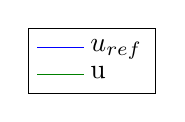
\begin{tikzpicture}

\begin{axis}[%
width=0.951\figurewidth,
height=\figureheight,
at={(0\figurewidth,0\figureheight)},
scale only axis,
every outer x axis line/.append style={black},
every x tick label/.append style={font=\color{black}},
every x tick/.append style={black},
xmin=0,
xmax=20,
xlabel={Time [s]},
every outer y axis line/.append style={black},
every y tick label/.append style={font=\color{black}},
every y tick/.append style={black},
ymin=-30,
ymax=40,
ylabel={Pitch [deg]},
axis background/.style={fill=white},
axis x line*=bottom,
axis y line*=left,
xmajorgrids,
ymajorgrids,
legend style={legend cell align=left, align=left, draw=black}
]
\addplot [color=blue]
  table[row sep=crcr]{%
0	0\\
0.25	0\\
0.5	0\\
0.75	0\\
1	0\\
1.25	0\\
1.5	0\\
1.75	0\\
2	0\\
2.25	0\\
2.5	0\\
2.75	0\\
3	0\\
3.25	0\\
3.5	0\\
3.75	0\\
4	0\\
4.25	0\\
4.5	0\\
4.75	0\\
5	30\\
5.25	30\\
5.5	30\\
5.75	30\\
6	30\\
6.25	30\\
6.5	30\\
6.75	30\\
7	30\\
7.25	30\\
7.5	18.611\\
7.75	7.8596\\
8	-0.96793\\
8.25	-8.0533\\
8.5	-13.58\\
8.75	-17.729\\
9	-20.676\\
9.25	-22.589\\
9.5	-23.627\\
9.75	-23.936\\
10	-23.651\\
10.25	-22.894\\
10.5	-21.772\\
10.75	-20.383\\
11	-18.808\\
11.25	-17.119\\
11.5	-15.376\\
11.75	-13.628\\
12	-11.915\\
12.25	-10.268\\
12.5	-8.712\\
12.75	-7.2631\\
13	-5.9332\\
13.25	-4.7289\\
13.5	-3.6526\\
13.75	-2.7035\\
14	-1.8782\\
14.25	-1.1711\\
14.5	-0.57496\\
14.75	-0.08161\\
15	0.31789\\
15.25	0.63282\\
15.5	0.87257\\
15.75	1.0464\\
16	1.1631\\
16.25	1.2313\\
16.5	1.2587\\
16.75	1.2528\\
17	1.2201\\
17.25	1.1665\\
17.5	1.0973\\
17.75	1.017\\
18	0.92959\\
18.25	0.83841\\
18.5	0.74621\\
18.75	0.65524\\
19	0.56729\\
19.25	0.48375\\
19.5	0.40561\\
19.75	0.33359\\
20	0.26809\\
20.25	0.20931\\
20.5	0.15727\\
20.75	0.11182\\
21	0.072691\\
21.25	0.03954\\
21.5	0.011946\\
21.75	-0.010551\\
22	-0.028434\\
22.25	-0.042198\\
22.5	-0.052331\\
22.75	-0.059309\\
23	-0.063585\\
23.25	-0.065585\\
23.5	-0.065703\\
23.75	-0.0643\\
24	-0.061699\\
24.25	-0.05819\\
24.5	-0.054025\\
24.75	-0.049426\\
25	-0.04458\\
25.25	-0.039645\\
25.5	-0.034753\\
25.75	-0.03001\\
26	-0.0255\\
26.25	-0.021289\\
26.5	-0.017424\\
26.75	-0.013939\\
27	-0.010856\\
27.25	-0.0081854\\
27.5	-0.0059278\\
27.75	-0.0040767\\
28	-0.0026171\\
28.25	-0.0015259\\
28.5	-0.00077034\\
28.75	-0.00030585\\
29	-7.3744e-05\\
29.25	1.4149e-13\\
29.5	1.4129e-13\\
29.75	0\\
30	0\\
30.25	0\\
30.5	0\\
30.75	0\\
31	0\\
31.25	0\\
31.5	0\\
31.75	0\\
32	0\\
32.25	0\\
32.5	0\\
32.75	0\\
33	0\\
33.25	0\\
33.5	0\\
33.75	0\\
34	0\\
34.25	0\\
34.5	0\\
34.75	0\\
35	0\\
};
\addlegendentry{$\text{u}_{\text{ref}}$}

\addplot [color=black!50!green]
  table[row sep=crcr]{%
0	0\\
0.1	3.8891\\
0.2	13.069\\
0.3	18.578\\
0.4	15.491\\
0.5	11.527\\
0.6	6.3965\\
0.7	5.2201\\
0.8	5.1716\\
0.9	4.7909\\
1	3.6643\\
1.1	3.5385\\
1.2	1.8505\\
1.3	2.158\\
1.4	1.4011\\
1.5	2.0717\\
1.6	-1.0543\\
1.7	0.28095\\
1.8	2.7854\\
1.9	1.6755\\
2	1.8848\\
2.1	0.90372\\
2.2	5.1923\\
2.3	4.1202\\
2.4	2.9455\\
2.5	2.8817\\
2.6	4.2333\\
2.7	4.4135\\
2.8	0.71441\\
2.9	2.3671\\
3	-2.2187\\
3.1	-1.0961\\
3.2	0.71498\\
3.3	2.8113\\
3.4	-2.7738\\
3.5	-0.25057\\
3.6	1.4153\\
3.7	-0.27016\\
3.8	-3.3794\\
3.9	0.039865\\
4	-2.6026\\
4.1	-0.40419\\
4.2	-2.0576\\
4.3	0.071863\\
4.4	-1.5723\\
4.5	-4.6775\\
4.6	-0.86006\\
4.7	-2.0833\\
4.8	2.5381\\
4.9	14.502\\
5	18.246\\
5.1	12.77\\
5.2	14.146\\
5.3	14.935\\
5.4	23.095\\
5.5	21.111\\
5.6	27.481\\
5.7	23.243\\
5.8	22.115\\
5.9	23.466\\
6	26.989\\
6.1	29.038\\
6.2	30.619\\
6.3	27.956\\
6.4	26.263\\
6.5	27.531\\
6.6	29.154\\
6.7	29.347\\
6.8	31.74\\
6.9	30.331\\
7	28.896\\
7.1	28.169\\
7.2	28.4\\
7.3	27.924\\
7.4	24.49\\
7.5	21.591\\
7.6	19.81\\
7.7	20.592\\
7.8	18.105\\
7.9	12.353\\
8	11.656\\
8.1	9.1221\\
8.2	7.5162\\
8.3	7.5917\\
8.4	7.1993\\
8.5	5.6563\\
8.6	3.8366\\
8.7	-2.8604\\
8.8	-0.48968\\
8.9	-2.8675\\
9	0.44916\\
9.1	-1.7121\\
9.2	-3.9483\\
9.3	-4.8704\\
9.4	-5.2418\\
9.5	-8.0966\\
9.6	-9.7672\\
9.7	-6.6236\\
9.8	-8.9435\\
9.9	-8.5913\\
10	-10.042\\
10.1	-9.5288\\
10.2	-13.579\\
10.3	-10.033\\
10.4	-13.09\\
10.5	-9.599\\
10.6	-14.182\\
10.7	-14.11\\
10.8	-12.94\\
10.9	-11.029\\
11	-8.7047\\
11.1	-9.5062\\
11.2	-10.015\\
11.3	-12.398\\
11.4	-9.0357\\
11.5	-6.3265\\
11.6	-7.1014\\
11.7	-7.9861\\
11.8	-5.541\\
11.9	-4.9852\\
12	-3.4008\\
12.1	-4.5882\\
12.2	-5.8007\\
12.3	-4.7406\\
12.4	0.94885\\
12.5	-3.3568\\
12.6	-1.2845\\
12.7	-3.7315\\
12.8	-2.7047\\
12.9	-3.3854\\
13	-0.39743\\
13.1	-0.18236\\
13.2	-1.3033\\
13.3	-0.77305\\
13.4	-1.9294\\
13.5	1.0899\\
13.6	2.5925\\
13.7	-2.3257\\
13.8	-0.55549\\
13.9	0.84302\\
14	-1.5813\\
14.1	3.1234\\
14.2	3.2572\\
14.3	3.6754\\
14.4	-0.56035\\
14.5	0.60382\\
14.6	1.2002\\
14.7	1.5691\\
14.8	-0.18381\\
14.9	0.88166\\
15	3.5335\\
15.1	4.3344\\
15.2	-0.39473\\
15.3	1.2982\\
15.4	2.1377\\
15.5	-0.13956\\
15.6	2.4717\\
15.7	3.5174\\
15.8	1.3382\\
15.9	0.64484\\
16	-0.28448\\
16.1	2.7124\\
16.2	6.0537\\
16.3	6.1561\\
16.4	-0.157\\
16.5	1.6918\\
16.6	5.1149\\
16.7	2.798\\
16.8	1.3679\\
16.9	4.5548\\
17	1.2994\\
17.1	1.6912\\
17.2	-0.50307\\
17.3	0.042934\\
17.4	1.7973\\
17.5	-0.82232\\
17.6	2.2139\\
17.7	0.8421\\
17.8	2.3656\\
17.9	3.43\\
18	2.9348\\
18.1	3.0866\\
18.2	5.0725\\
18.3	2.7491\\
18.4	4.4592\\
18.5	0.18739\\
18.6	4.3278\\
18.7	3.111\\
18.8	3.4936\\
18.9	-0.82925\\
19	2.5902\\
19.1	1.5257\\
19.2	0.96343\\
19.3	4.6405\\
19.4	1.5688\\
19.5	2.5212\\
19.6	2.3218\\
19.7	0.57722\\
19.8	1.0625\\
19.9	2.2768\\
20	0.44441\\
20.1	0.94889\\
20.2	-0.91107\\
20.3	-1.7993\\
20.4	2.3012\\
};
\addlegendentry{u}

\end{axis}
\end{tikzpicture}%
        \caption{U, \(p_{ref}\) and Optimal U, Q = diag[50,0,0,0]} 
\label{fig:ex3_u} 
\end{figure} 



\end{document}